\begin{frame}
	\titlepage 
\end{frame}

\begin{frame}{Institut des sciences de la Terre, Grenoble}
	\begin{itemize}
		\item 280 personnes, dont 108 chercheurs et 80 doctorants (2016)
		\item Géochimie (géologie, minéralogie)
		\item Géophysique (mécanique, ondes, tectonique, cycle sismique, magnétisme)
		\item Risque et environnement
	\end{itemize}
	
		
	\vfill
	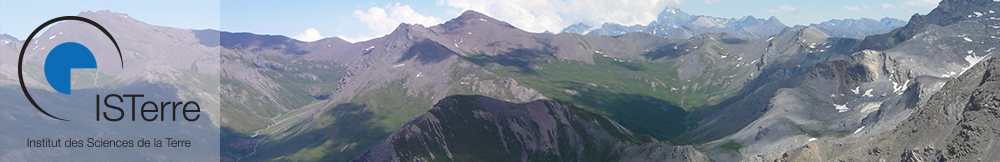
\includegraphics[width=\textwidth]{img/bandeau_isterre.jpg}
\end{frame}

\begin{frame}{Imagerie US vs localisation de sources}
	\begin{itemize}
		\item<1-> Localisation de sources acoustiques
		\begin{figure}
			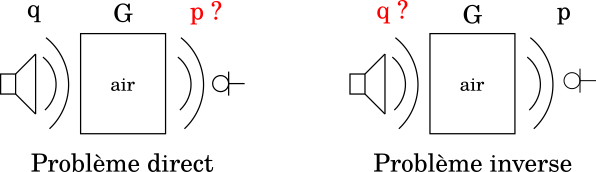
\includegraphics[width = 6cm]{./img/pd_dir_inv/ac.png}
		\end{figure}~\\
		\item<2-> Imagerie par ultrasons
		\begin{figure}
			
\includegraphics[width = 6cm]{./img/pd_dir_inv/us.png}
		\end{figure}
	\end{itemize}
	
\end{frame}

\begin{frame}{Projet Seiscope}
	\begin{columns}
		\column{0.6\textwidth}
		\centering
		\begin{itemize}
			\item $\approx$ 20 personnes à ISTerre
			\item Sponsors : industrie du gaz et pétrole
		\end{itemize}
		\column{0.45\textwidth}
		\centering
		\begin{figure}
			\vspace{-1cm}
			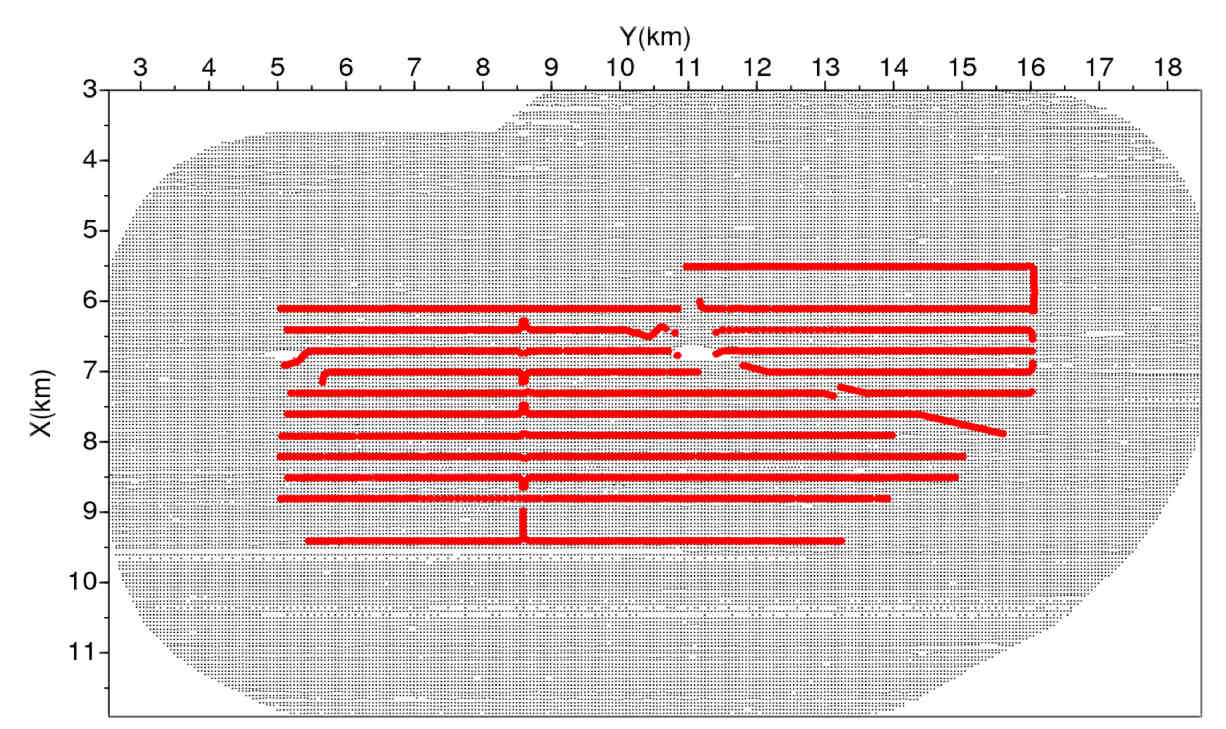
\includegraphics[width=0.9\textwidth]{img/dispo_valhall.jpg}\\
			{ \centering \scriptsize{Acquisition à Valhall, \itshape{ Sirgue et al. 2009}}\\
			120 km de câbles, 2414 hydrophones\\[-0.1cm]
			 50000 excitations par canon à air (45 km$^2$)}
		\end{figure}
	\end{columns}
	
	\begin{figure}
		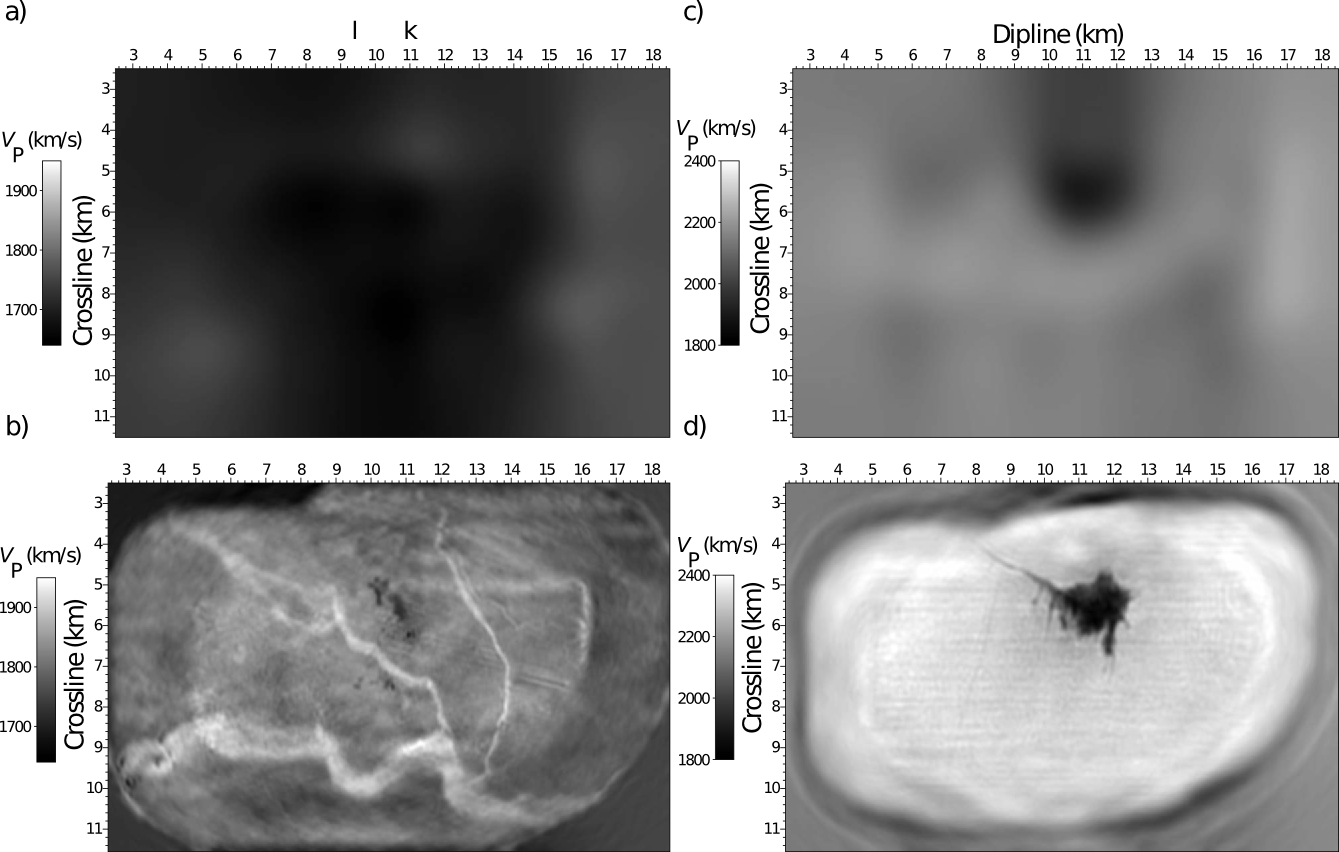
\includegraphics[width=0.6\textwidth]{img/geophy.png}\\
		\centering{\scriptsize Profondeur : 150 m~~~~~~Profondeur : 1050 m\\
		En haut : tomographie des temps en réflexion\\[-0.1cm]
		En bas : Inversion de forme d'ondes}
	\end{figure}
\end{frame}


\section{Contexte}

\subsection*{}
\begin{frame}{\insertsectionhead}
\vspace{-0.2cm}
		\begin{columns}
			\column{0.5\textwidth}
			\centering
			\begin{figure}
				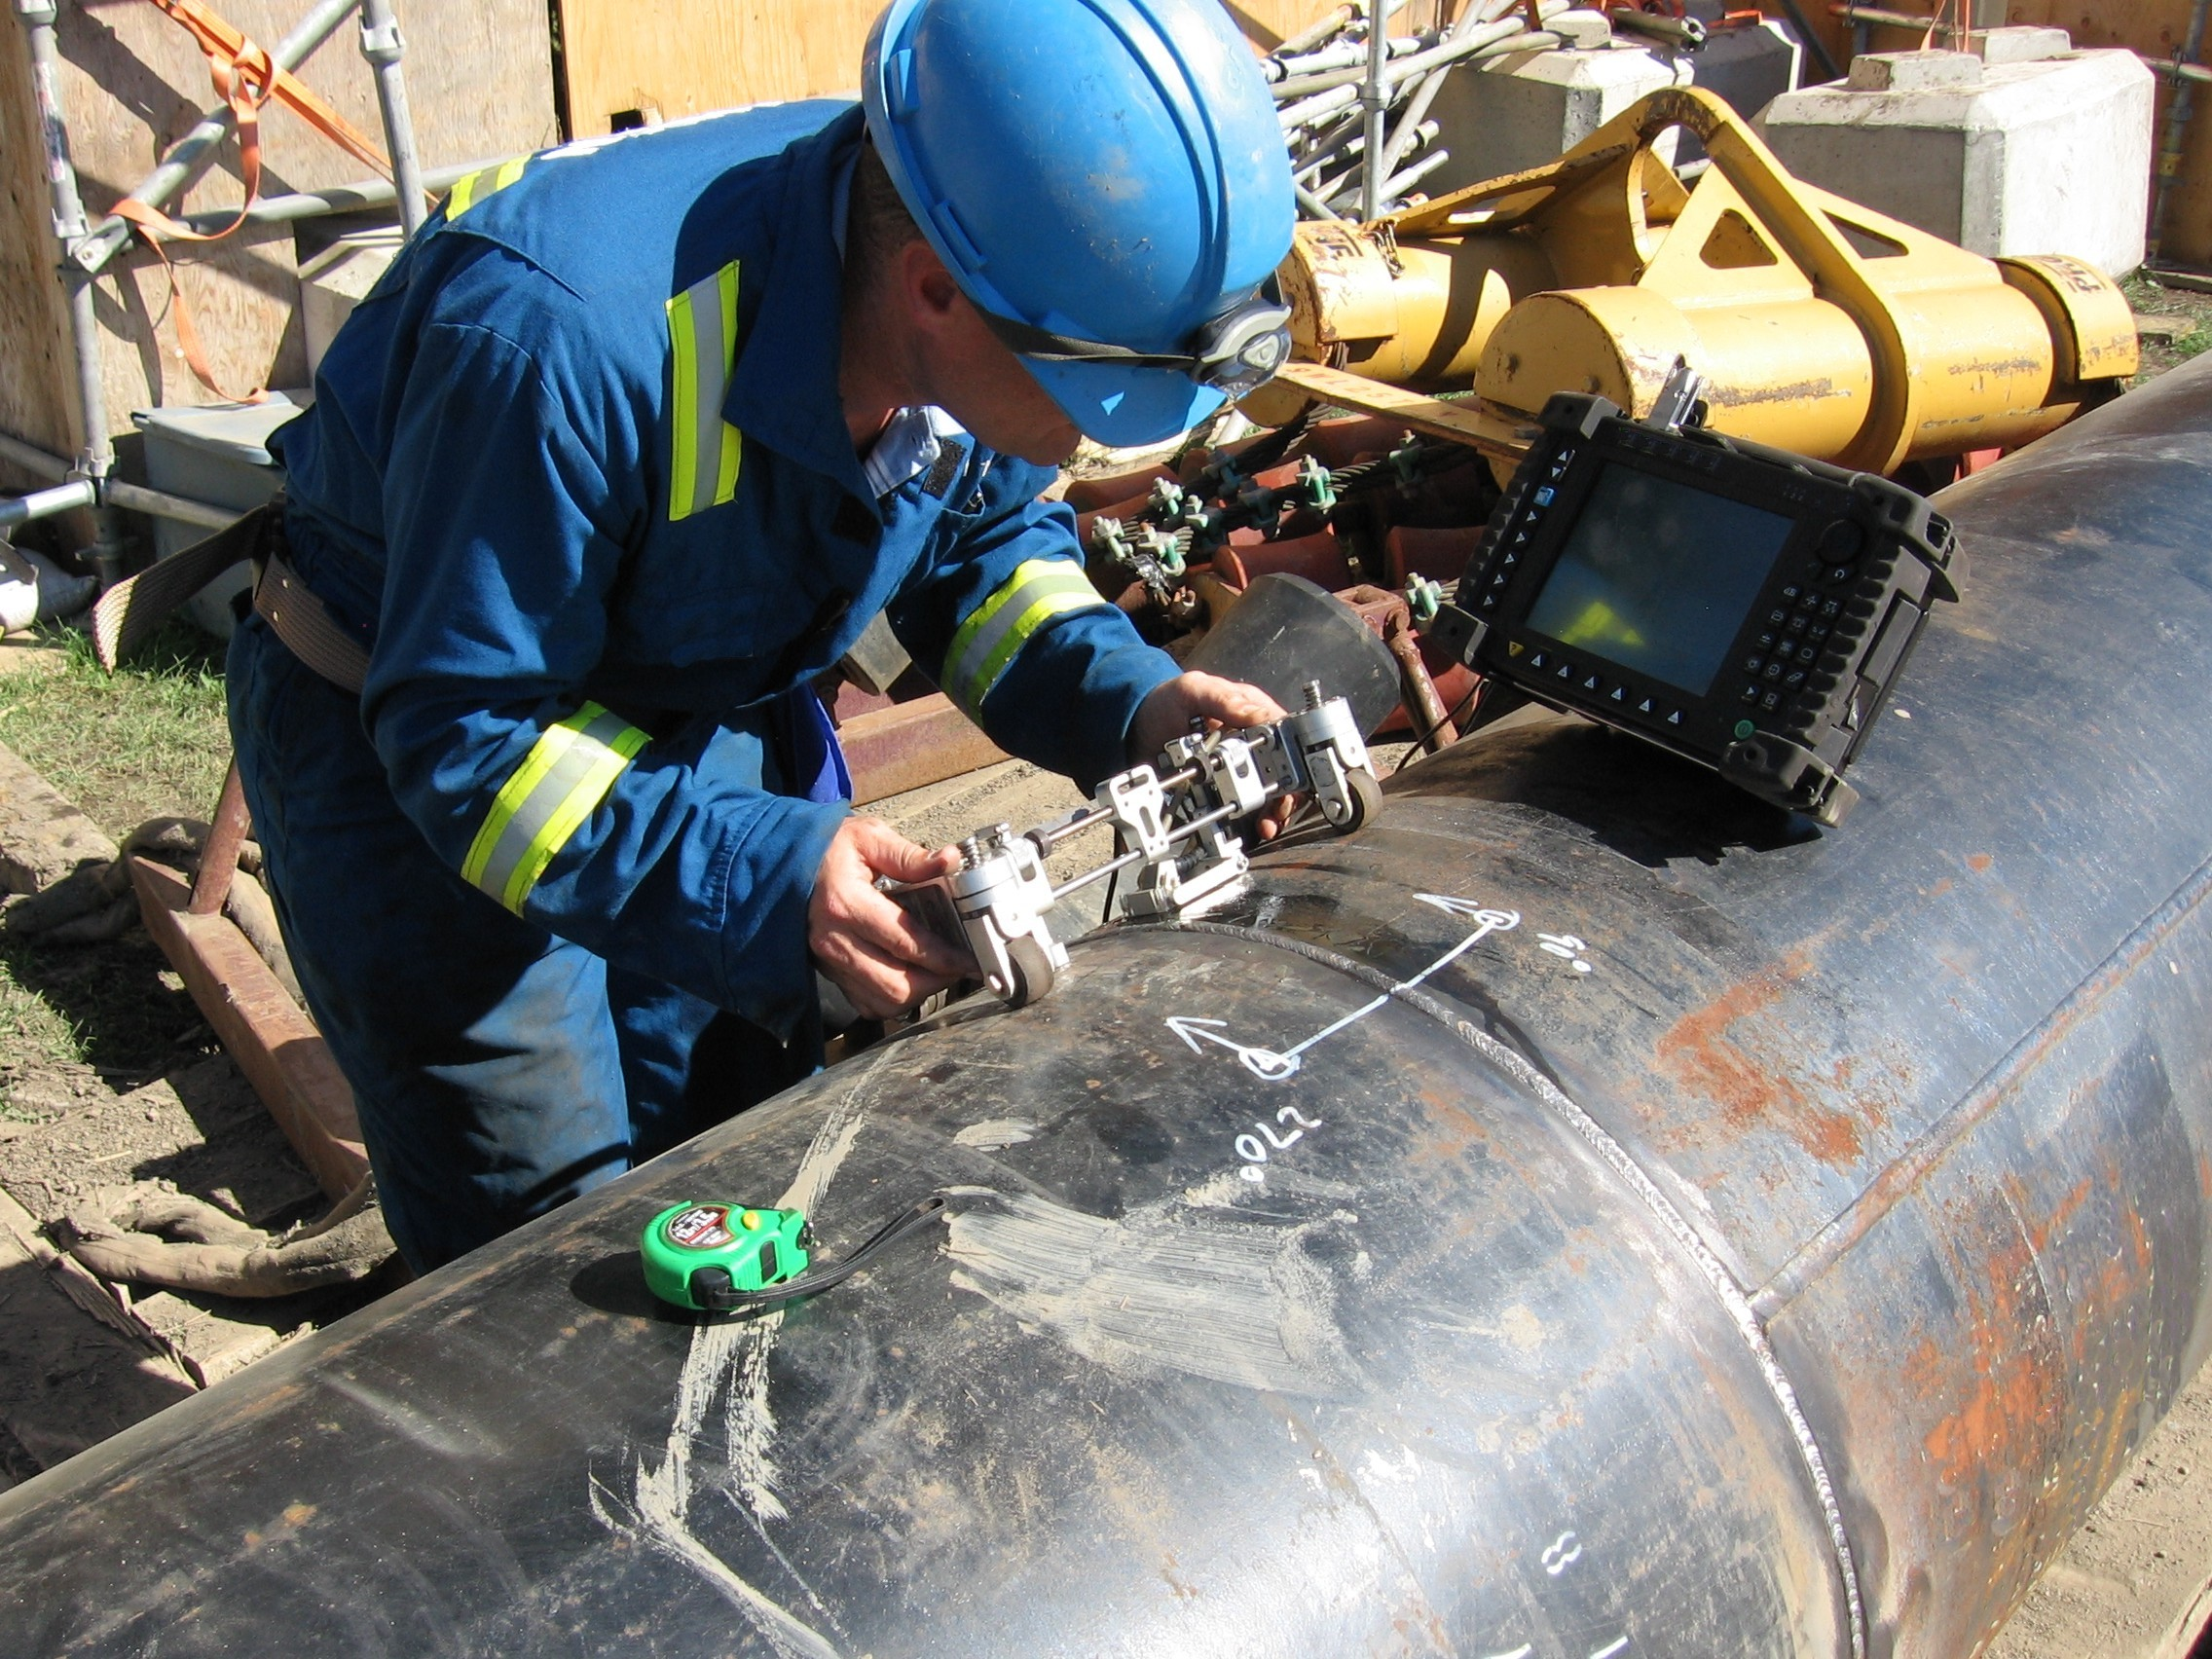
\includegraphics[height=3cm]{./img/us_test.jpg}\\
				{\tiny{\raggedright \itshape Image Davidmack}\\ \centering \scriptsize{Contrôle sur pipeline}}
			\end{figure}		
			\column{0.5\textwidth}
			\begin{figure}
				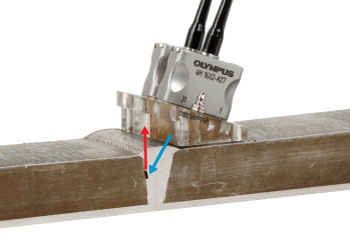
\includegraphics[height=3cm]{./img/olympus.jpg}\\
				 {\tiny{\itshape Image Olympus}\\ \centering			\scriptsize{Exemple de test en réflexion}}
			\end{figure}
		\end{columns}	
		\vspace{0.4cm}	

	%\begin{columns}
			%\column{.5\textwidth}
			Contrôle et évaluation de soudures :\\
			\begin{itemize}
				\item de centrales nucléaires (système de refroidissement)
				\item de pipelines 
			\end{itemize}
			%\column{.05\textwidth}
			%\ding{222}
			%\column{.45\textwidth}
			%\centering
			\vspace{-0.4cm}
			\begin{columns}
			\column{0.7\textwidth}
			\centering
 			\indent \ding{222} porosité, fissure, manque de fusion, corrosion, corps étrangers,\ldots
 			\column{0.3\textwidth}
 			\centering
 			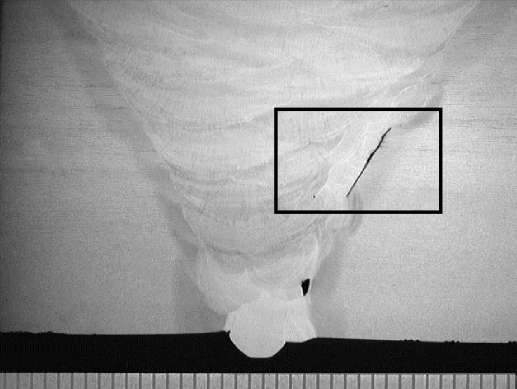
\includegraphics[width=0.95\textwidth]{./img/defaut_soudure.png}\\
 			{\itshape \tiny Image extraite de Consonni et al., \\[-0.2cm]Insight, 2011}
 			\end{columns}
	%\end{columns}
\end{frame}

\begin{frame}{Spécificité de l'imagerie de soudure}
	\begin{itemize}
		\item <1-> 2 surfaces libres : réflexions multiples $\leftrightarrow$ problème mal posé
		\item <2-> Acquisition de surface : limitation de la résolution 
		\item <3-> Anisotropie $\rightarrow$ inversion multiparamétrique \\\hspace{2.3cm}($C_{ij}\times$6 : soudure + défaut)
		%\item <4-> defects $\rightarrow$ multi-scale inversion ($C_{ij}^{d}\times$6)
	\end{itemize}
	\vfill
	\begin{figure}[!h]
		\centering
		\includegraphics<1-1>[scale=1]{img/soud1.pdf}
		\includegraphics<2-2>[scale=1]{img/soud2.pdf}
		%\includegraphics<3-3>[scale=1]{img/soud3.pdf}
		\includegraphics<3-3>[scale=1]{img/soud4_bis.pdf}
	\end{figure}

\end{frame}


\subsection*{}
\begin{frame}{\insertsectionhead}
\begin{small}
\vspace{-0.5cm}
\hspace{1cm}
\onslide<2->{
\begin{picture}(0,0)(0,0)\put(50,5){
		\textcolor{red}{Forte anisotropie imprévisible}
}\end{picture}
}
	\begin{columns}[c]
			\column{.5\textwidth}<1->
			\centering
			\begin{figure}
				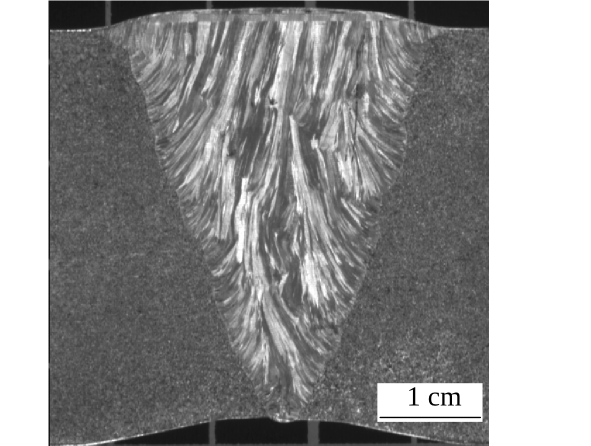
\includegraphics[height=2.7cm]{./img/soudure1.png}\\
				{\tiny{ \itshape Image extraite de Chassignole, 2010} \\ \centering \scriptsize Macrographie d'une soudure austénitique  }
			\end{figure}
			\column{.001\textwidth}<2->
			\hspace{-2.8cm}
			\vspace{2.5cm}
			\begin{tikzpicture}
					\draw[<-, thick,shorten <=2pt,shorten >=2pt,red] (-1.5,3)--(0.0,4.6);
			\end{tikzpicture}
			\column{.9\textwidth}<2->
			%\vfill
			\hspace{-1cm}
			$\hookrightarrow$ déviation et division du faisceau ultrasonore\\[0.2cm]
			\hspace{-0.5cm}
			\hspace{1cm}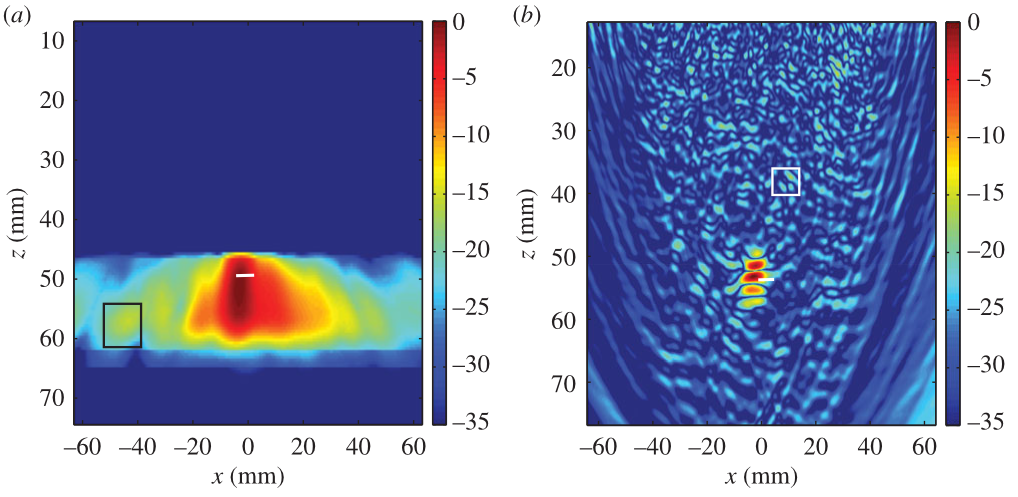
\includegraphics[height=2.5cm]{img/tfm_dort.png}\\
			{\tiny{ \itshape  \hspace{1.7cm} Cunningham et al., Proc. R. Soc., 2016} \\[0.2cm] \hspace{1cm} \scriptsize Méthodes DORT (gauche) et FTP (droite)\\[-0.1cm] \hspace{1.5cm}sur modèle EF de soudure anisotrope }
				
	\end{columns}
	%\vspace{0.3cm}
	\begin{columns}[c]
			\column{.5\textwidth}<1->
			%\begin{block}{}
				\begin{itemize}
					\item[$\bullet$] méthodes par sommation cohérente des signaux (ex : FTP)
					\item[$\bullet$] Décomposition des matrices de covariance (ex : DORT)
				\end{itemize}
			%\end{block}
			\column{.05\textwidth}<2->
			\ding{222}
			\column{.5\textwidth}<2->
				\begin{itemize}
					\item[\ding{55}] requièrent une connaissance\\ \emph{a priori} de la vitesse\\
					\item[\ding{55}] sujettes aux artefacts
				\end{itemize}
	\end{columns}
	\vspace{0.1cm}
	\begin{columns}[c]
		\column{.5\textwidth}<3->
			\begin{itemize}
				\item[$\bullet$] Résolution d'un problème d'optimisation
			\end{itemize}
		\column{.05\textwidth}<3->
			\ding{222}
		\column{.5\textwidth}<3->
			\begin{itemize}
			%\item optimisation topologique :\\\hspace{-0.5cm}\small{\emph{Dominguez et al.}, \emph{Rodriguez et al.}}\\[0.1cm]
			\item[\ding{51}] {reconstruction d'un ensemble de paramètres : FWI}
		\end{itemize}		
	\end{columns}
\end{small}
\end{frame} 


\section{La FWI}
\subsection*{}
\begin{frame}{Full Waveform Inversion}
	\begin{columns}
		\column{0.6\textwidth}<1->
		\begin{itemize}
			\item<2-> Fonction de coût : $C(\bm{m})=\frac{1}{2}||\bm{d}_{obs}-\bm{d}_{cal}(\bm{m})||^{2}$\\[0.3cm]
			\item<3-> Optimisation locale : modèle optimal quand $C'(\bm{m} + \bm{\Delta m})=0$\\[0.3cm]
			%\item[$\hookrightarrow$]  ~\\[0.5cm]
			\item<4-4> Perturbation du modèle : $\bm{\Delta m}=-(C'')^{-1}$\fcolorbox{white!0}{white!0}{$C'$}\\[0.3cm]
			$C''$ : approx. à partir de $C'$ (L-BFGS)\\
			$C'$ : ?
		\end{itemize}

		
		\column{0.5\textwidth}<1->
		\begin{figure}
			\centering
			\hspace{-0.3cm}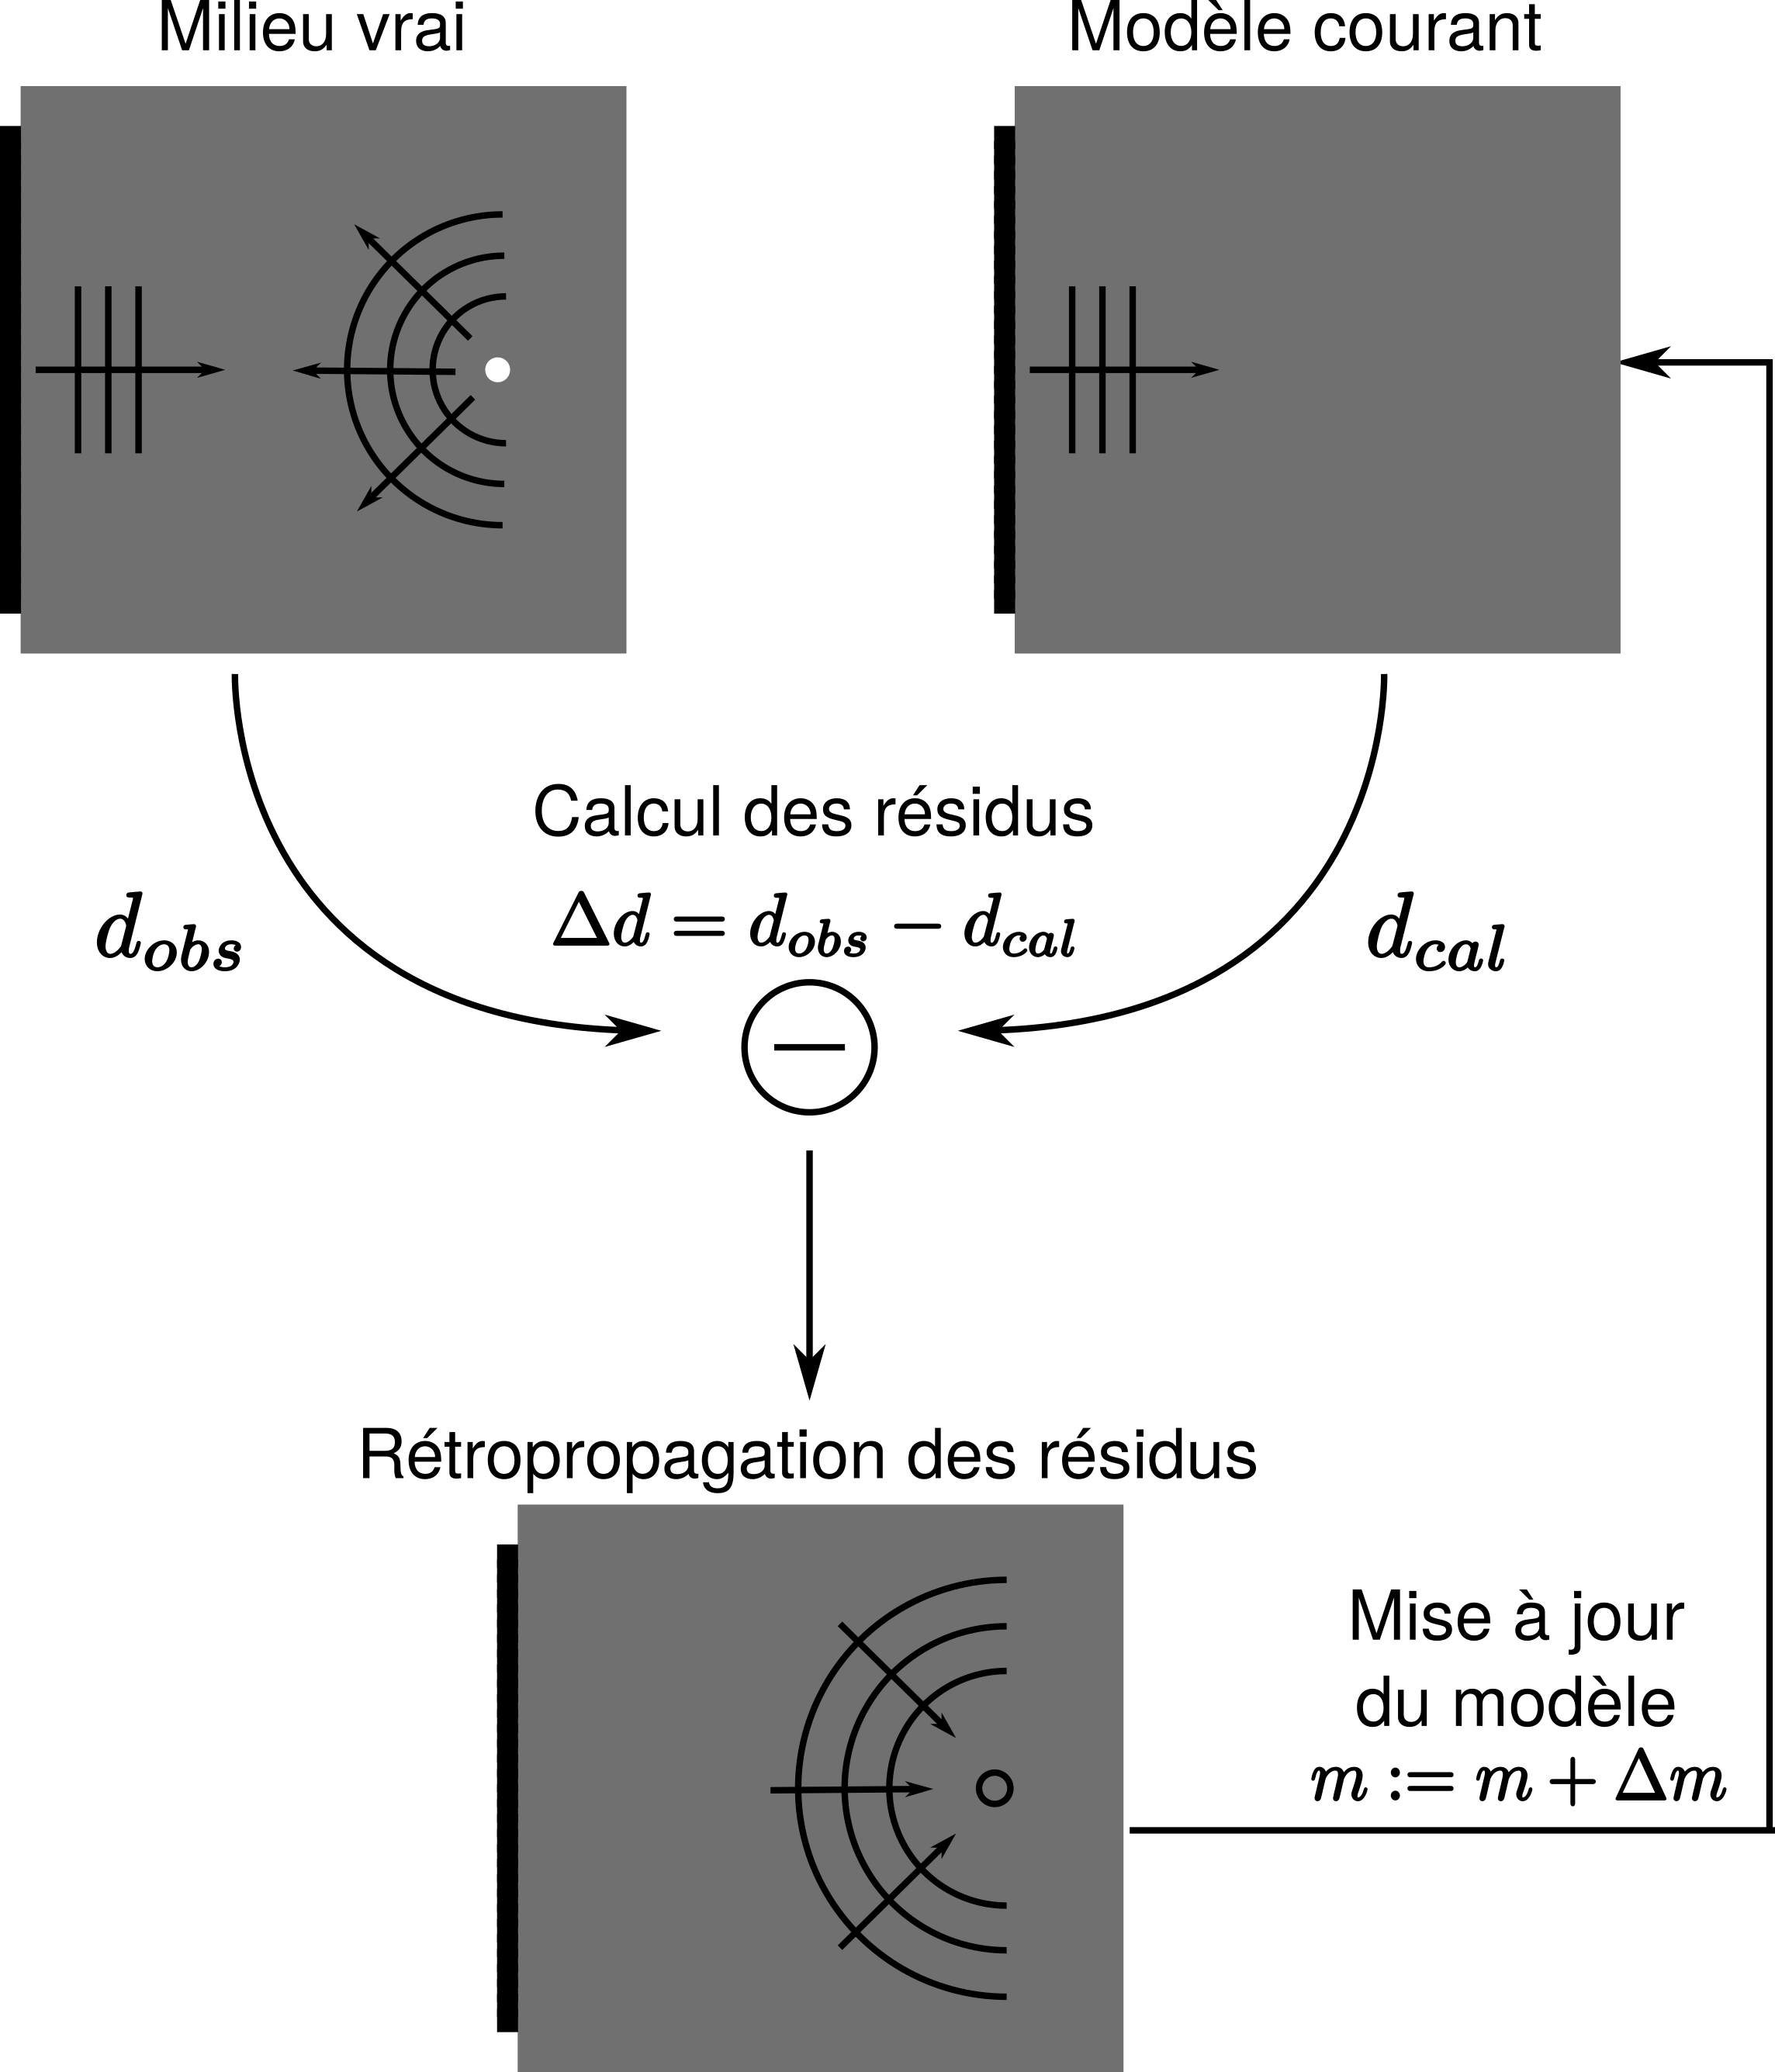
\includegraphics[width=\textwidth]{img/schema_fwi2.png}
		\end{figure}
	\end{columns}
	
\end{frame}

\begin{frame}{Calcul du gradient}
	\begin{itemize}
%		\item<1-> Problème direct...
%		\begin{equation*}
%			\bm{A}(\bm{m},\bm{x},t)\bm{d}_{cal}(\bm{m},\bm{x},t)=\bm{s}(\bm{x},t)
%		\end{equation*}
%	
%		\item<2->...dérivé par rapport à $\bm{m}$ : 
%		\begin{equation*}
%			\bm{A} \frac{\partial \bm{{d}}_{cal}(\bm{m})}{\partial m_{i}} + \frac{\partial \bm{A}}{\partial m_{i}}\bm{{d}}_{cal}(\bm{m}) = \bm{0} 
%		\end{equation*}
		\item Fonction de coût : $C(\bm{m})=\frac{1}{2}||\bm{d}_{obs}-\bm{d}_{cal}(\bm{m})||^{2}$\\
		\item<2->Expression du gradient	
		\begin{equation*}
			\frac{\partial C (\bm{m})}{\partial m_{i}} = -\tr{\left( \frac{\partial \bm{d}_{cal}(\bm{m}) }{\partial m_{i}} \right)} ( \bm{d}_{obs} - \bm{d}_{cal}(\bm{m})) 			
		\end{equation*}
		\onslide<3->{
		\begin{equation*}
			C'= \tr{{\bm{d}}_{cal}} \tr{\left( \frac{\partial\bm{A}}{\partial m_{i}} \right)} \textcolor{DeepSkyBlue4}{\underbrace{\textcolor{black}{\bm{A}^{-1} ({\bm{d}}_{obs} - {\bm{d}}_{cal})}}_{\text{résidus rétropopagés}}}
		\end{equation*}
		}
	\end{itemize}
	
	\onslide<4->{\textbf{Le gradient découle du calcul de 2 problèmes directs :}
	\begin{equation*}
		\bm{A}(\bm{m})\bm{{d}}_{cal}(\bm{m})=\bm{s} ~~~~~~~\text{et}~~~~~~~\bm{A}(\bm{m})\bm{\lambda} (\bm{m})=( \bm{{d}}_{obs} - \bm{{d}}_{cal}(\bm{m})),
	\end{equation*}
	}
	
\end{frame}


\section{Résolution de la FWI}

\subsection*{}
\begin{frame}{\insertsectionhead}
	\only<1-3>{
		\begin{equation*}
			C'= \textcolor{DeepSkyBlue4}{\underbrace{\textcolor{black}{\tr{{\bm{d}}_{cal}}}}_{\substack{\text{champ incident}}}}
			  \text{\fcolorbox{white!0}{white!0}{$\tr{\left( \frac{\partial\bm{A}}{\partial m_{i}} \right)}$ }} 
			 \textcolor{DeepSkyBlue4}{\underbrace{\textcolor{black}{\bm{\lambda}}}_{\substack{\text{résidus rétropopagés}}}}
		\end{equation*}
	}
	\only<4->{
		\vspace{-0.06cm}\begin{equation*}
			C'= \textcolor{DeepSkyBlue4}{\underbrace{\textcolor{black}{\tr{{\bm{d}}_{cal}}}}_{\substack{\text{champ incident}}}}
			 \text{\fcolorbox{DeepSkyBlue4}{white!0}{$\tr{\left( \frac{\partial\bm{A}}{\partial m_{i}} \right)}$ }}
			 \textcolor{DeepSkyBlue4}{\underbrace{\textcolor{black}{\bm{\lambda}}}_{\substack{\text{résidus rétropopagés}}}}
		\end{equation*}		
%	\begin{picture}(0,0)(0,0)\put(155,-105){
%		\begin{tikzpicture}	
%					\node (A) at (6,0) {};
%					\node (ray) at ($(A)+(0,-4)$) {};
%					\draw[->, thick,shorten <=2pt,shorten >=2pt,DeepSkyBlue4] (A) -- (ray);		
%		\end{tikzpicture}
%	}\end{picture}
	}
	\begin{equation*}
		~~~~~~~~\sim~ \Re\left( e^{j k_{0} \bm{s.x}} \right)~~~~~~~~~\sim~ \Re\left( e^{j k_{0} \bm{r.x}} \right)
	\end{equation*}
		
	\onslide<2->{
		\begin{itemize}
			\item Résolution du gradient :\vspace{-0.34cm}
			\begin{align}
				k=k_0|\bm{s}+\bm{r}|=&\frac{\omega}{c}2\cos\left( \frac{\theta}{2} \right)~~~~~~~~\\
				\hookrightarrow \text{~ maximale ($\lambda$/2) en HF et pour}~&\theta=0 \nonumber
			\end{align}	\vspace{-1cm}		
	}
		\only<1-3>{
			\begin{columns}
				\column{0.4\textwidth}<1-3>
				\begin{figure}
					\centering
					\vfill
					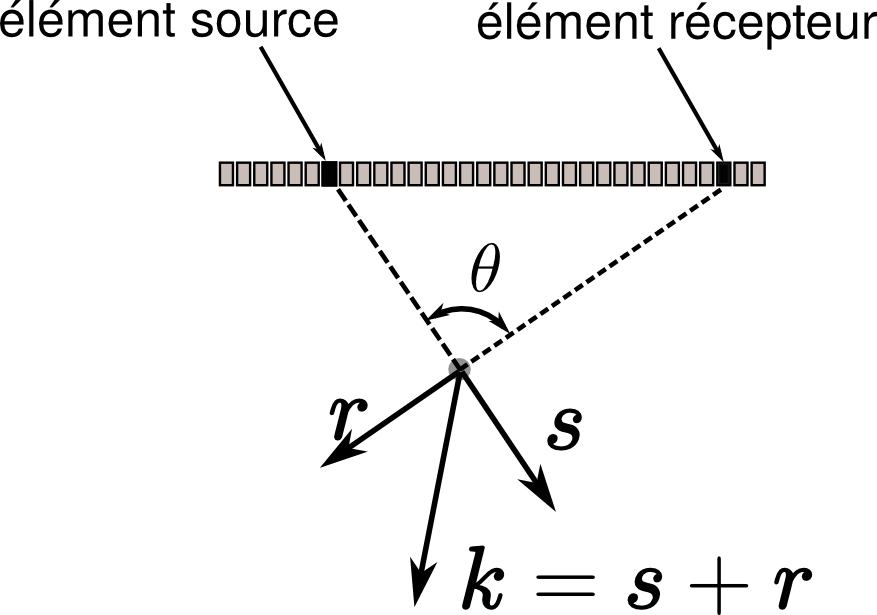
\includegraphics[height=2.5cm]{img/reso.png}	
				\end{figure}
				\column{0.55\textwidth}<3-3>
				\begin{figure}
					\centering
					\vspace{0.4cm} 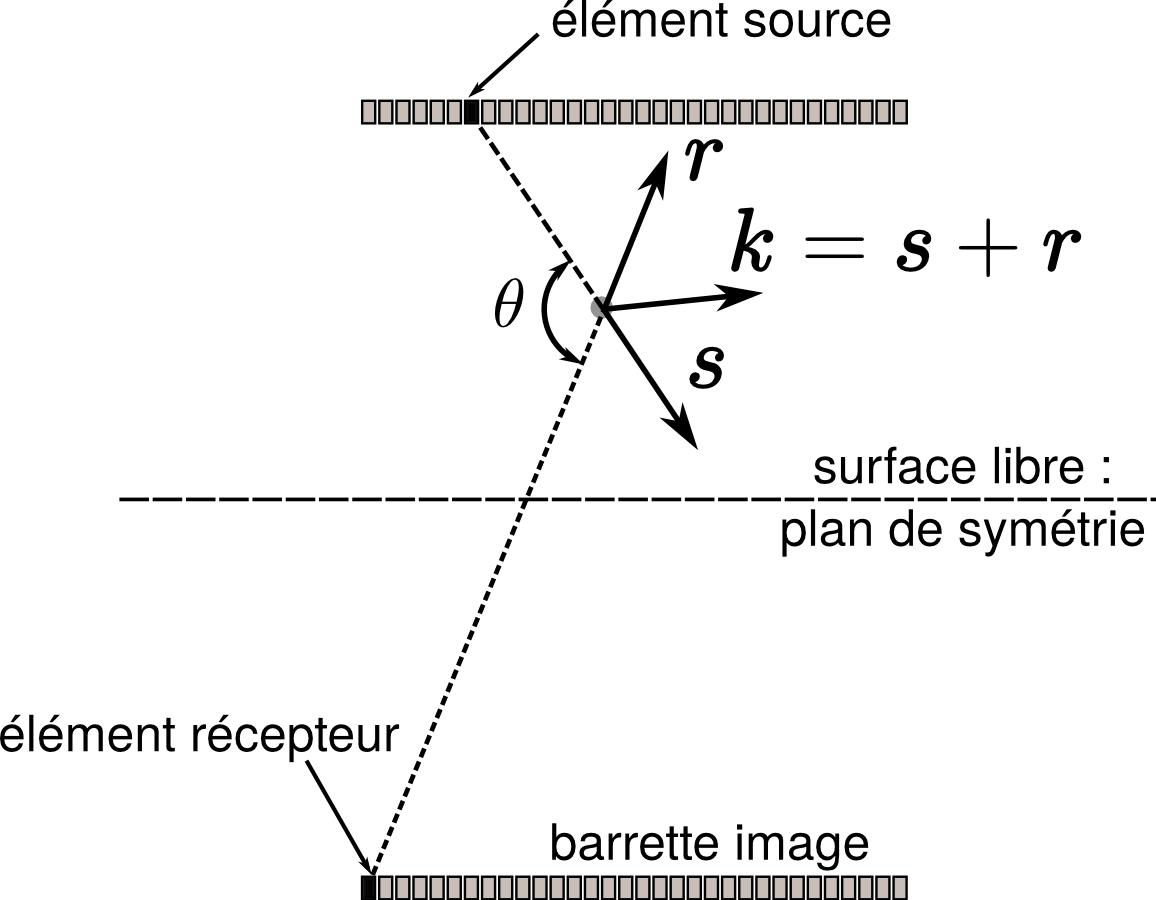
\includegraphics[height=3.7cm]{img/reso_surf_libre.png}
				\end{figure}		
			\end{columns}
		}	

	\only<4->{		
		\vspace{0.7cm}\item Rayonnement des paramètres :\\[0.2cm] 
		\begin{figure}
			\hspace{-1cm}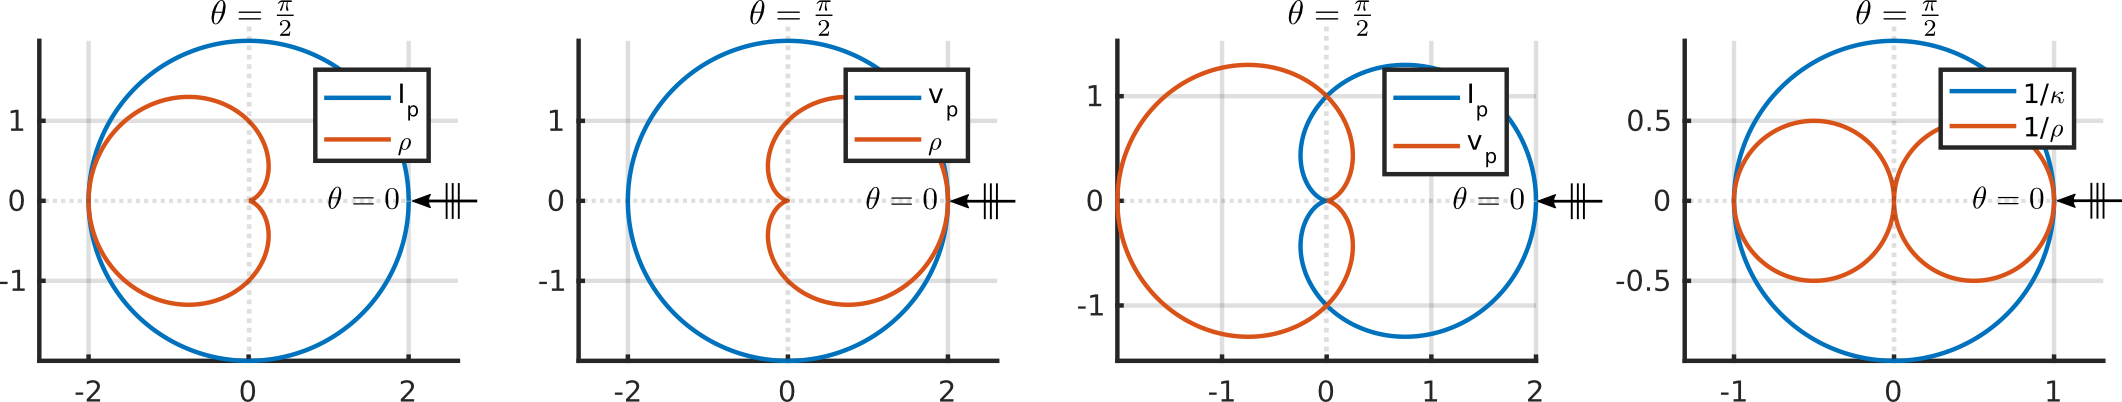
\includegraphics[height=2cm]{img/rayonnement.png}
		\end{figure}		
	}

	\end{itemize}
	\vspace{1cm}
\end{frame}


\begin{frame}{Résolution de la FWI}
	\begin{figure}
		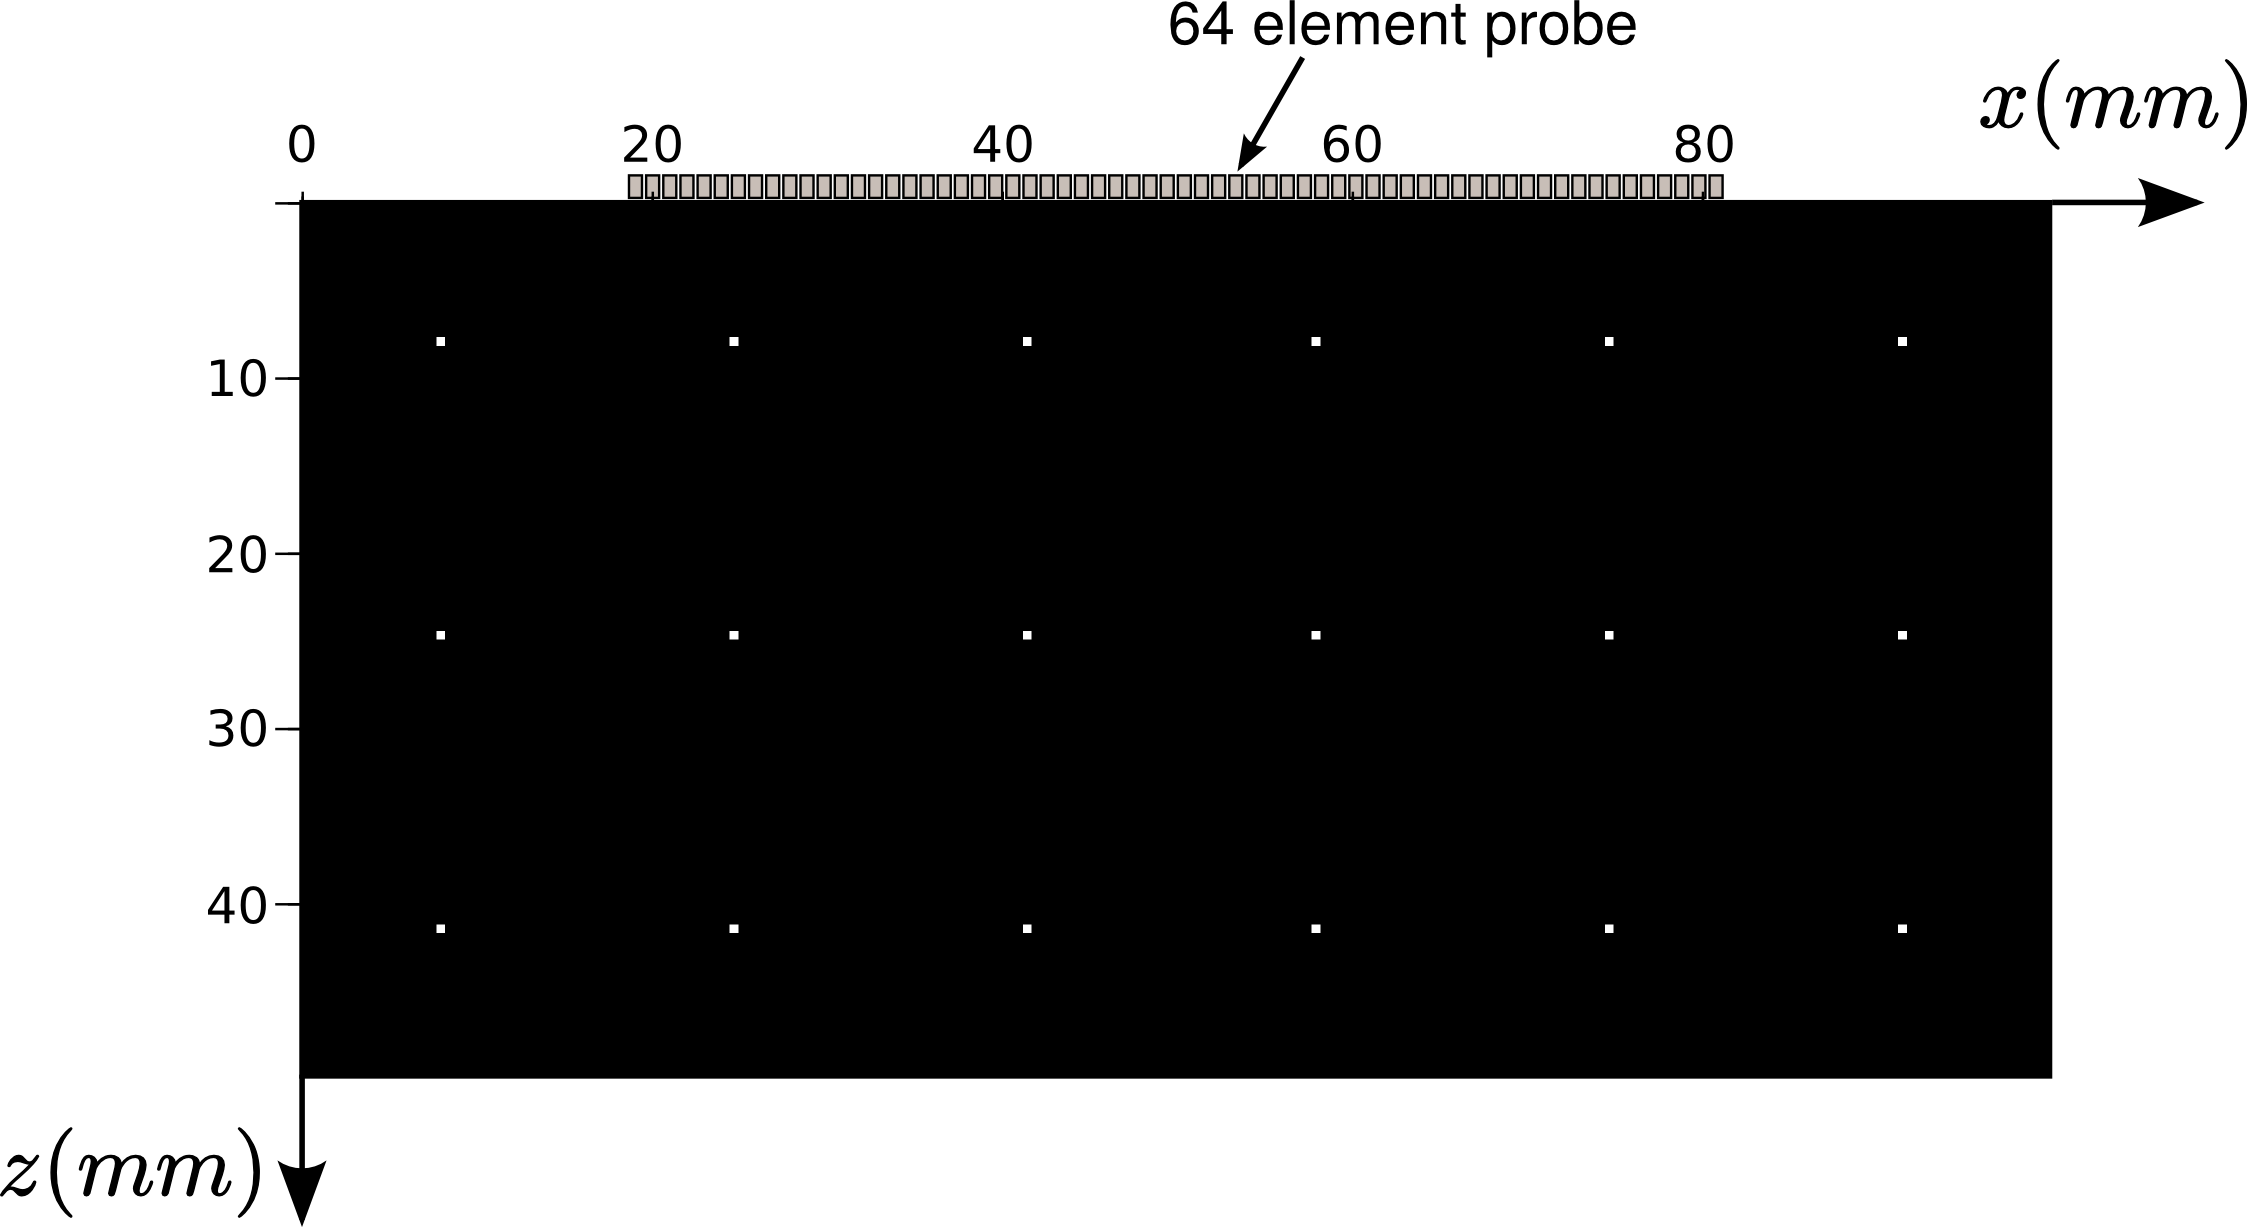
\includegraphics[height=2.5cm]{img/vp_scat.png}\\
		\vspace{-0.3cm} \small{Modèle de vitesse}
	\end{figure}
	\vspace{-0.6cm} 
	\begin{columns}
		\column{0.5\textwidth}
		\begin{figure}
			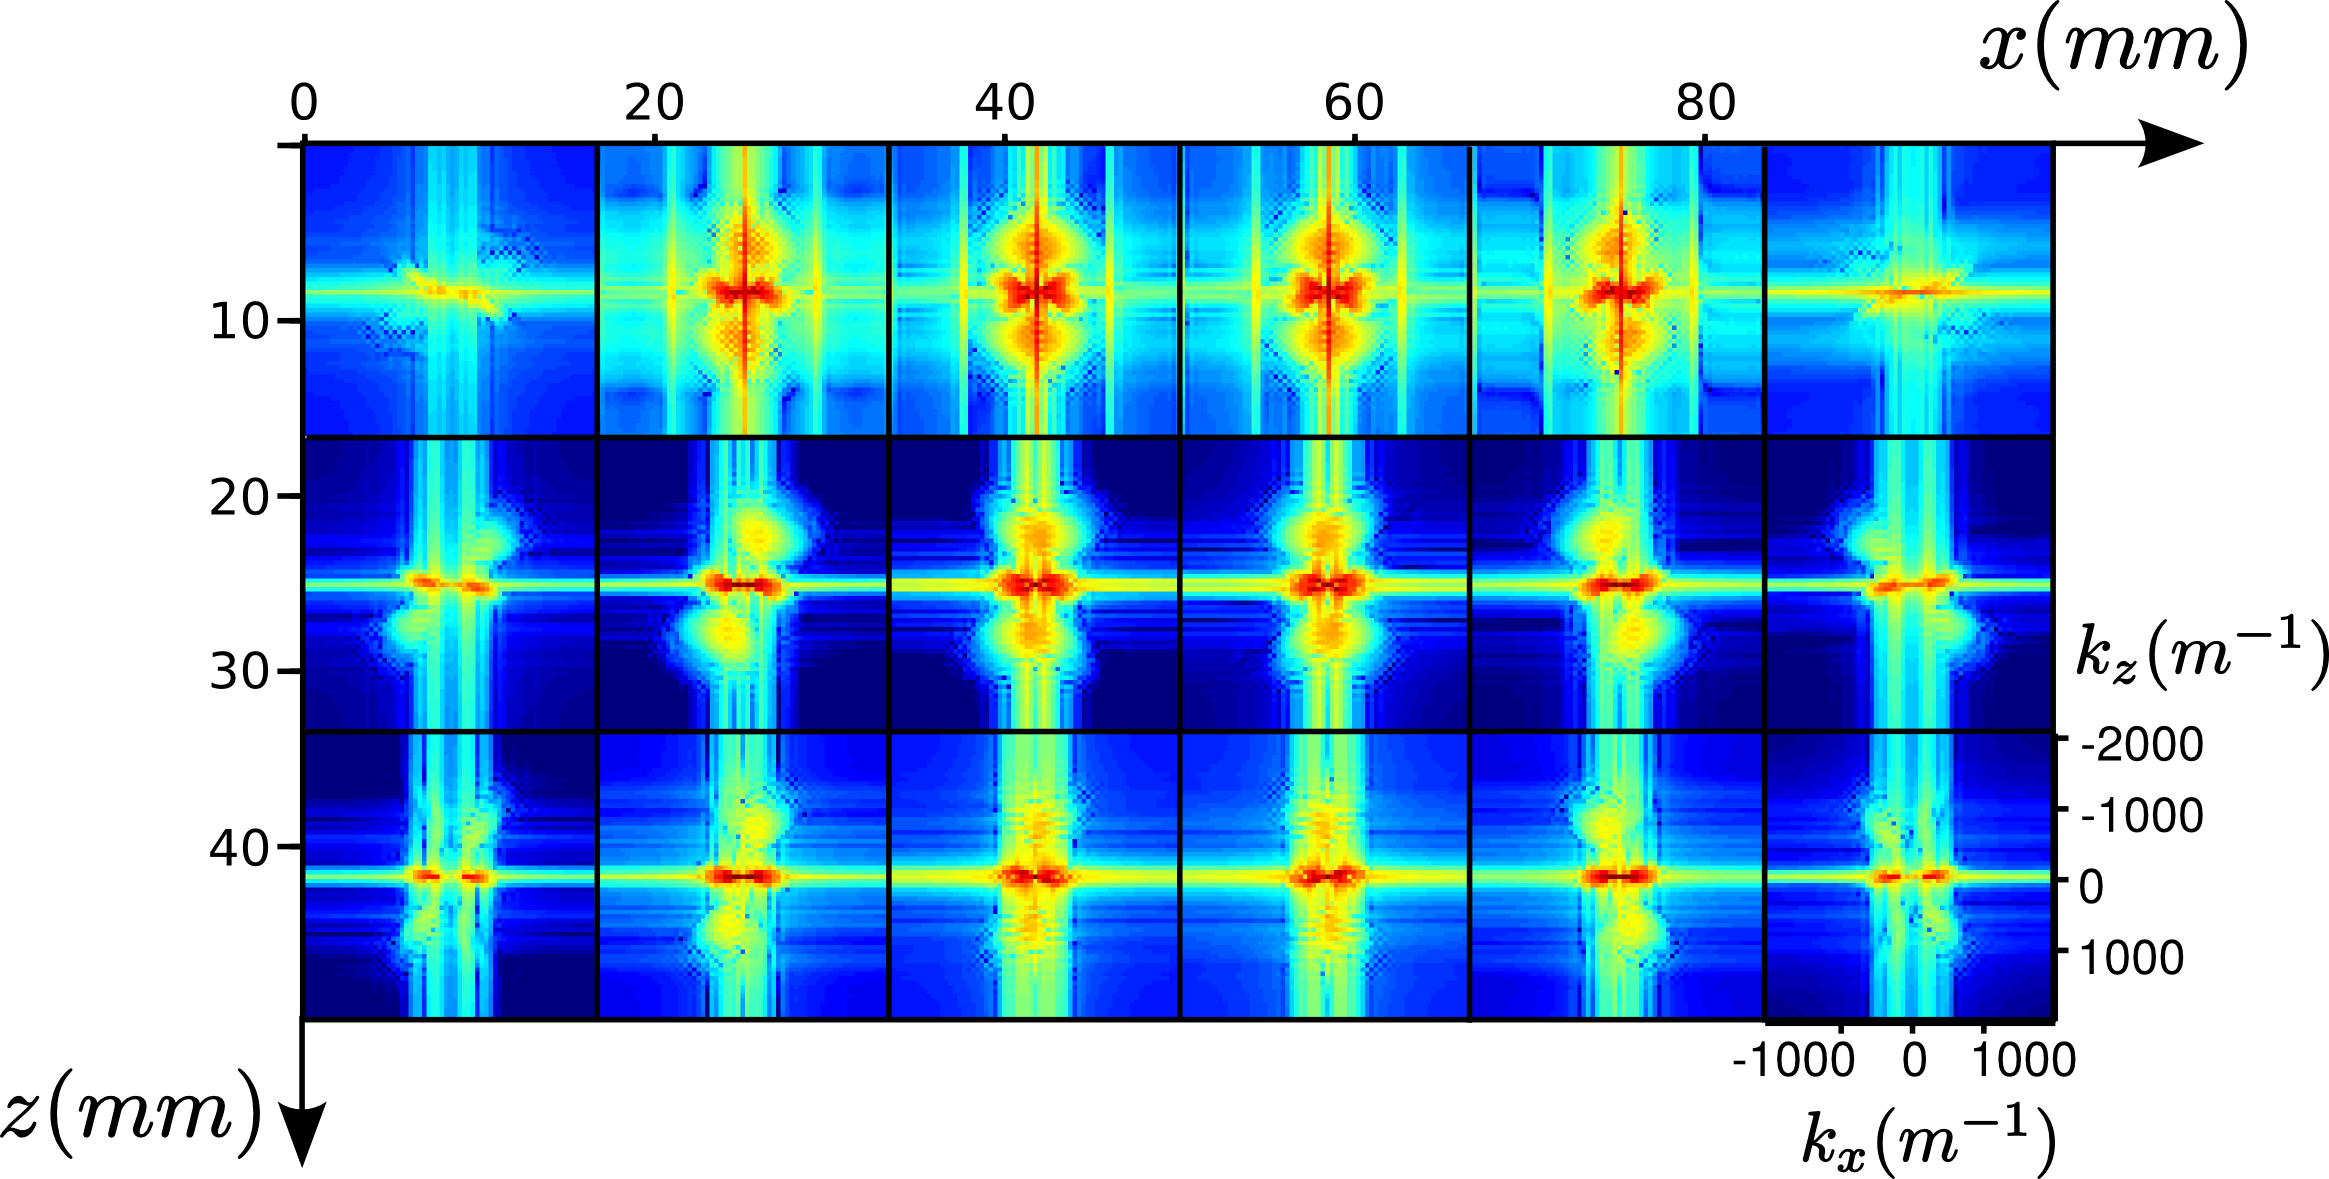
\includegraphics[height=3cm]{img/1400pt.png}\\
			\small{Pour 1 réflexion}\\[0.3cm]
			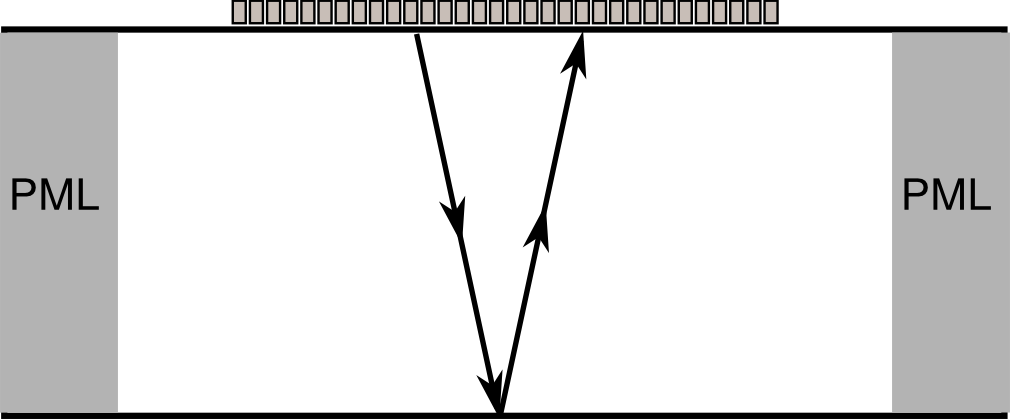
\includegraphics[height=1cm]{img/1ref.png}
		\end{figure}
		\column{0.5\textwidth}
		\begin{figure}
			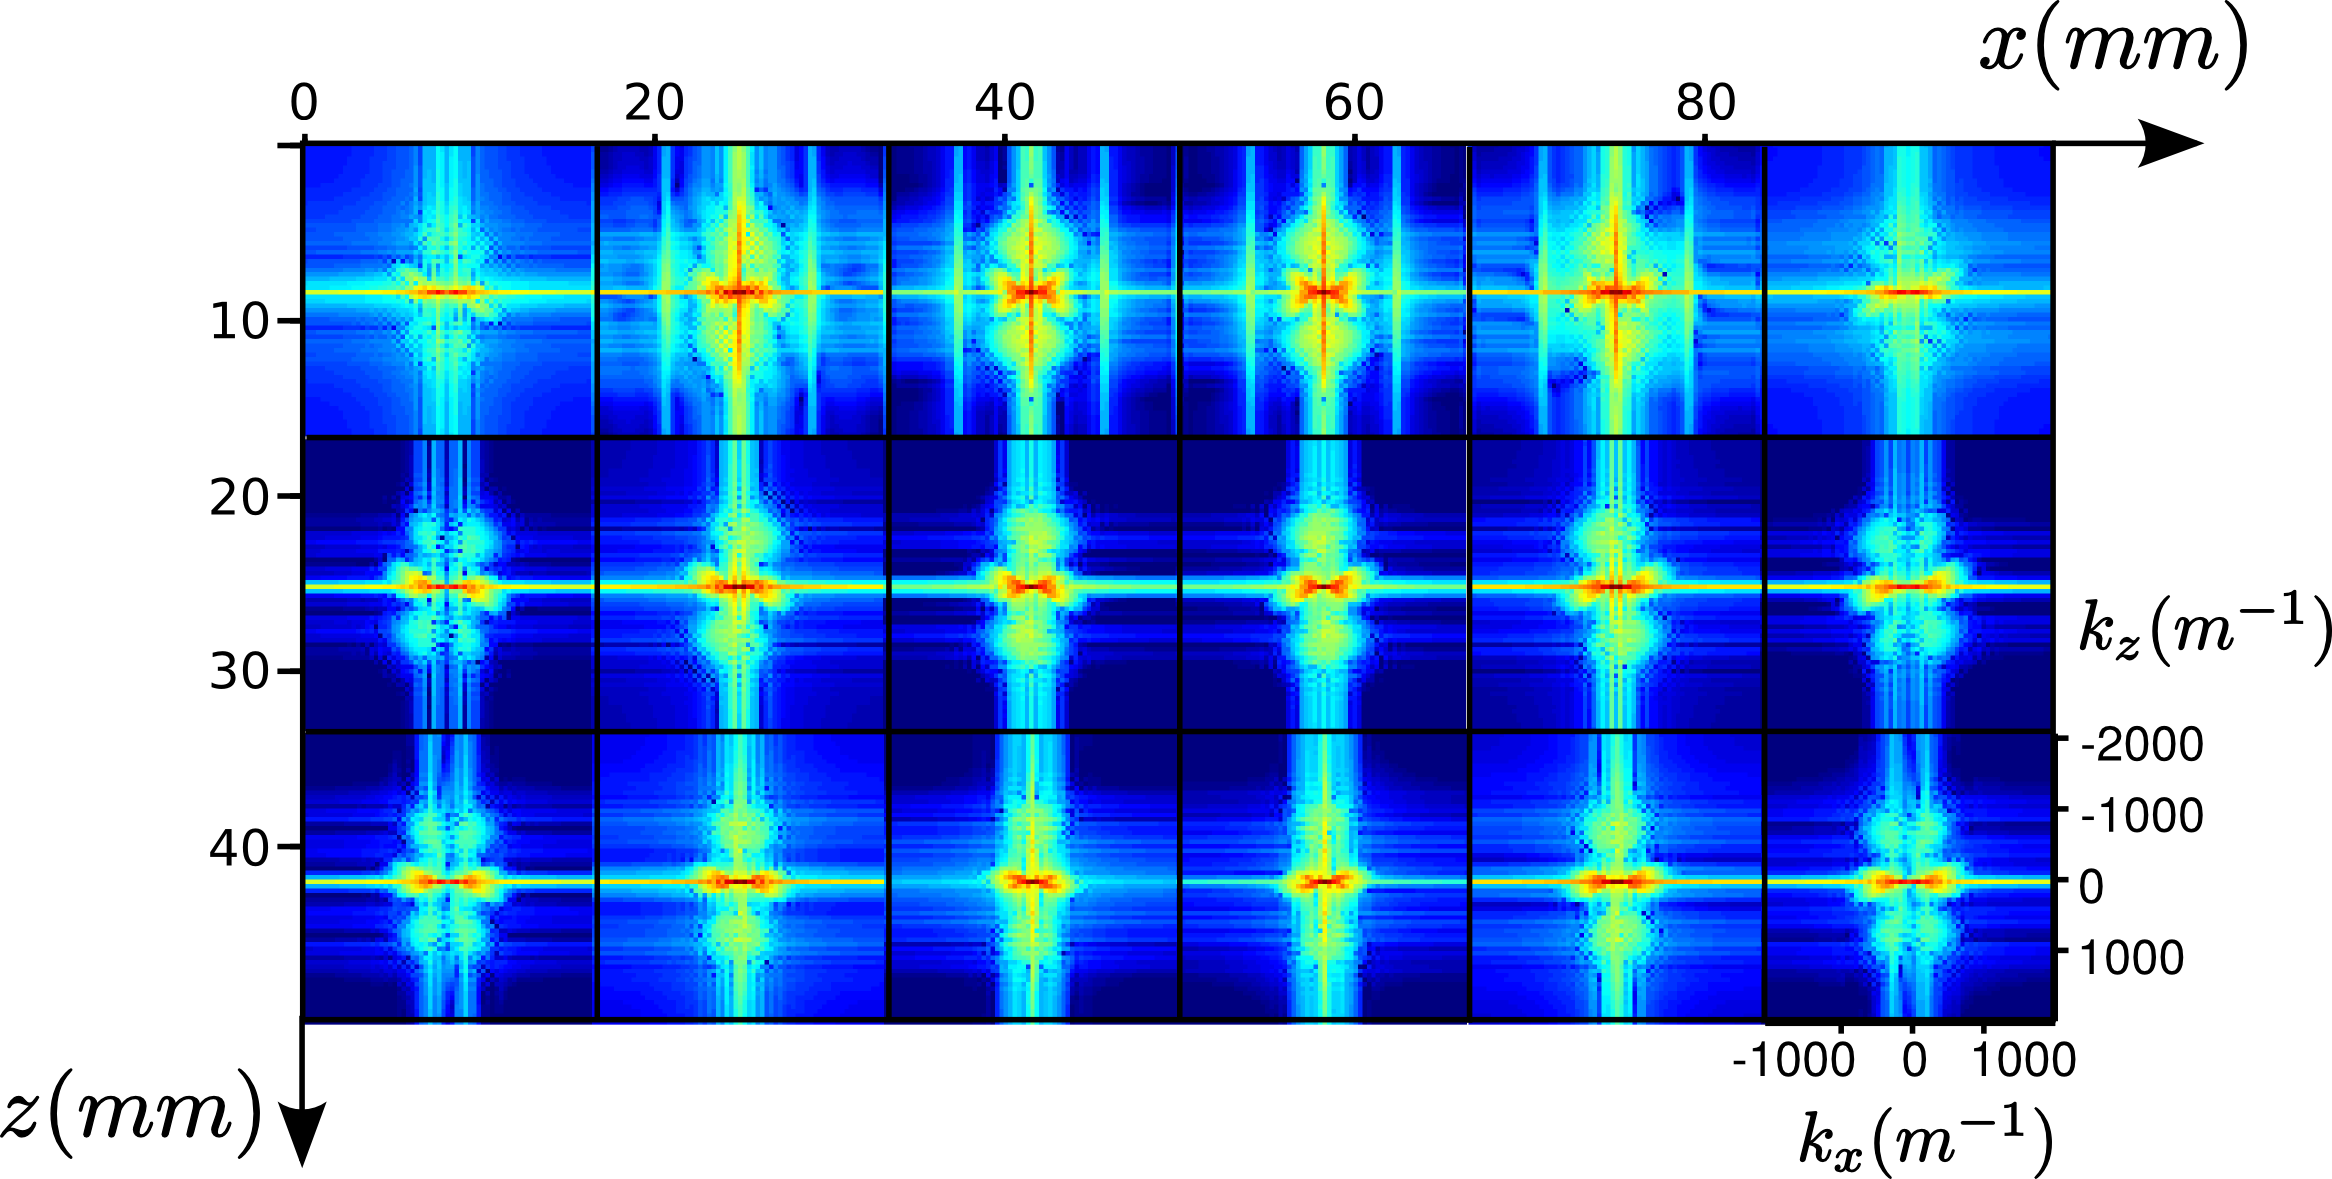
\includegraphics[height=3cm]{img/4200pt.png}\\
			\small{Pour 5 réflexions}\\[0.3cm]
			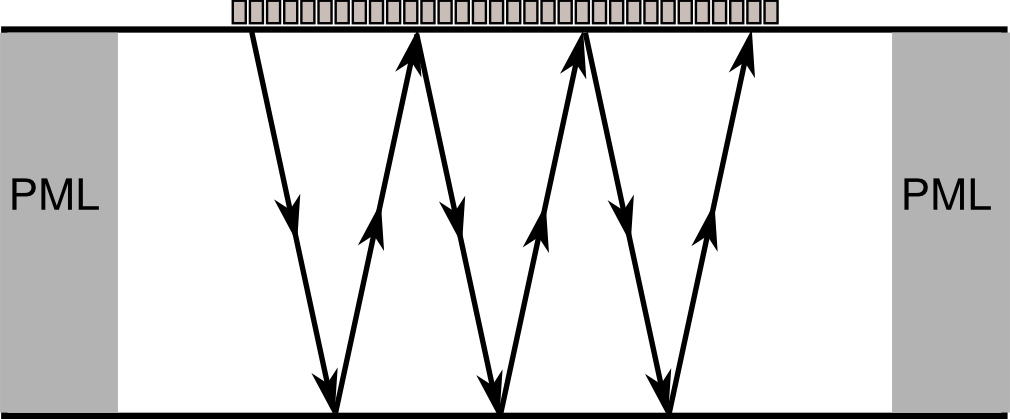
\includegraphics[height=1cm]{img/6ref.png}
		\end{figure}
	\end{columns}

\end{frame}

\section{Inversions en milieu isotrope}
\subsection*{}
\begin{frame}{\insertsectionhead}
	\begin{itemize}
		\item<1-> Milieu 2D, isotrope, acoustique
		\item<1-> Paramétrisation : vitesse + masse volumique
		\item<2-> Excitation : Ricker centré à 2 MHz 
	\end{itemize}	
	\only<1-1>{
	\begin{columns}
		\column{0.5\textwidth}
		\begin{figure}
			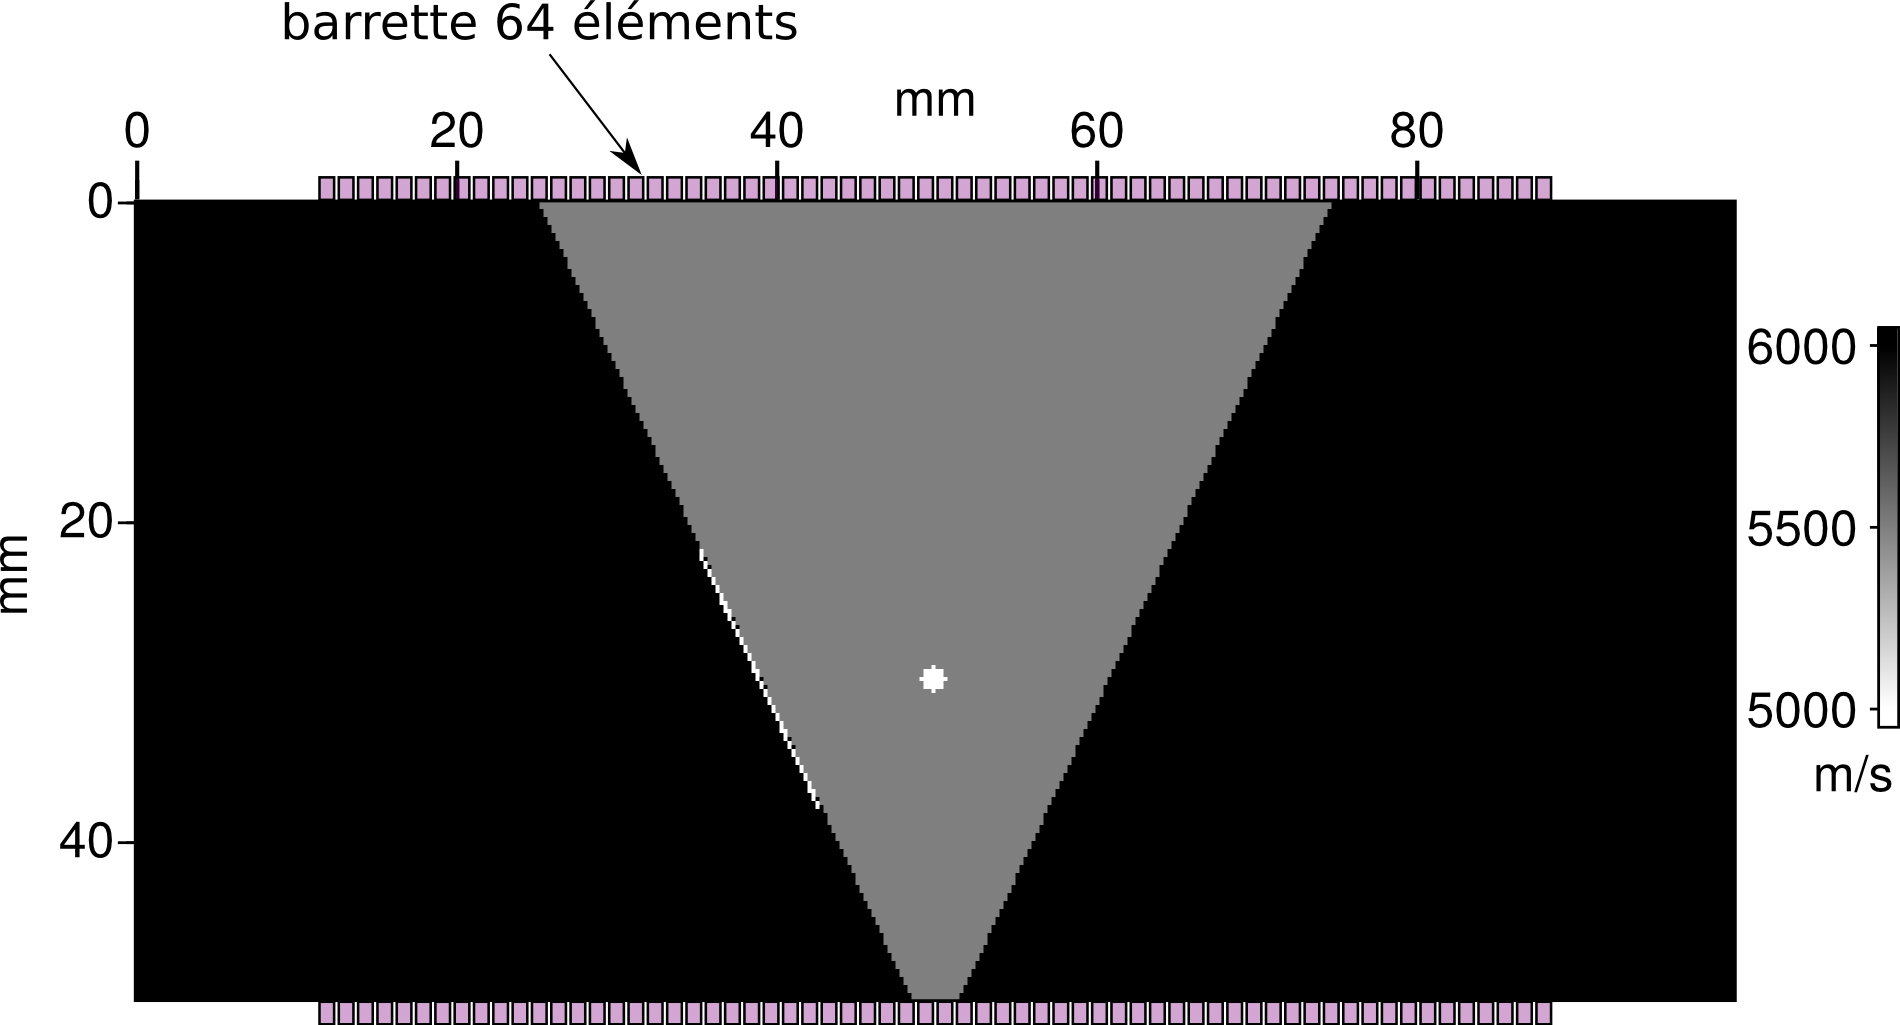
\includegraphics[width=\textwidth]{img/vp_true.png}\\
			{\small Vitesse vraie}
		\end{figure}
		\column{0.5\textwidth}
		\begin{figure}
			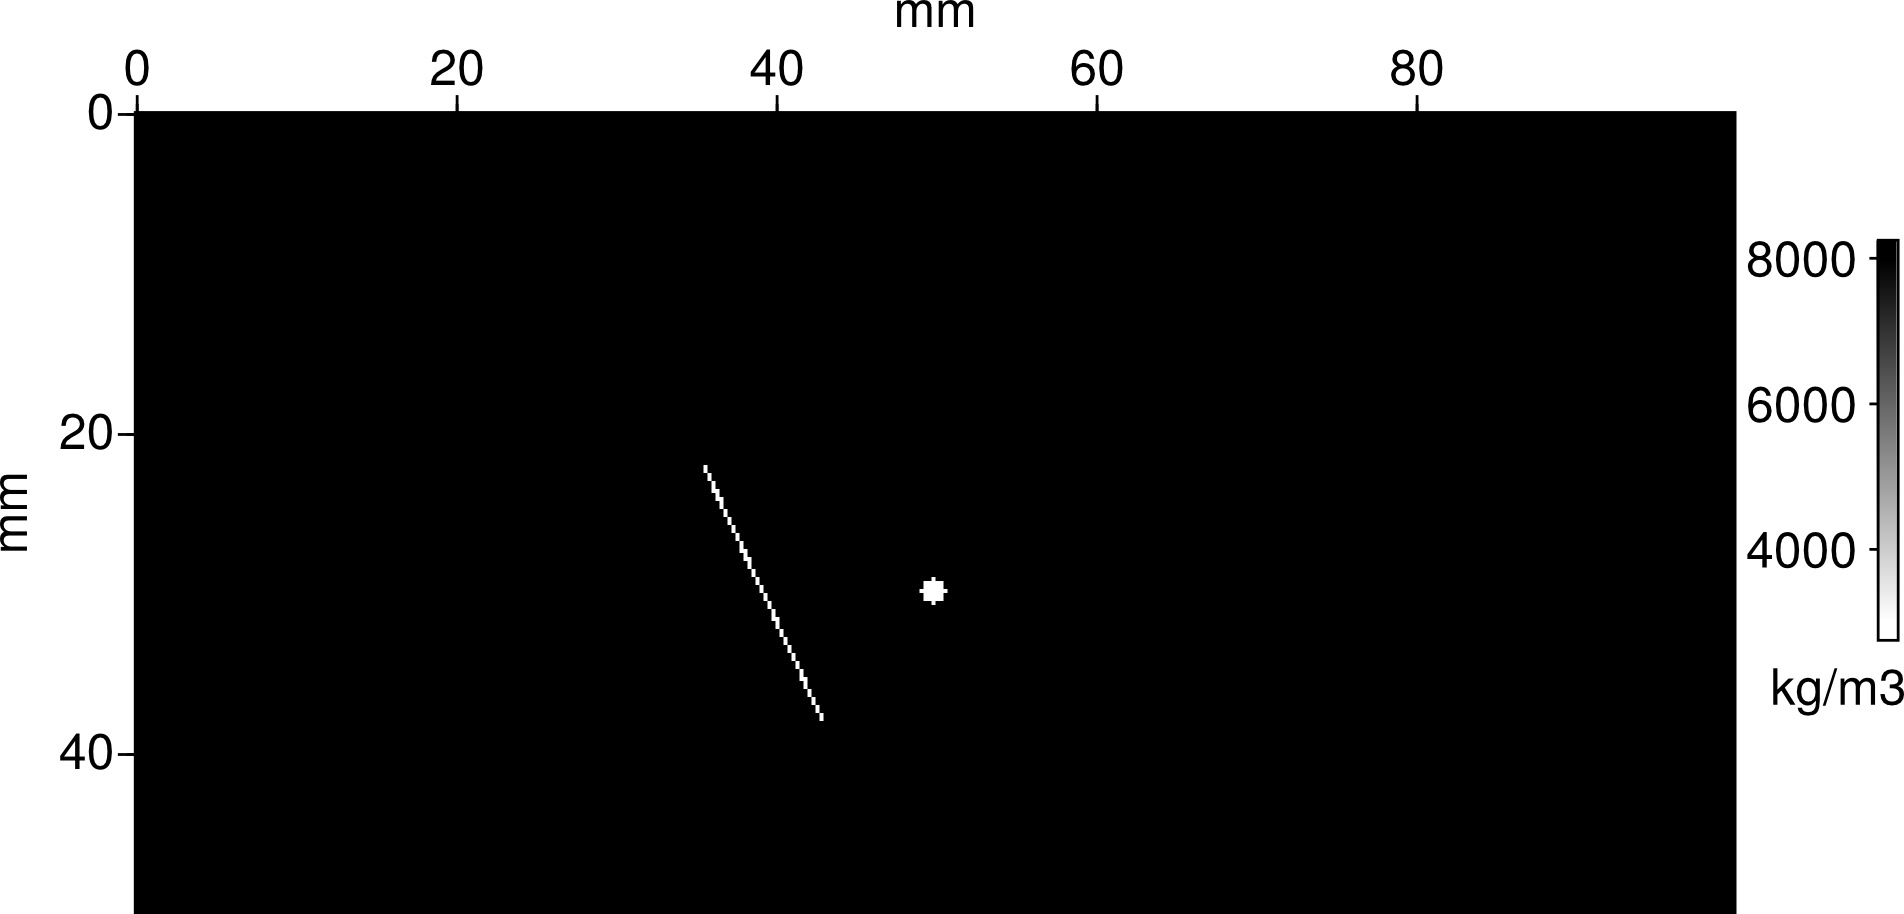
\includegraphics[width=\textwidth]{img/rho_true.png}\\
			{\small Masse volumique vraie}
		\end{figure}
	\end{columns}
	}
	
	\only<2->{
	\begin{columns}
		\column{0.5\textwidth}
		\begin{figure}
			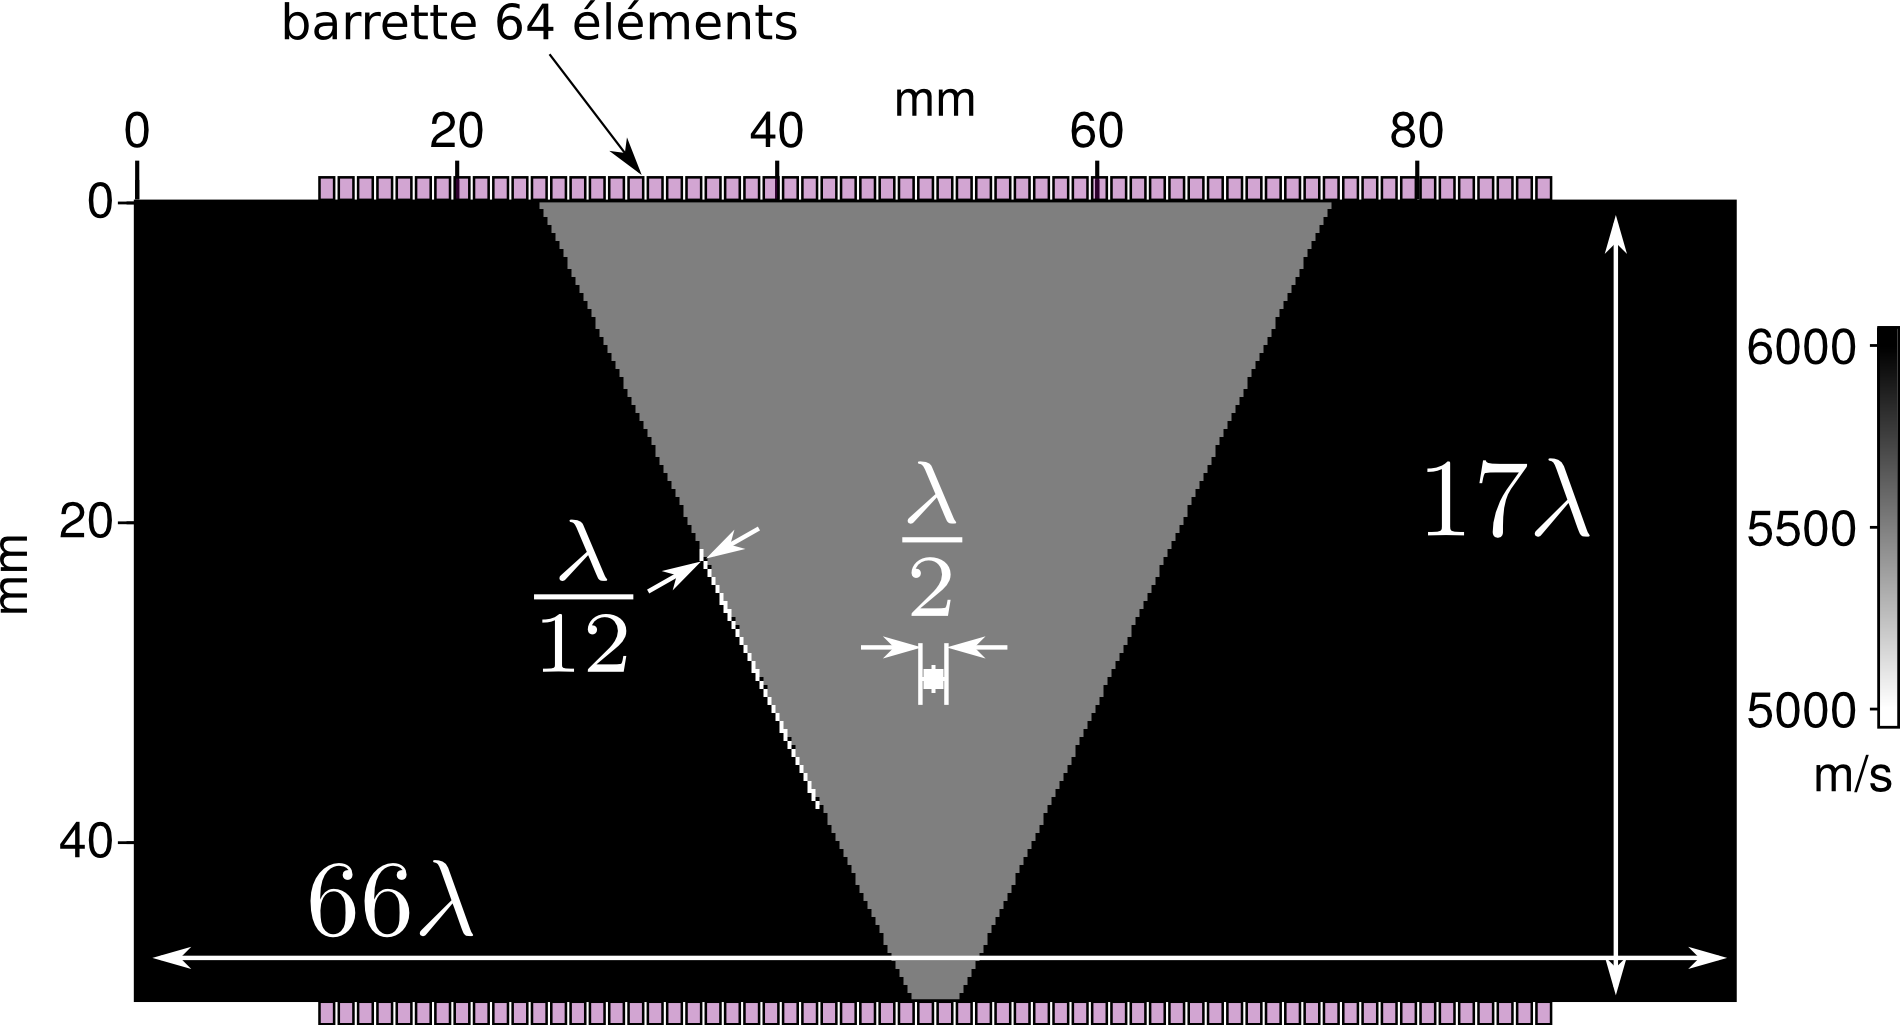
\includegraphics[width=\textwidth]{img/vp_true_lambda.png}\\
			{\small Vitesse vraie}
		\end{figure}
		\column{0.5\textwidth}
		\begin{figure}
			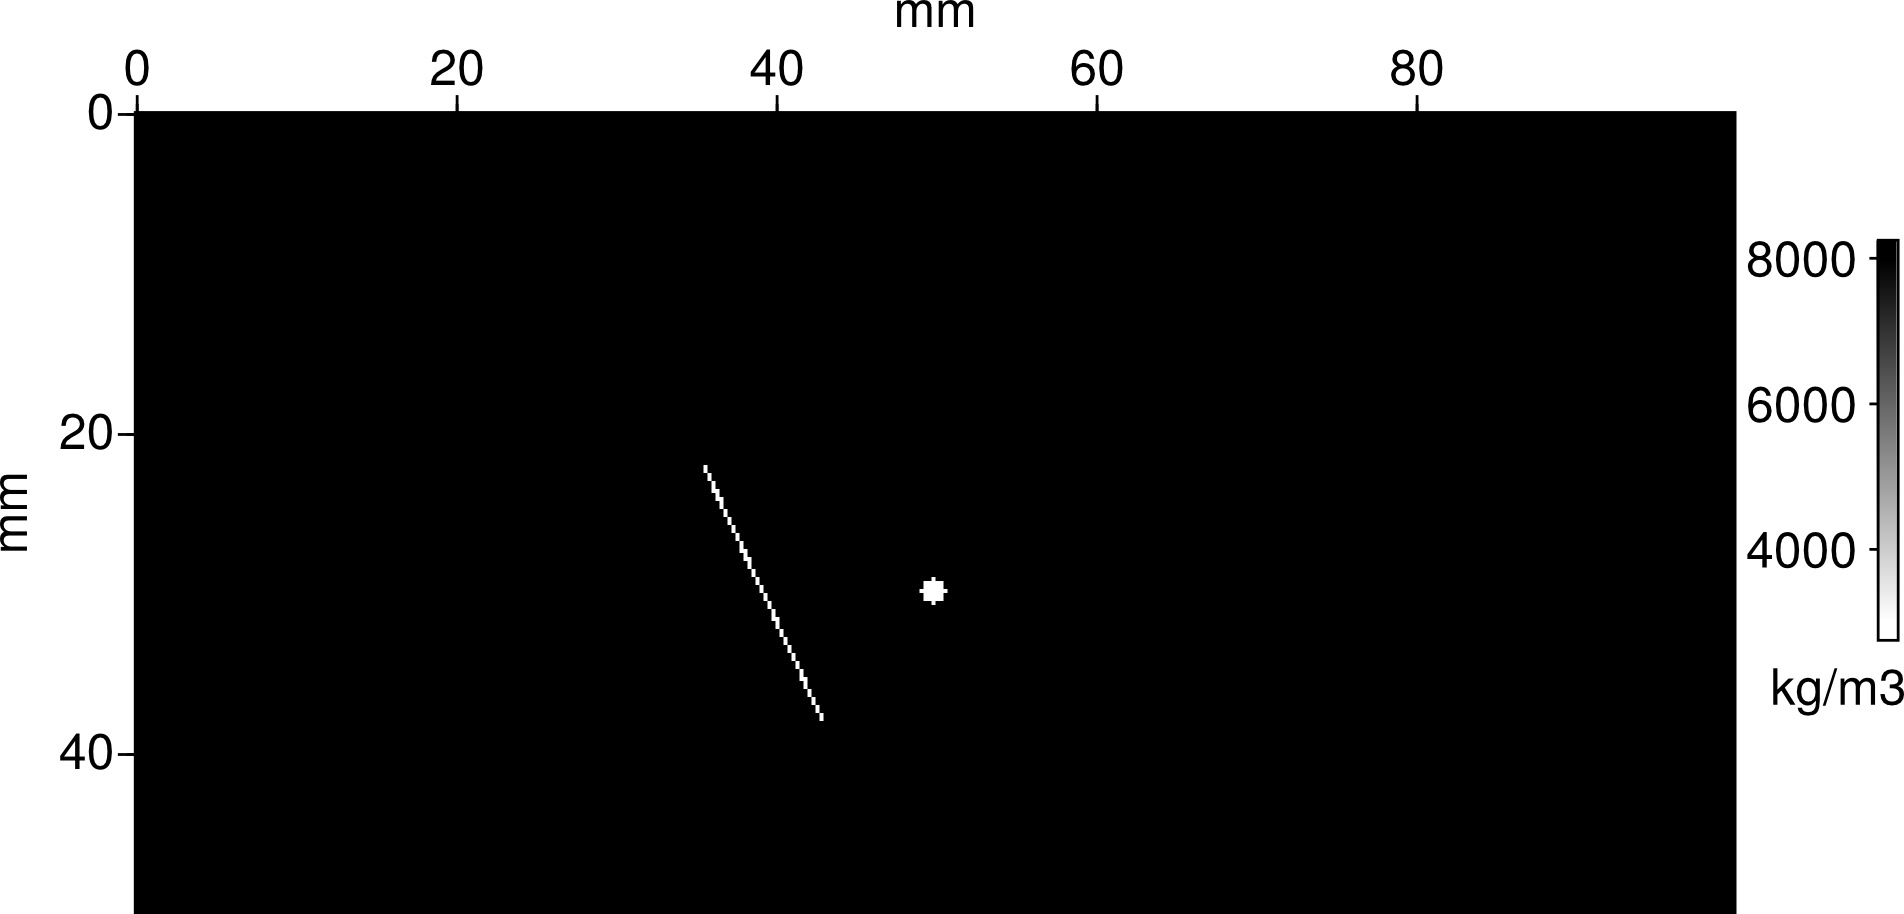
\includegraphics[width=\textwidth]{img/rho_true.png}\\
			{\small Masse volumique vraie}
		\end{figure}
	\end{columns}
	}
	
%	\vspace{1cm}
%	\begin{itemize}
%		\item 9 inversions successives de 200 kHz à 3 MHz pour
%			\begin{itemize}
%				\item mieux contraindre le problème
%				\item lever les ambiguïtés de déphasage 
%			\end{itemize}
%	\end{itemize}


\only<2->{
\begin{picture}(0,0)(0,0)\put(220,110){	
	\begin{tikzpicture}
			\node (a) at (0,0) {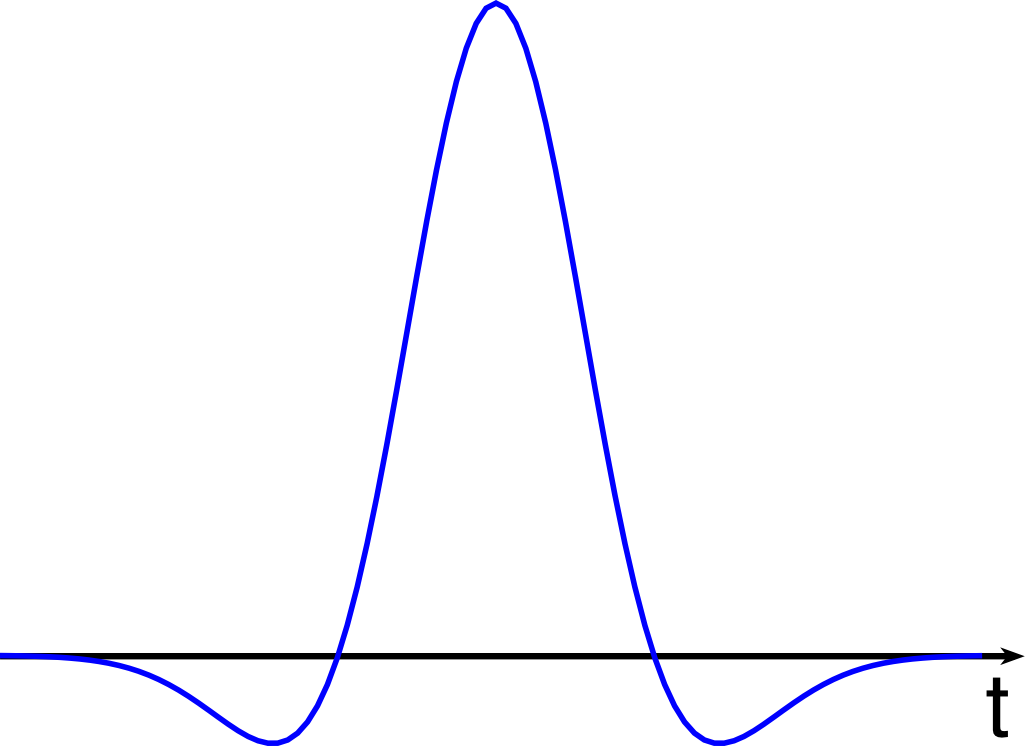
\includegraphics[height=1.5cm]{img/ricker.png}};
			\node (b) [below=-0cm of a] {\scriptsize Ondelette de Ricker};
	\end{tikzpicture}
}\end{picture}}
\end{frame}

\subsection{Stratégies d'inversion}
\begin{frame}{\insertsubsectionhead}
\begin{small}
	\begin{columns}
	\column{0.6\textwidth}
	\begin{itemize}
		\item pour contraindre le problème,  lever les ambiguïtés de phase
	\end{itemize}
	\onslide<2->{2 critères hiérarchiques :}
	\begin{itemize}
		\item<2-> influence des paramètres sur les données %(cinématique, dynamique, prépondérance, ...) %Fort lissage de $\bm{\Delta m}$ : gaussien sur 2 $\lambda$
		\item<4-> contenu fréquentiel
	\end{itemize}
	\column{0.5\textwidth}
		\centering
		\vspace{-0.5cm}
		\only<3-4>{
		\includegraphics[height=2.7cm]{img/vp_smooth/vp_smooth.png}\\
		\scriptsize{~~}\\
		}
		\only<5-5>{
		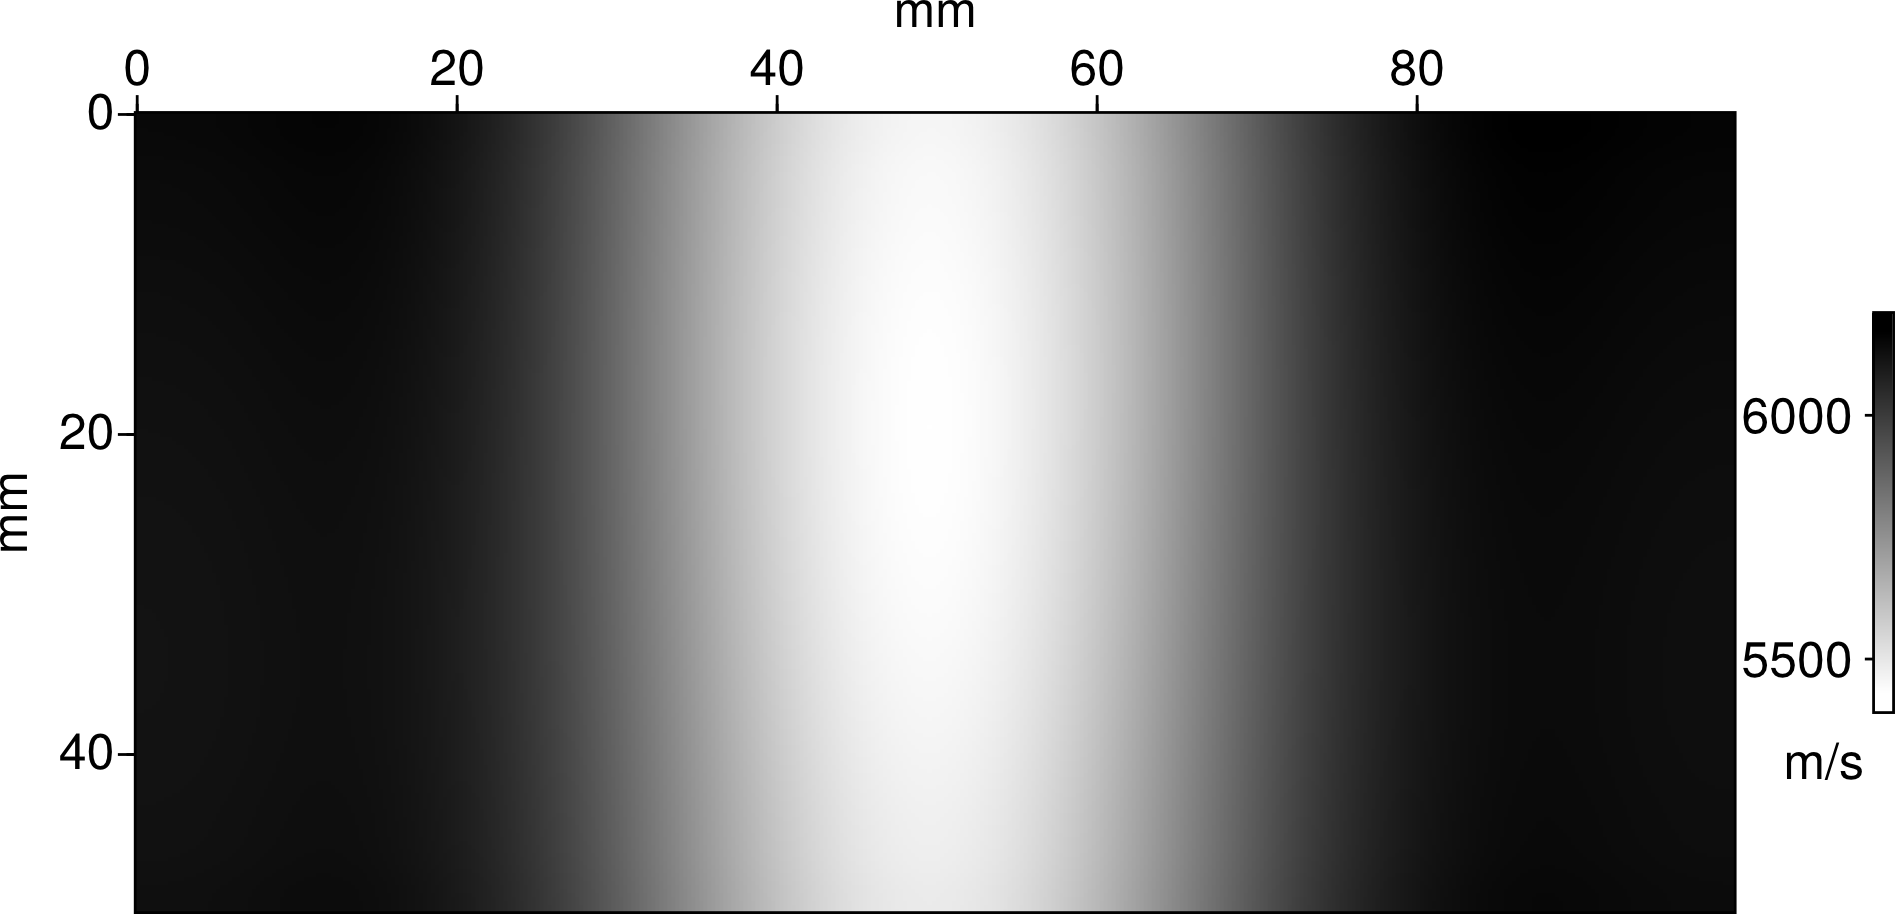
\includegraphics[height=2.7cm]{img/vp_smooth/vp_200k.png}\\
		\scriptsize{f$\sim$ 200 kHz}\\
		}
		\only<6-6>{
		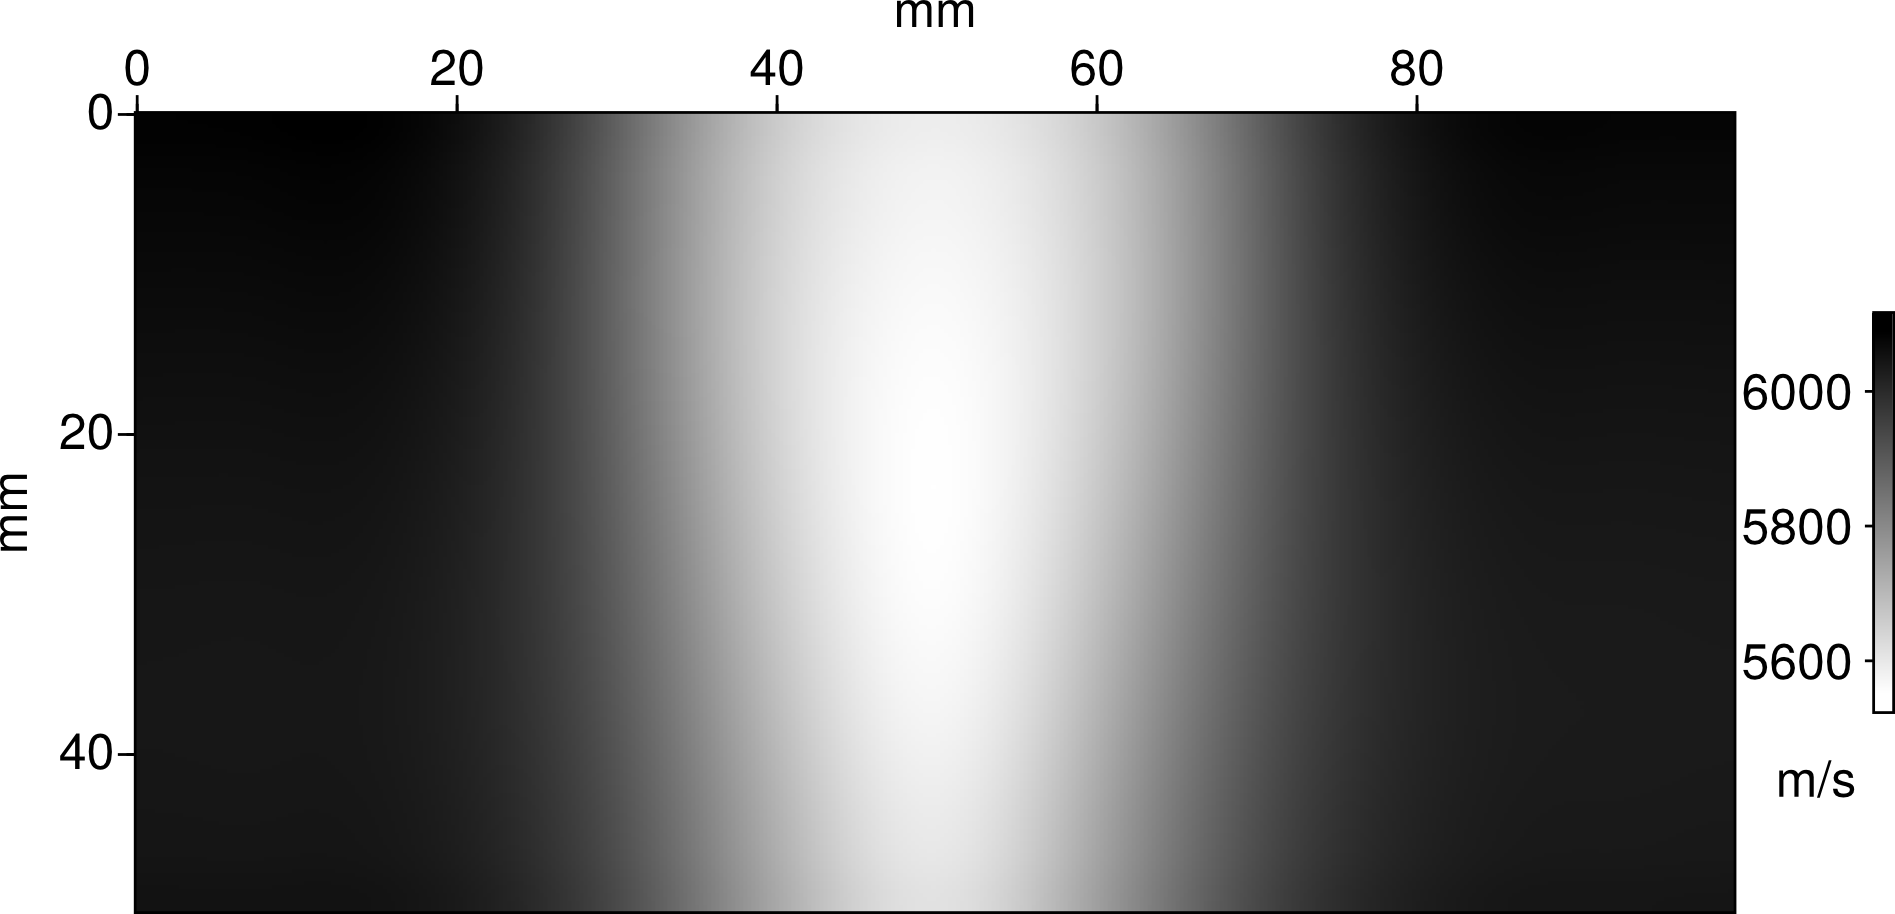
\includegraphics[height=2.7cm]{img/vp_smooth/vp_300k.png}\\
		\scriptsize{f$\sim$ 300 kHz}\\
		}	
		\only<7-7>{
		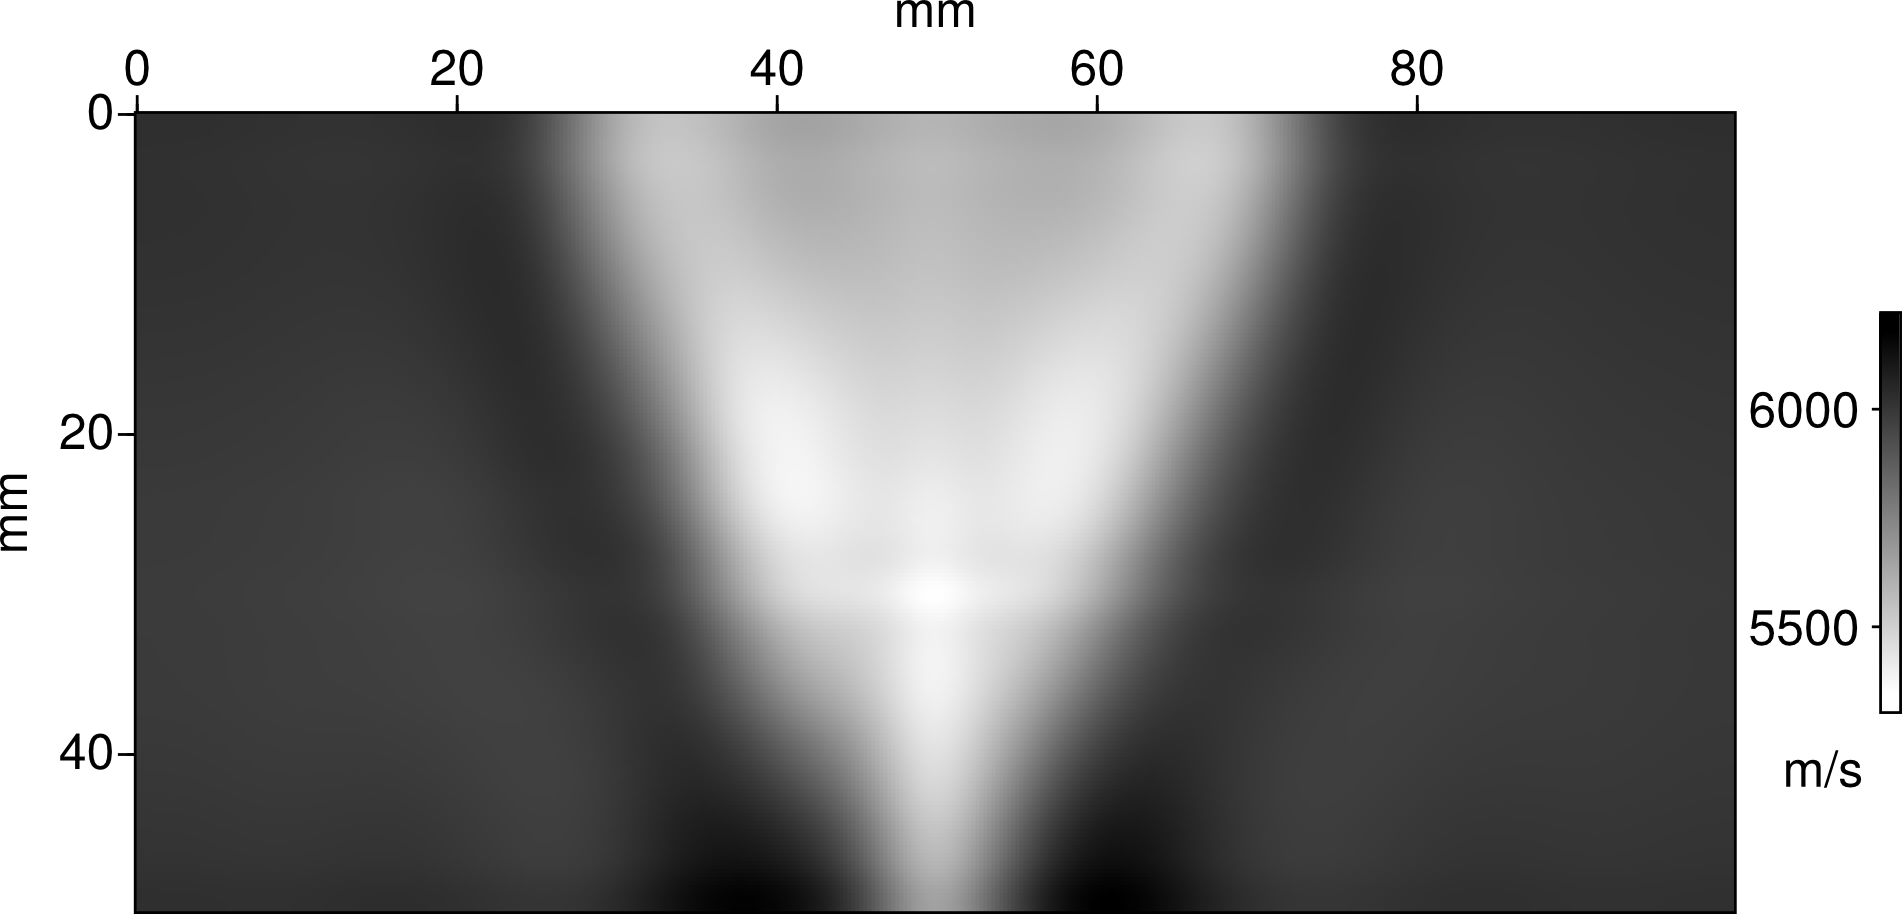
\includegraphics[height=2.7cm]{img/vp_smooth/vp_450k.png}\\
		\scriptsize{f$\sim$ 450 kHz}\\
		}
		\only<8-8>{
		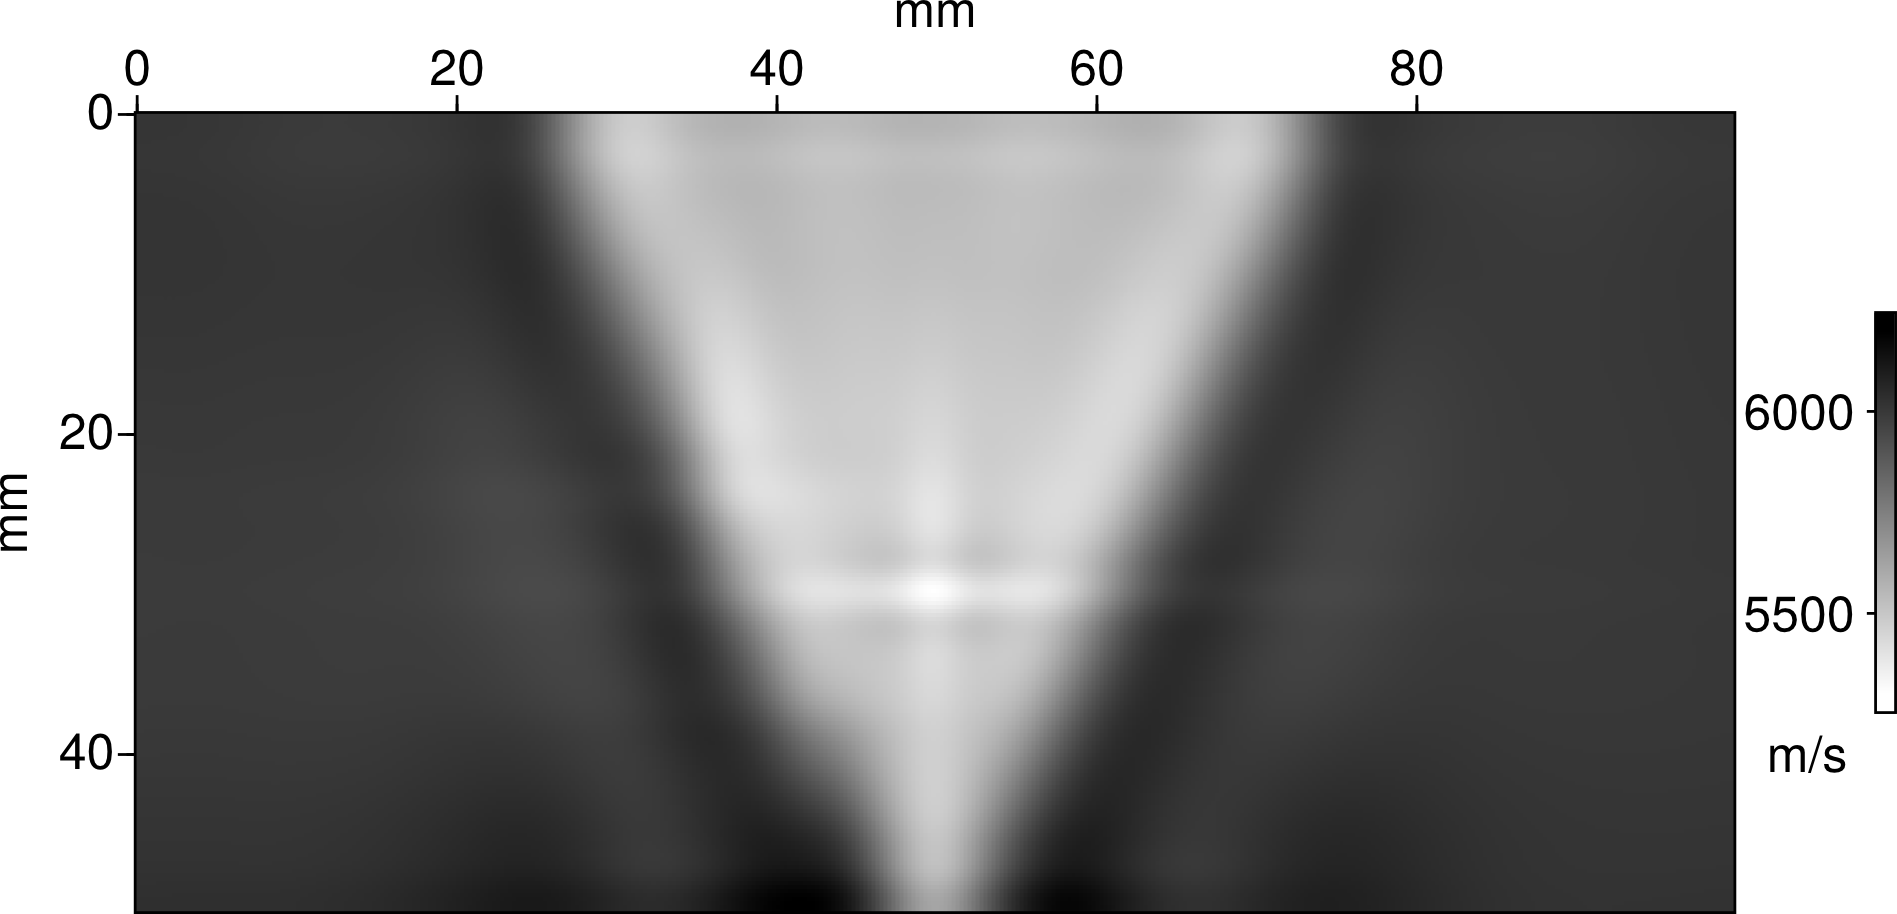
\includegraphics[height=2.7cm]{img/vp_smooth/vp_675k.png}\\
		\scriptsize{f$\sim$ 675 kHz}\\
		}
		\only<9-9>{
		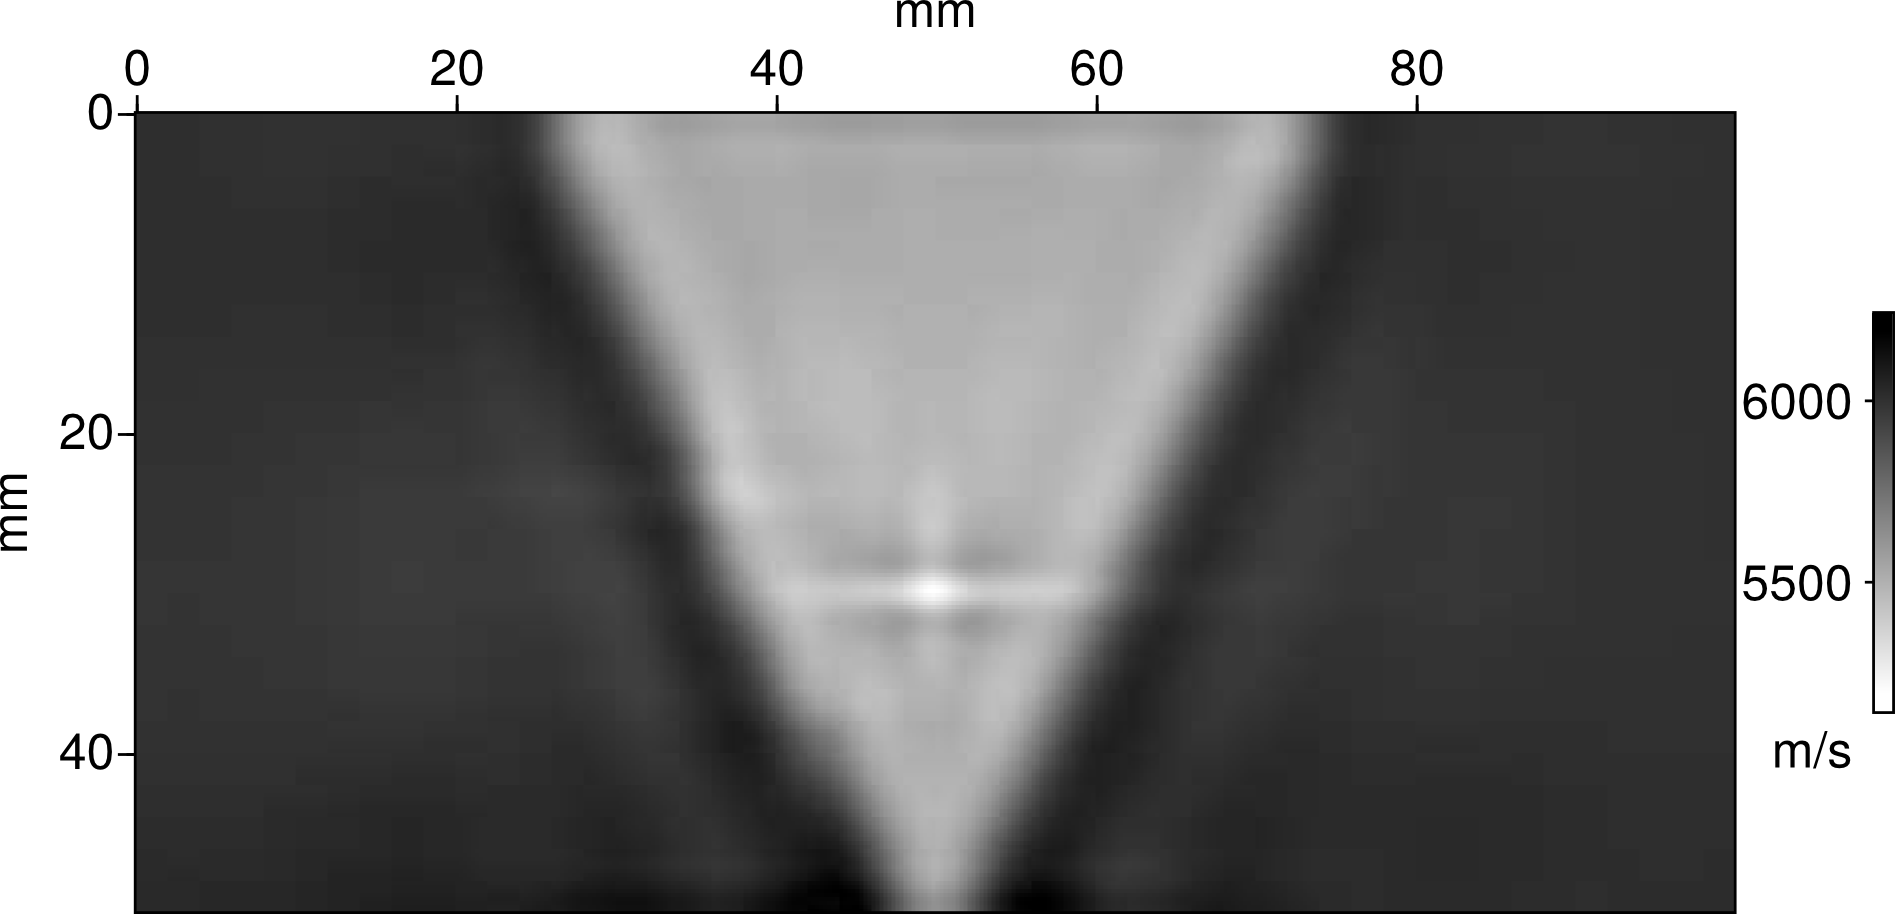
\includegraphics[height=2.7cm]{img/vp_smooth/vp_1000k.png}\\
		\scriptsize{f$\sim$ 1000 kHz}\\
		}
		\only<10-10>{
		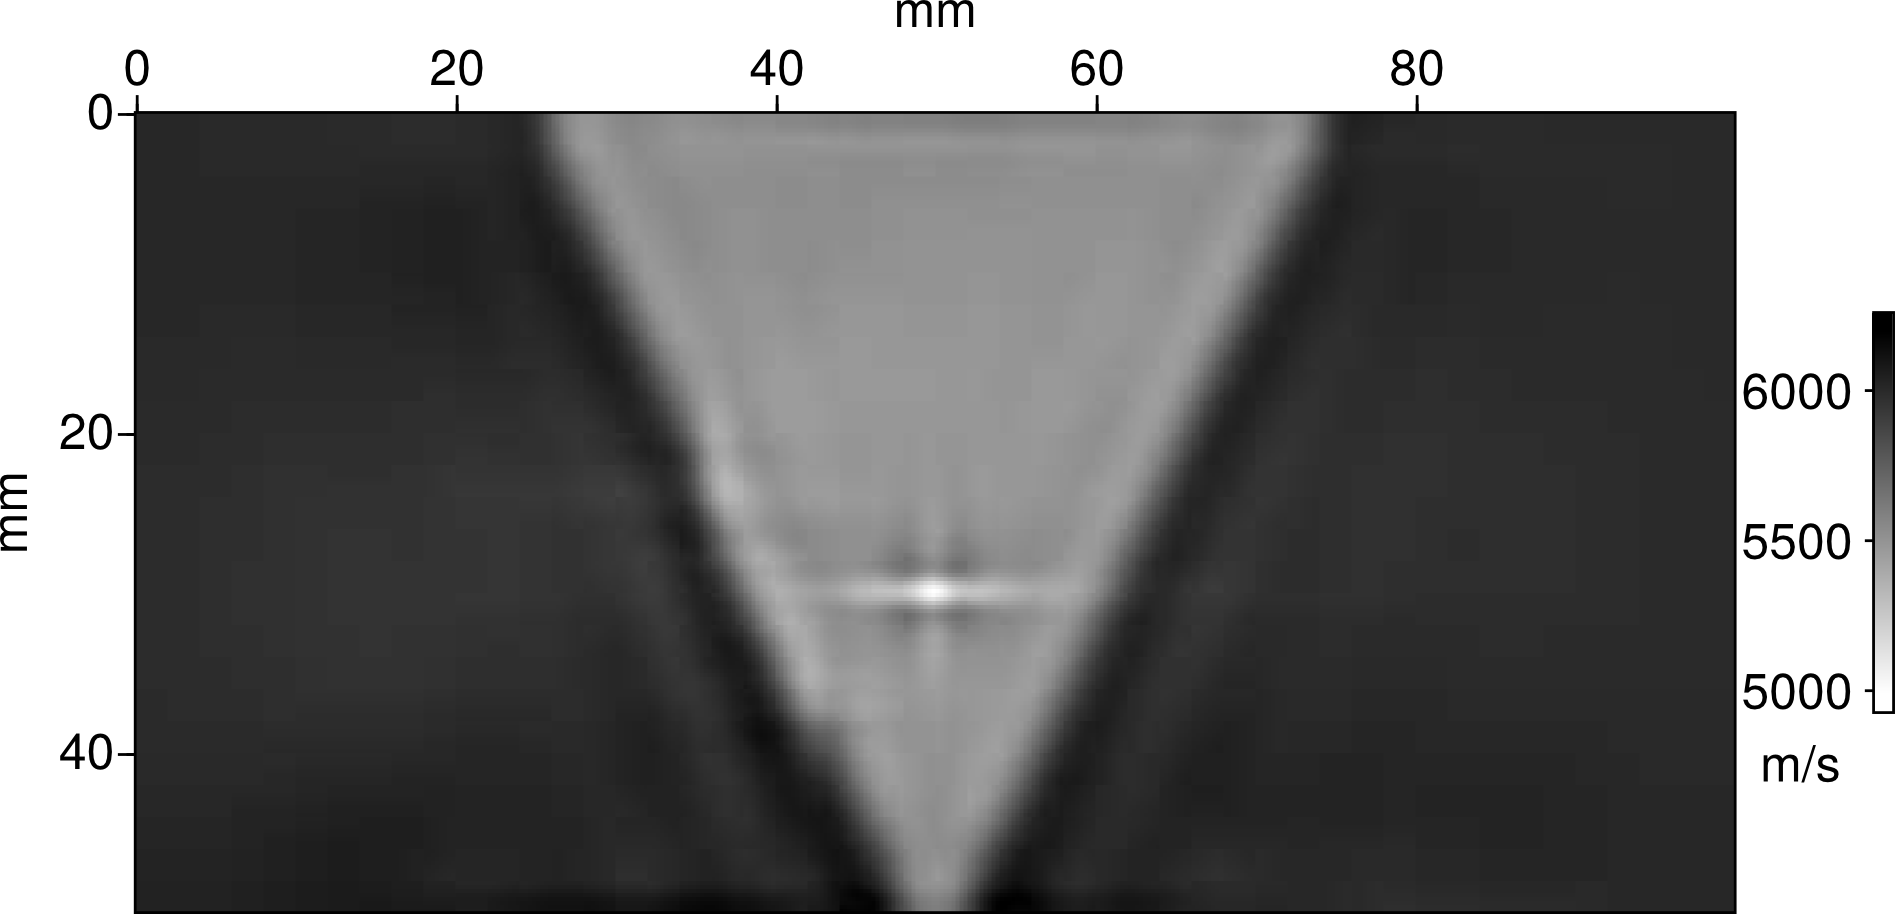
\includegraphics[height=2.7cm]{img/vp_smooth/vp_1500k.png}\\
		\scriptsize{f$\sim$ 1500 kHz}\\
		}
		\only<11->{
		\includegraphics[height=2.7cm]{img/vp_smooth/vp_smooth.png}\\
		\scriptsize{f$\sim$ 2200 kHz}\\
		}			
		\only<3->{\scriptsize{Construction d'un modèle de vitesse lissé}}
	\end{columns}
	\vspace{0.3cm}	
	\begin{columns}
		\column{0.3\textwidth}
		\onslide<2->{
		\centering
		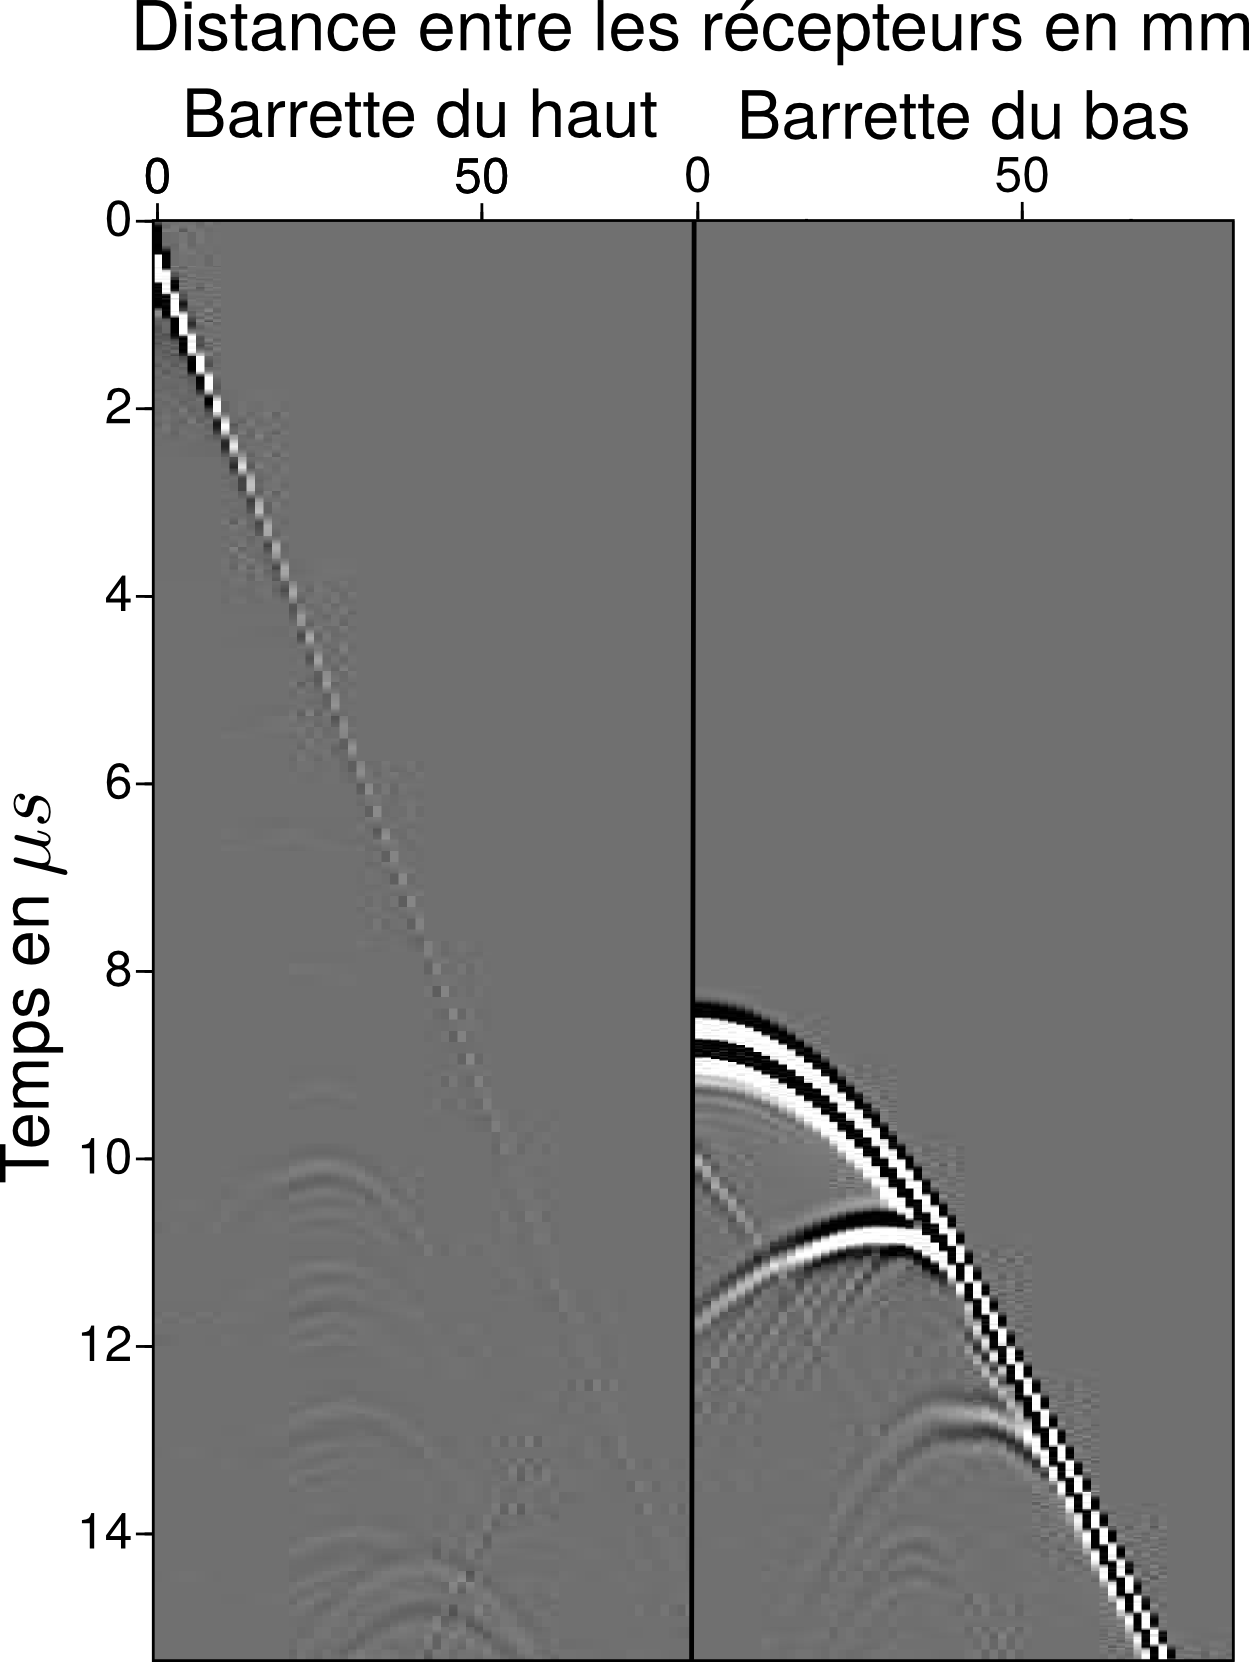
\includegraphics[height=4.3cm]{img/rho_mono/data_rho_uni.png}\\
		\scriptsize{Données issues d'une masse volumique homogène}
		\column{0.3\textwidth}
		\centering
		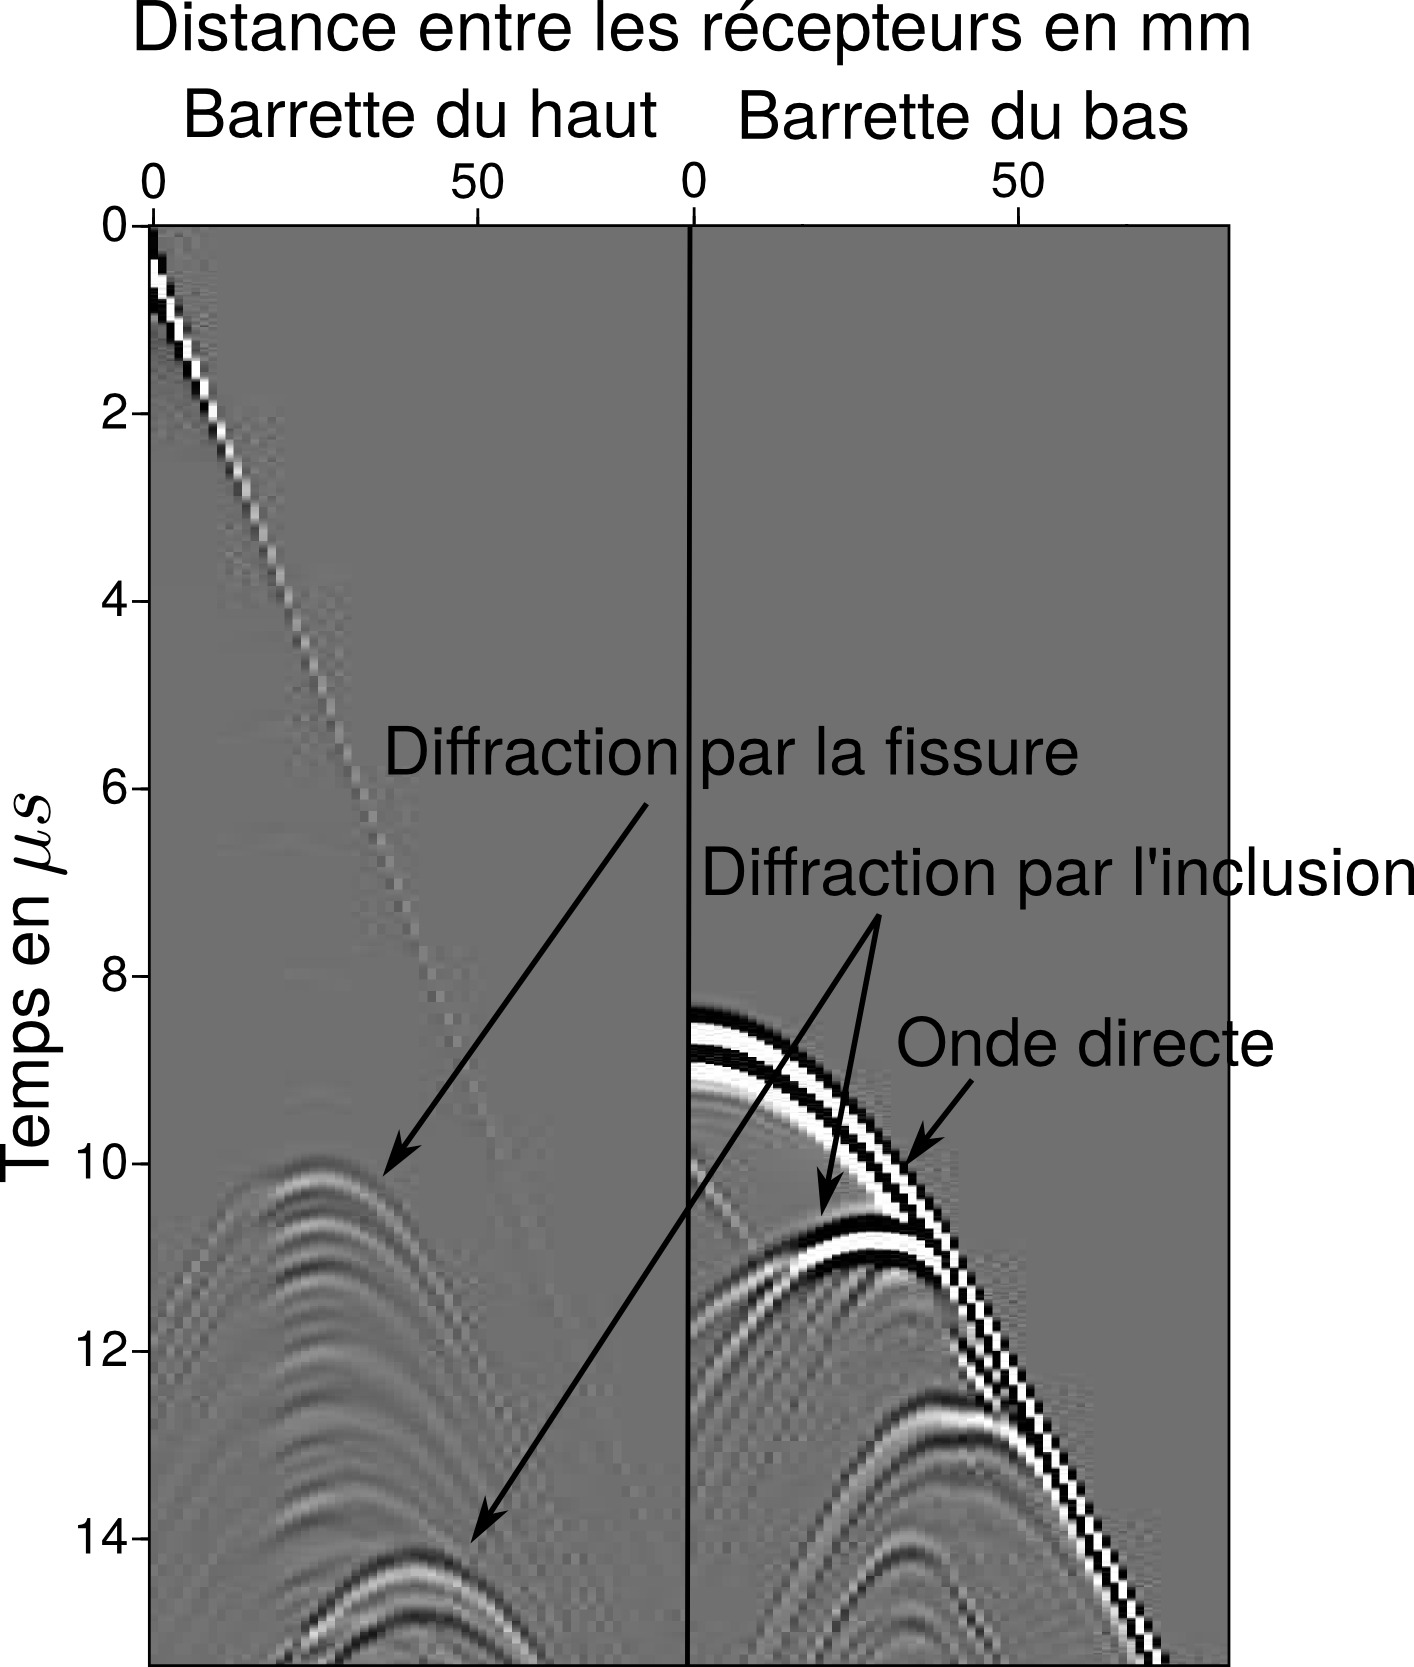
\includegraphics[height=4.3cm]{img/rho_mono/data_rho_vrai.png}\\
		\scriptsize{Données issues de la vraie masse volumique}
		}
	\end{columns}
	

\end{small}
\end{frame}

\begin{frame}{\insertsectionhead}
\setlength{\leftmargin}{-2cm}
\setlength{\rightmargin}{-2cm}
%\setlength{\textwidth}{29cm}
\begin{picture}(0,0)(0,0)\put(-20,-33){
	$v_{p}$
}\end{picture}
\begin{picture}(0,0)(0,0)\put(-20,-87){
	$\rho$
}\end{picture}
\vspace{-0.5cm}
\begin{itemize}
	\small{\item 9 inversions successives de 200 kHz à 3 MHz }\\[0.3cm]
\end{itemize}
\vspace{0.3cm}
	\begin{columns}
		\column{0.3\textwidth}
		\centering
		\scriptsize{Modèles initiaux}
		\includegraphics[height=1.9cm]{img/vp_mono_smooth/vp_smooth.png}\\
		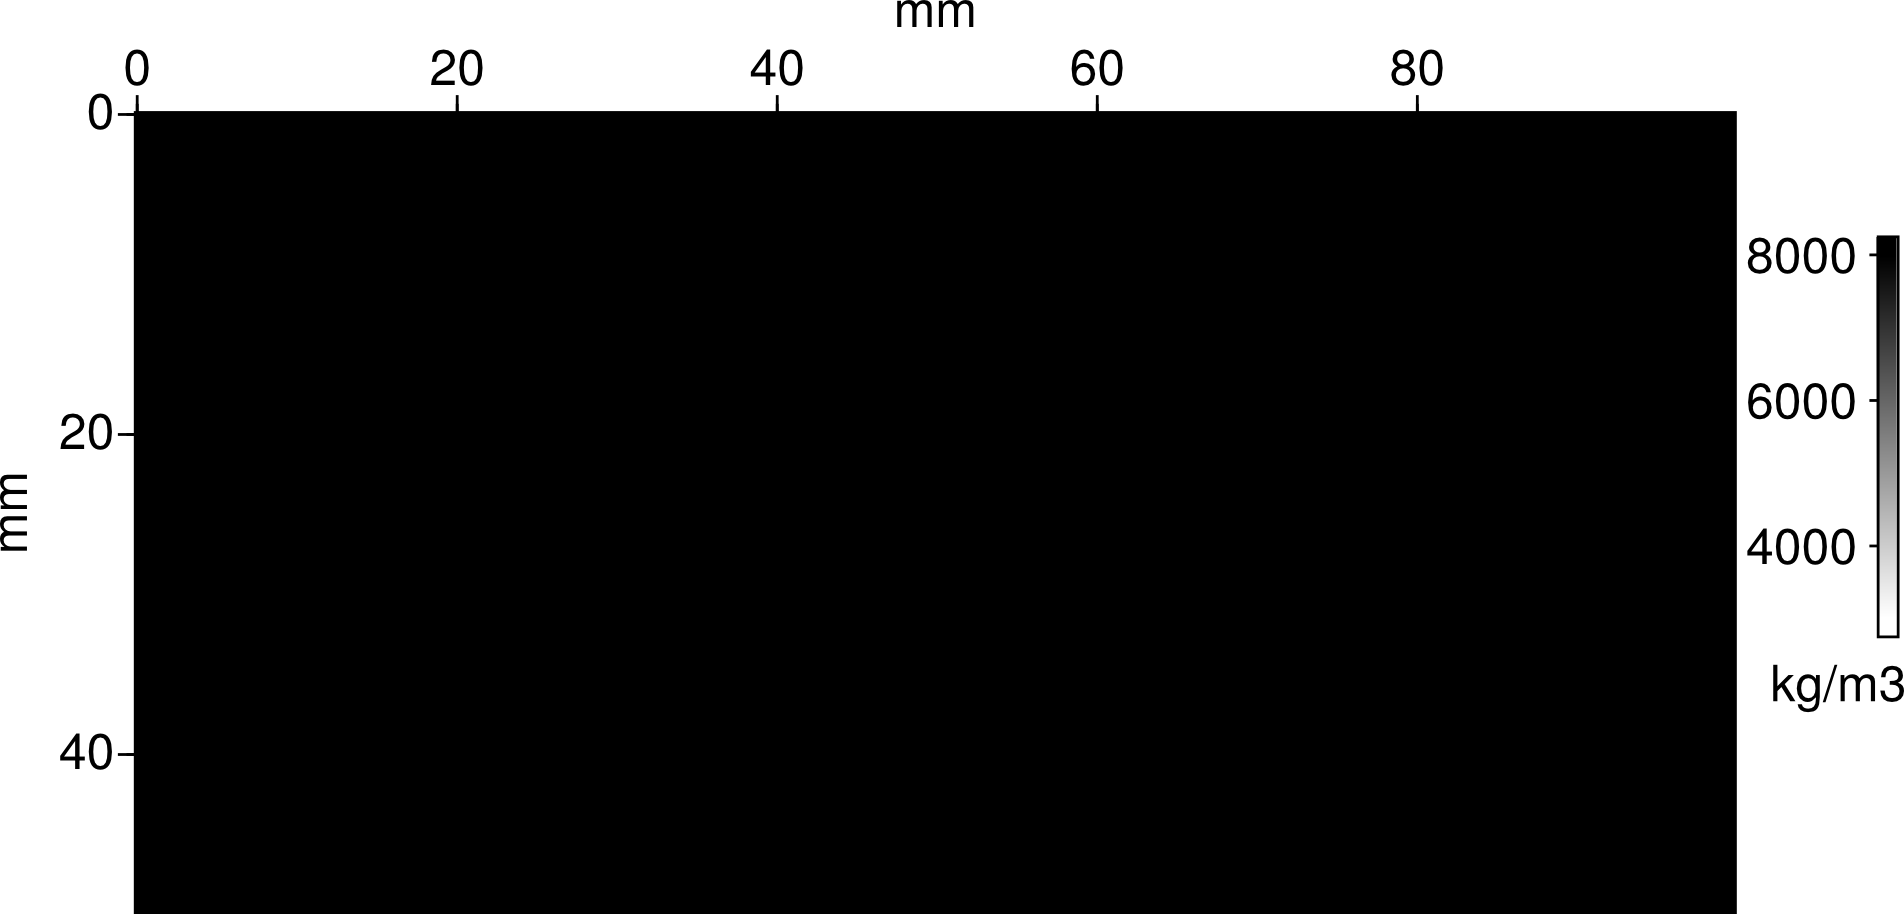
\includegraphics[height=1.9cm]{img/rho_mono/rho_init.png}		
		\column{0.3\textwidth}
		\centering
		\scriptsize{Inversions monoparamètres}
		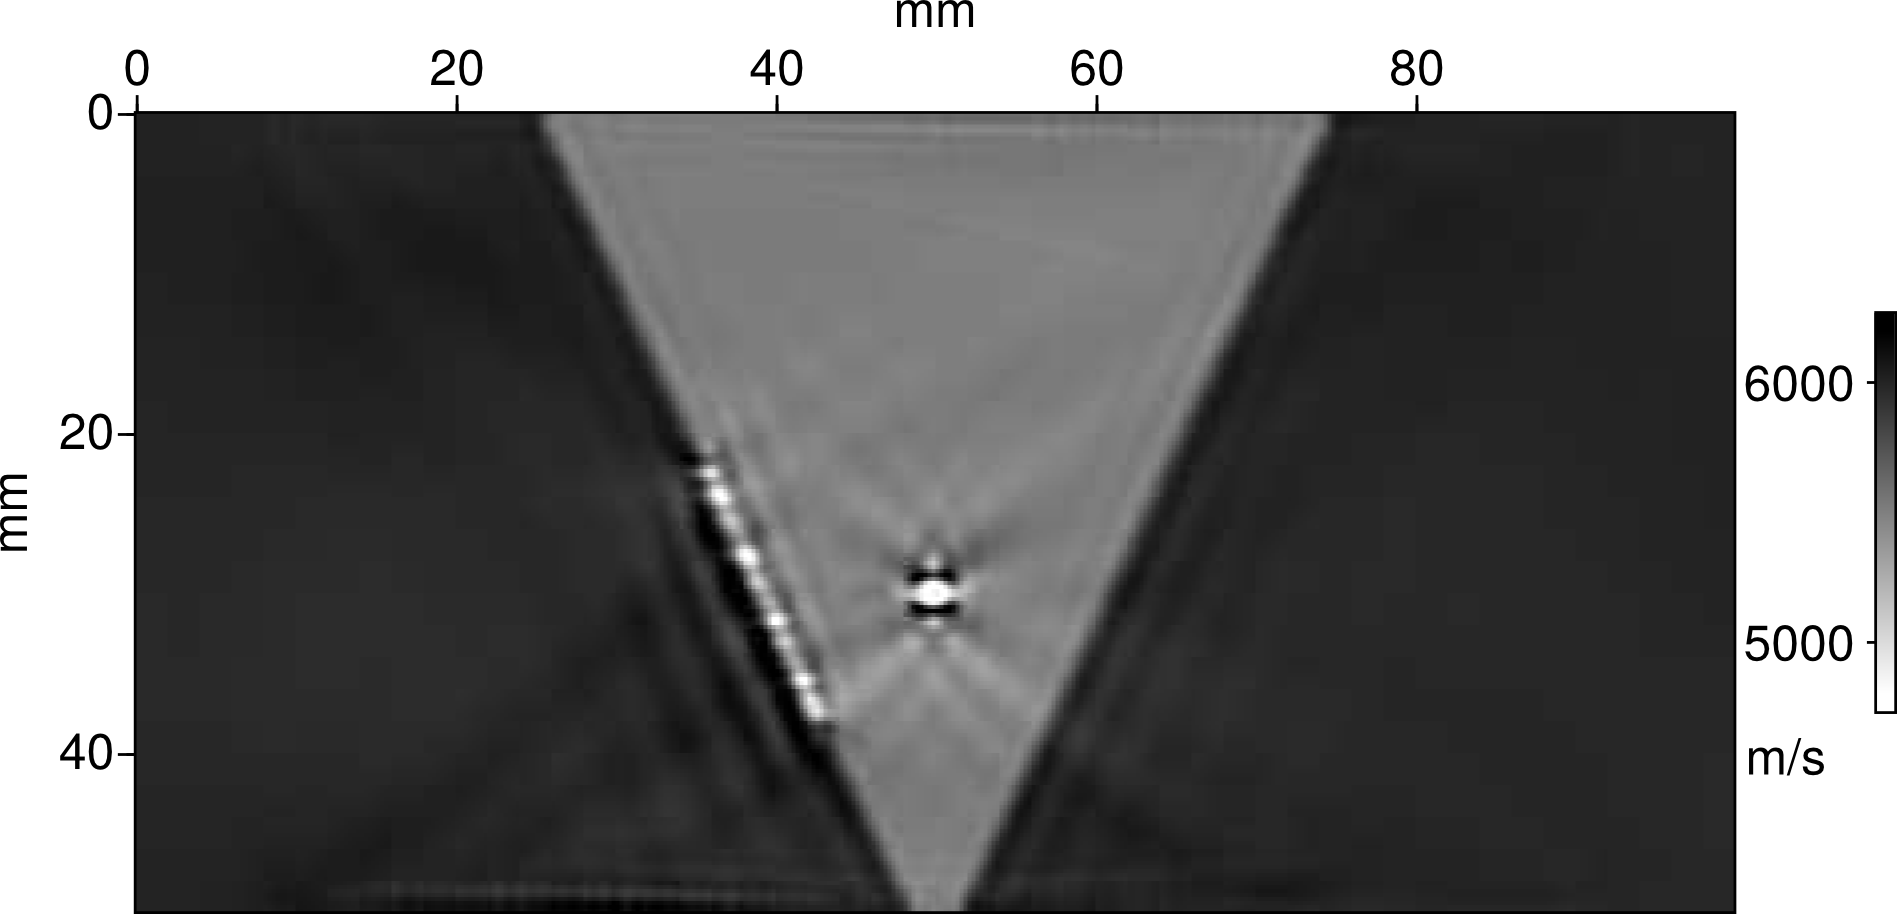
\includegraphics[height=1.9cm]{img/vp_mono_uni/vp_3300k.png}\\
		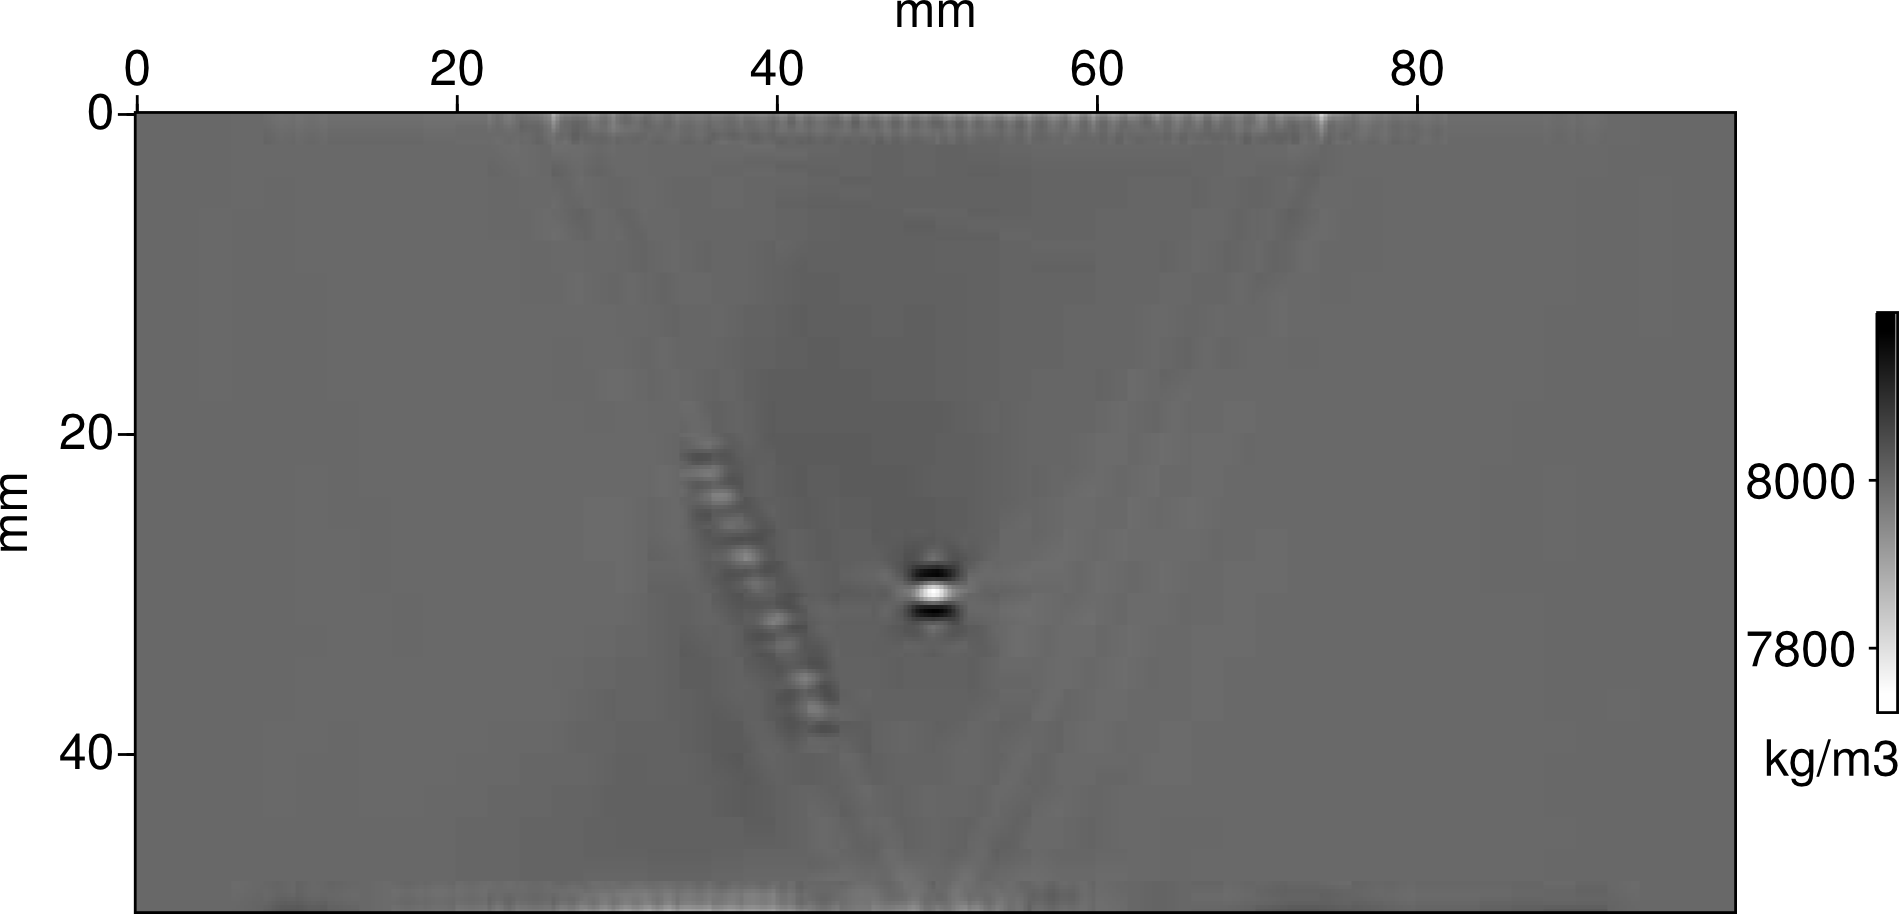
\includegraphics[height=1.9cm]{img/rho_mono/rho_mono.png}		
		\column{0.3\textwidth}
		\centering
		\scriptsize{Inversion multiparamètre}
		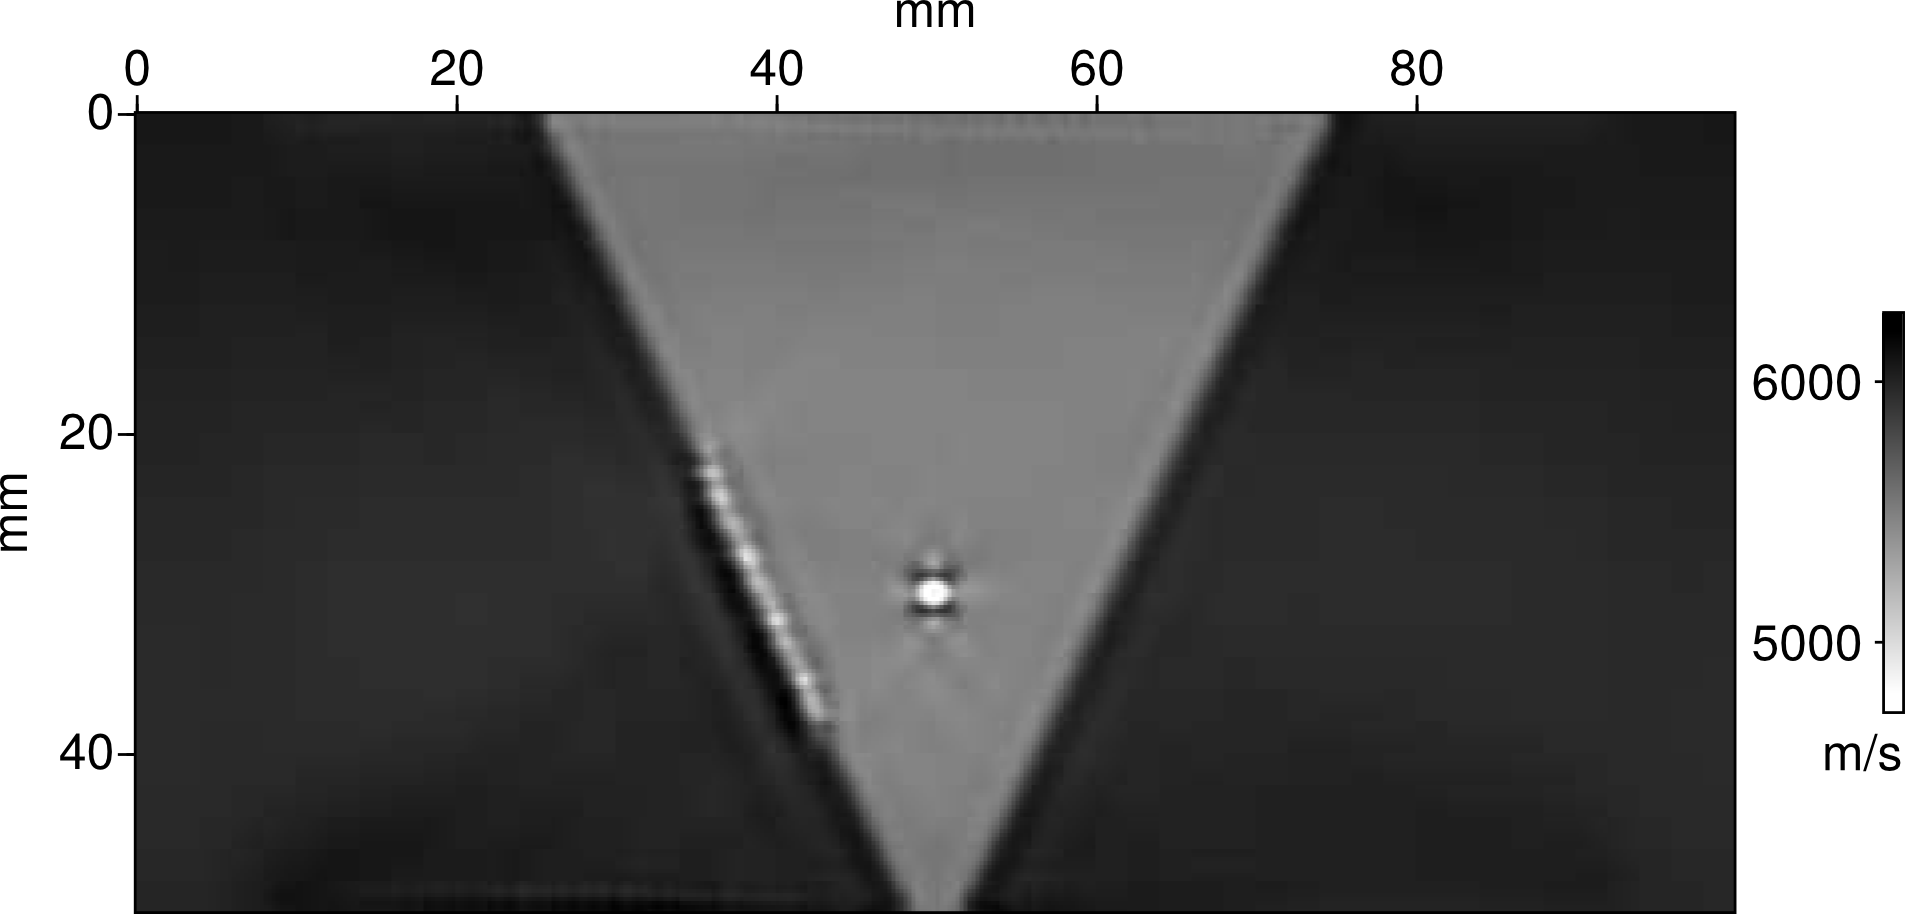
\includegraphics[height=1.9cm]{img/multi/vp_multi_6000k.png}\\		
		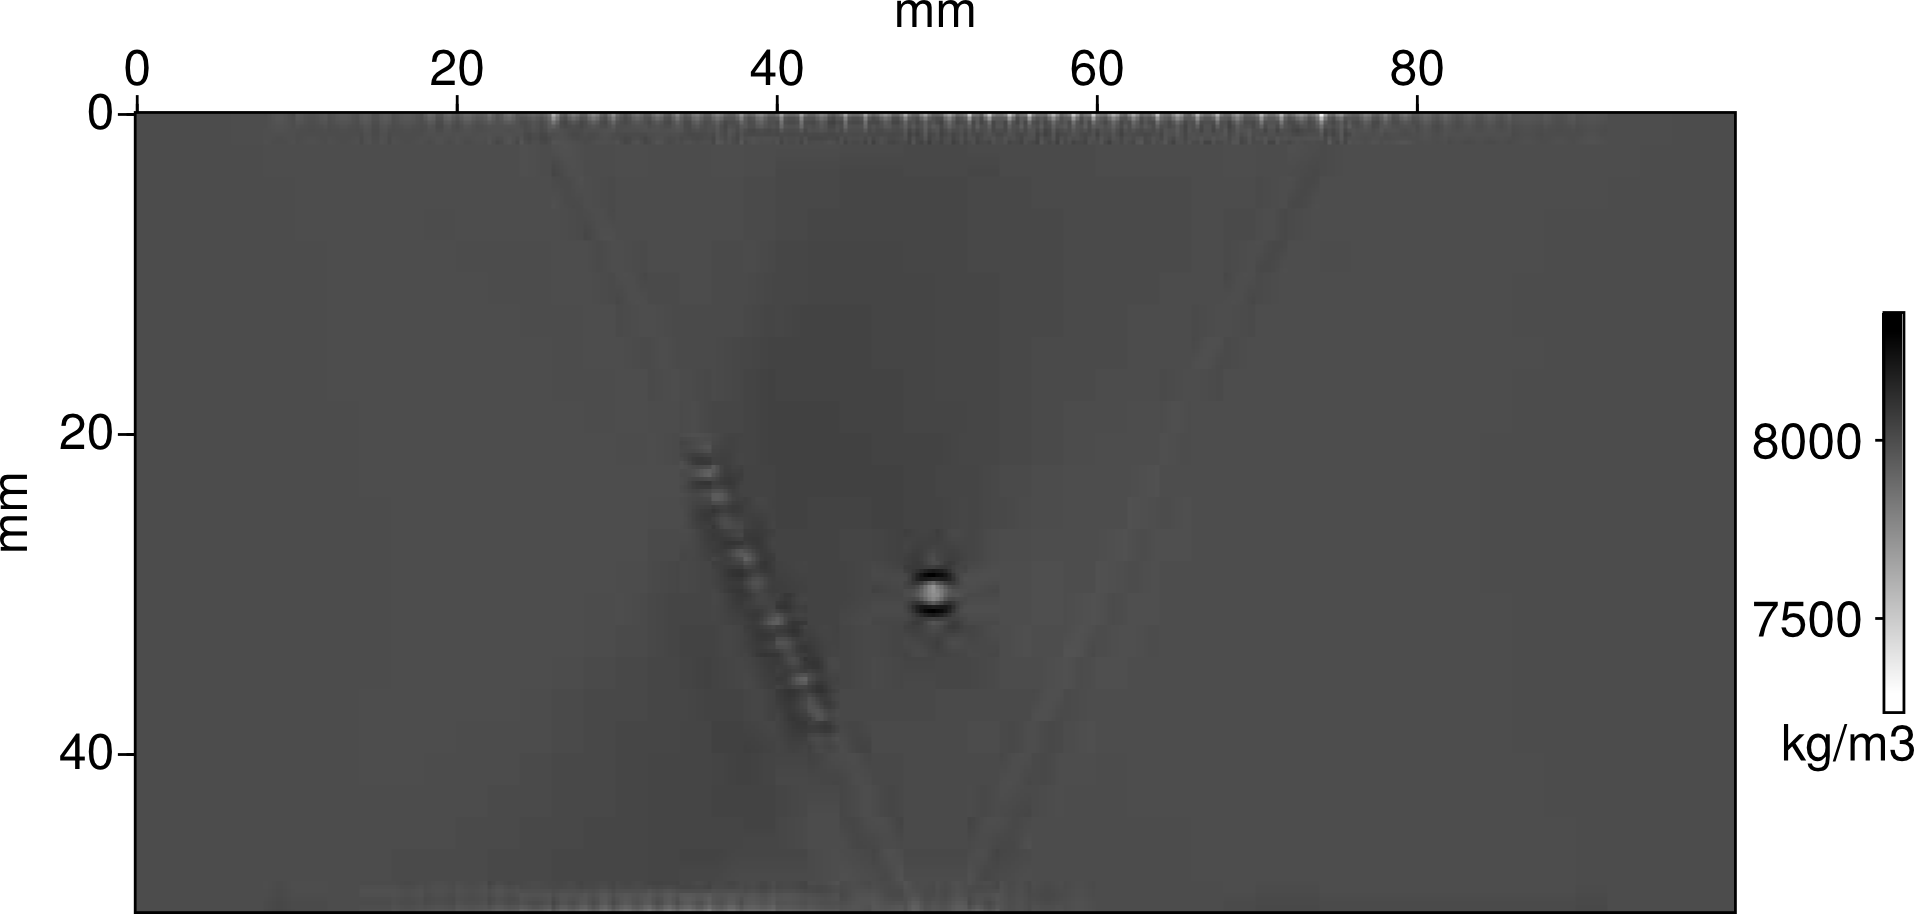
\includegraphics[height=1.9cm]{img/multi/rho_6000k.png}\\		
	\end{columns}

\end{frame}


%\subsection*{}
%\begin{frame}{\insertsectionhead}
%\begin{small}
%\begin{itemize}
%	\item Inversion monoparamètre : \\[0.2cm]
%	\begin{columns}
%		\column{0.5\textwidth}
%		\centering
%		Vitesse : \\[0.2cm]
%		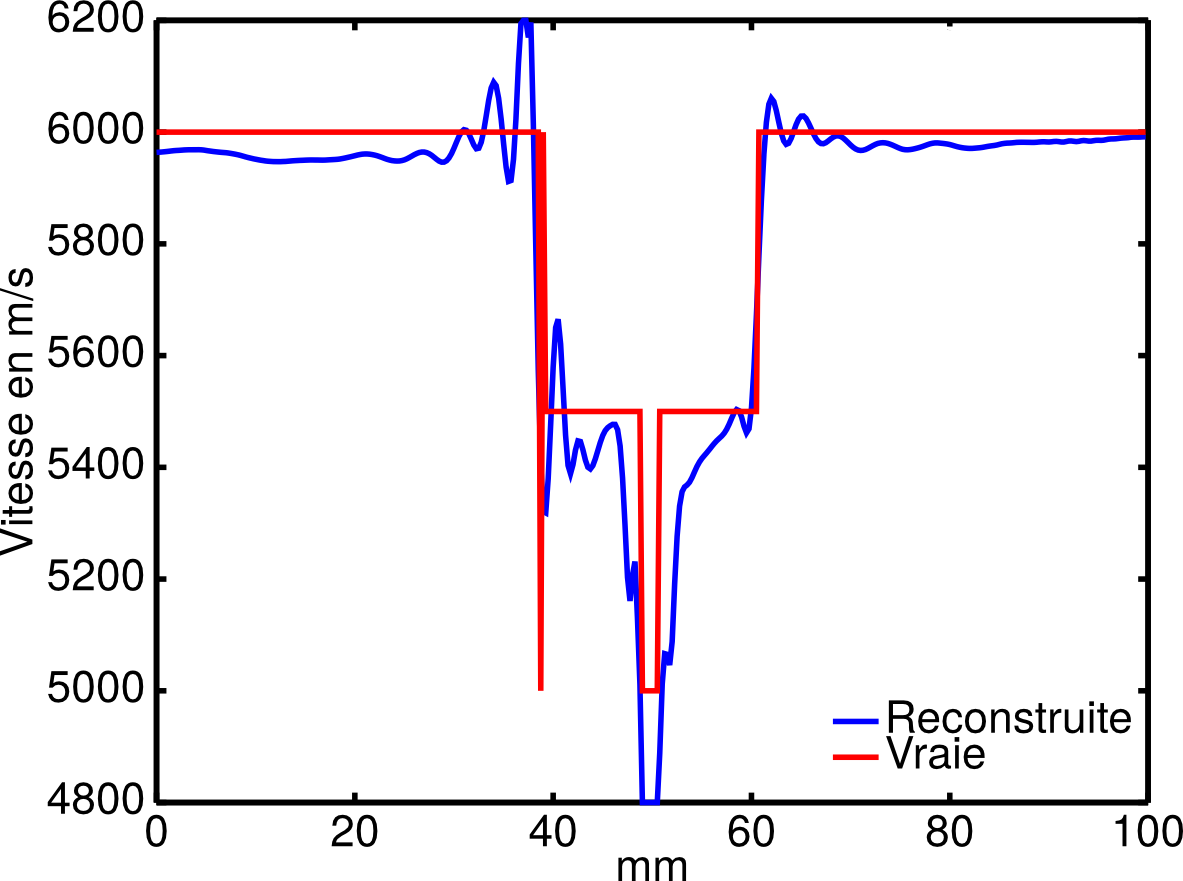
\includegraphics[width=0.6\textwidth]{img/multi/coupe_vp_mono_smooth_hor.png}\\
%		\column{0.5\textwidth}
%		\centering
%		Masse volumique  : \\[0.2cm]
%		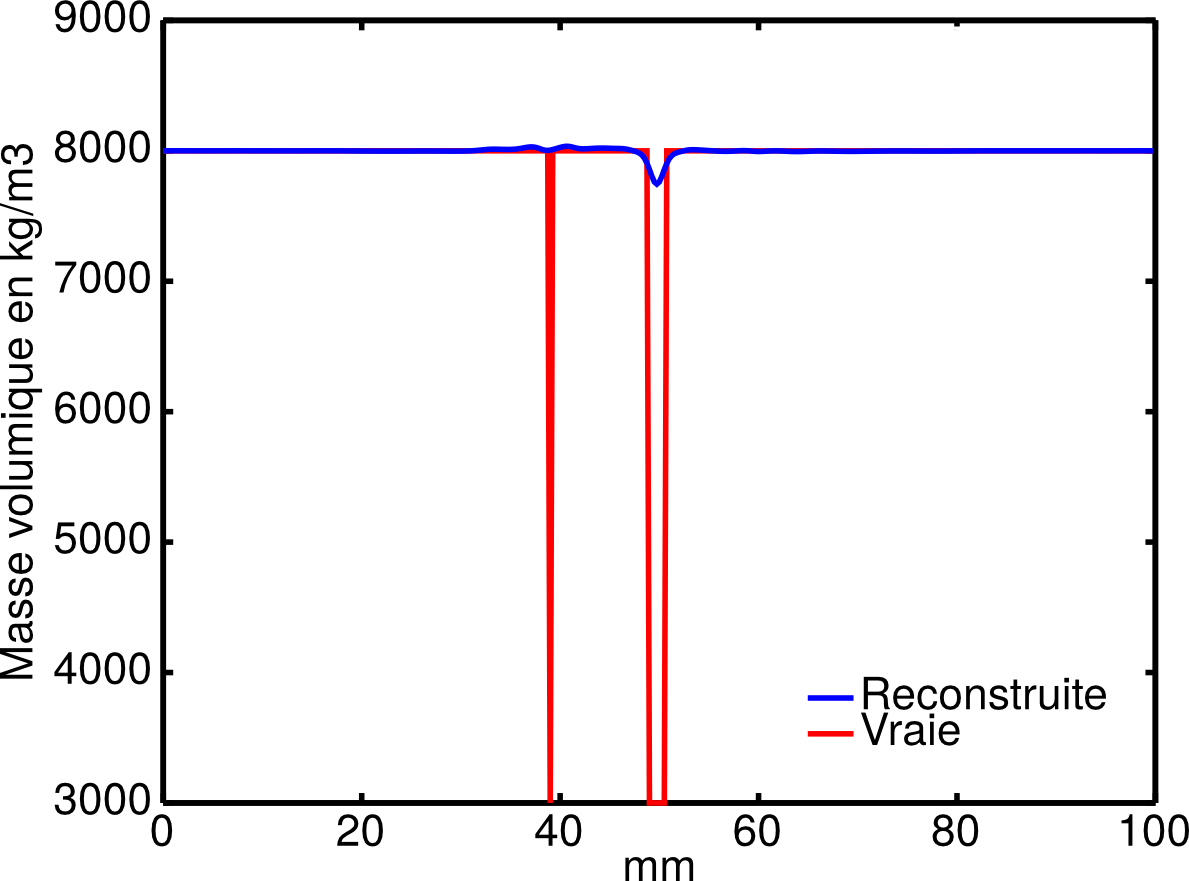
\includegraphics[width=0.6\textwidth]{img/multi/coupe_rho_mono.png}\\
%	\end{columns}
%	\item Inversion multiparamètre : \\[0.2cm]
%	\begin{columns}
%		\column{0.5\textwidth}
%		\centering
%		Vitesse : \\[0.2cm]
%		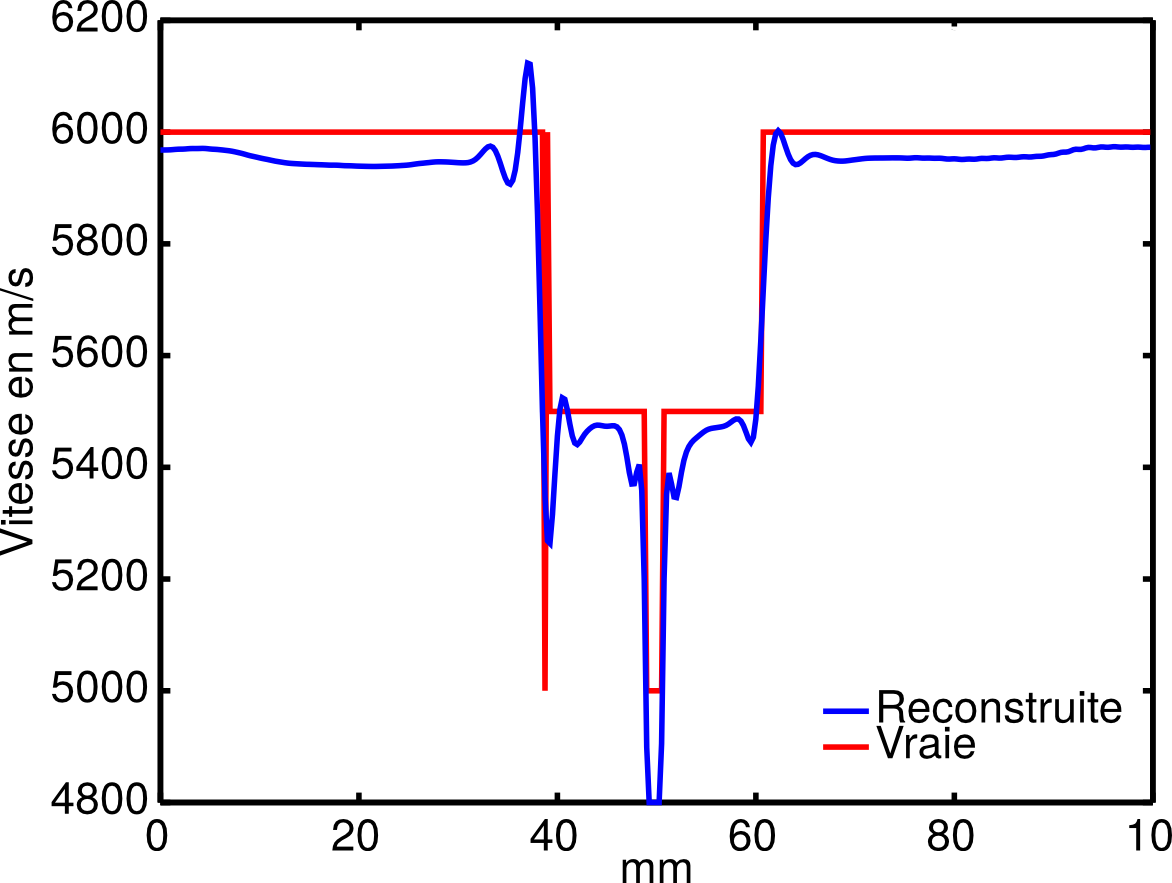
\includegraphics[width=0.6\textwidth]{img/multi/coupe_vp_multi.png}\\
%		\column{0.5\textwidth}
%		\centering
%		Masse volumique : \\[0.2cm]
%		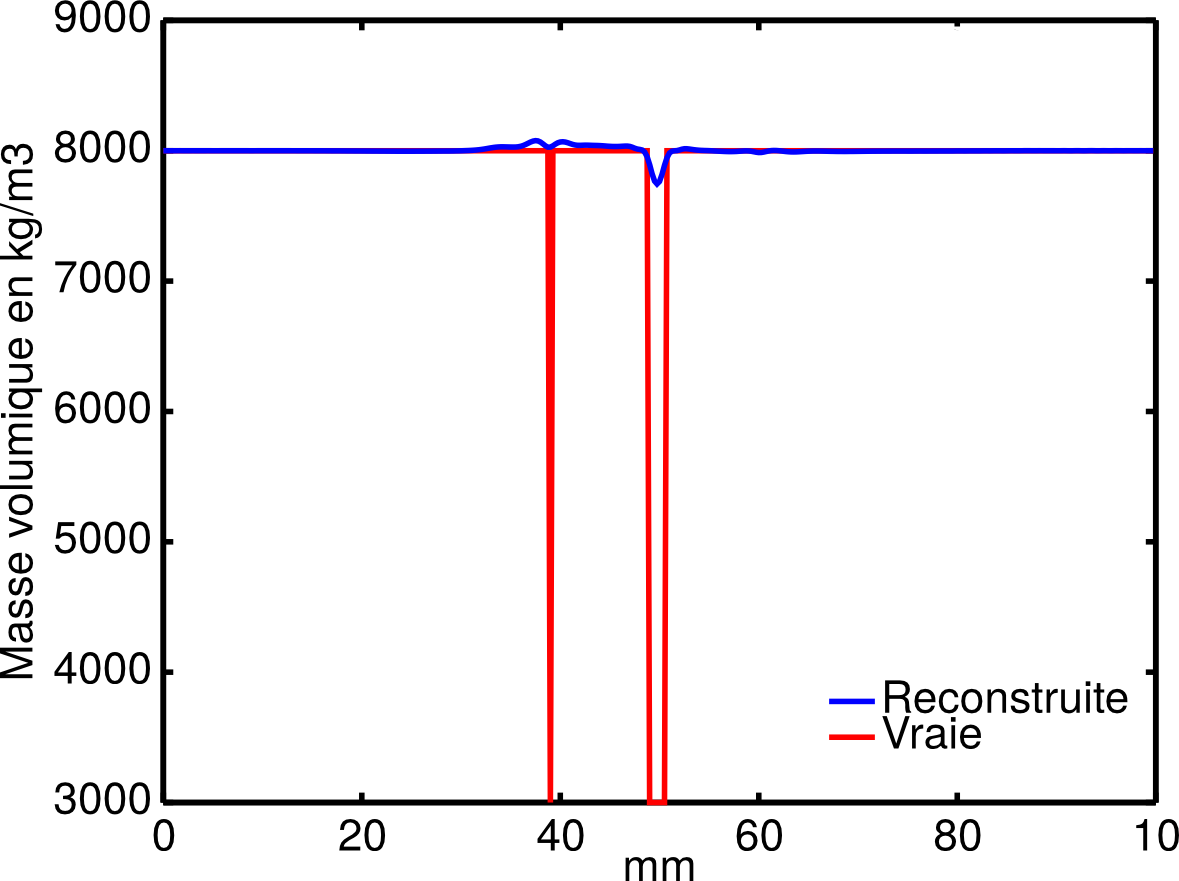
\includegraphics[width=0.6\textwidth]{img/multi/coupe_rho_multi.png}\\
%	\end{columns}
%	
%\end{itemize}
%\hspace{2.7cm}Coupes horizontales à 3 cm de profondeur
%\end{small}
%\end{frame}
%
%\begin{frame}{\insertsectionhead}
%\setlength{\leftmargin}{-2cm}
%\setlength{\rightmargin}{-2cm}
%%\setlength{\textwidth}{29cm}
%\begin{picture}(0,0)(0,0)\put(-20,-33){
%	$v_{p}$
%}\end{picture}
%\begin{picture}(0,0)(0,0)\put(-20,-87){
%	$\rho$
%}\end{picture}
%\vspace{-0.5cm}
%\begin{itemize}
%	\small{\item 9 inversions successives de 200 kHz à 3 MHz }
%\end{itemize}
%\vspace{0.3cm}
%	\begin{columns}
%		\column{0.3\textwidth}
%		\centering
%		\scriptsize{Modèles initiaux}
%		\includegraphics[height=1.9cm]{img/vp_mono_smooth/vp_smooth.png}\\
%		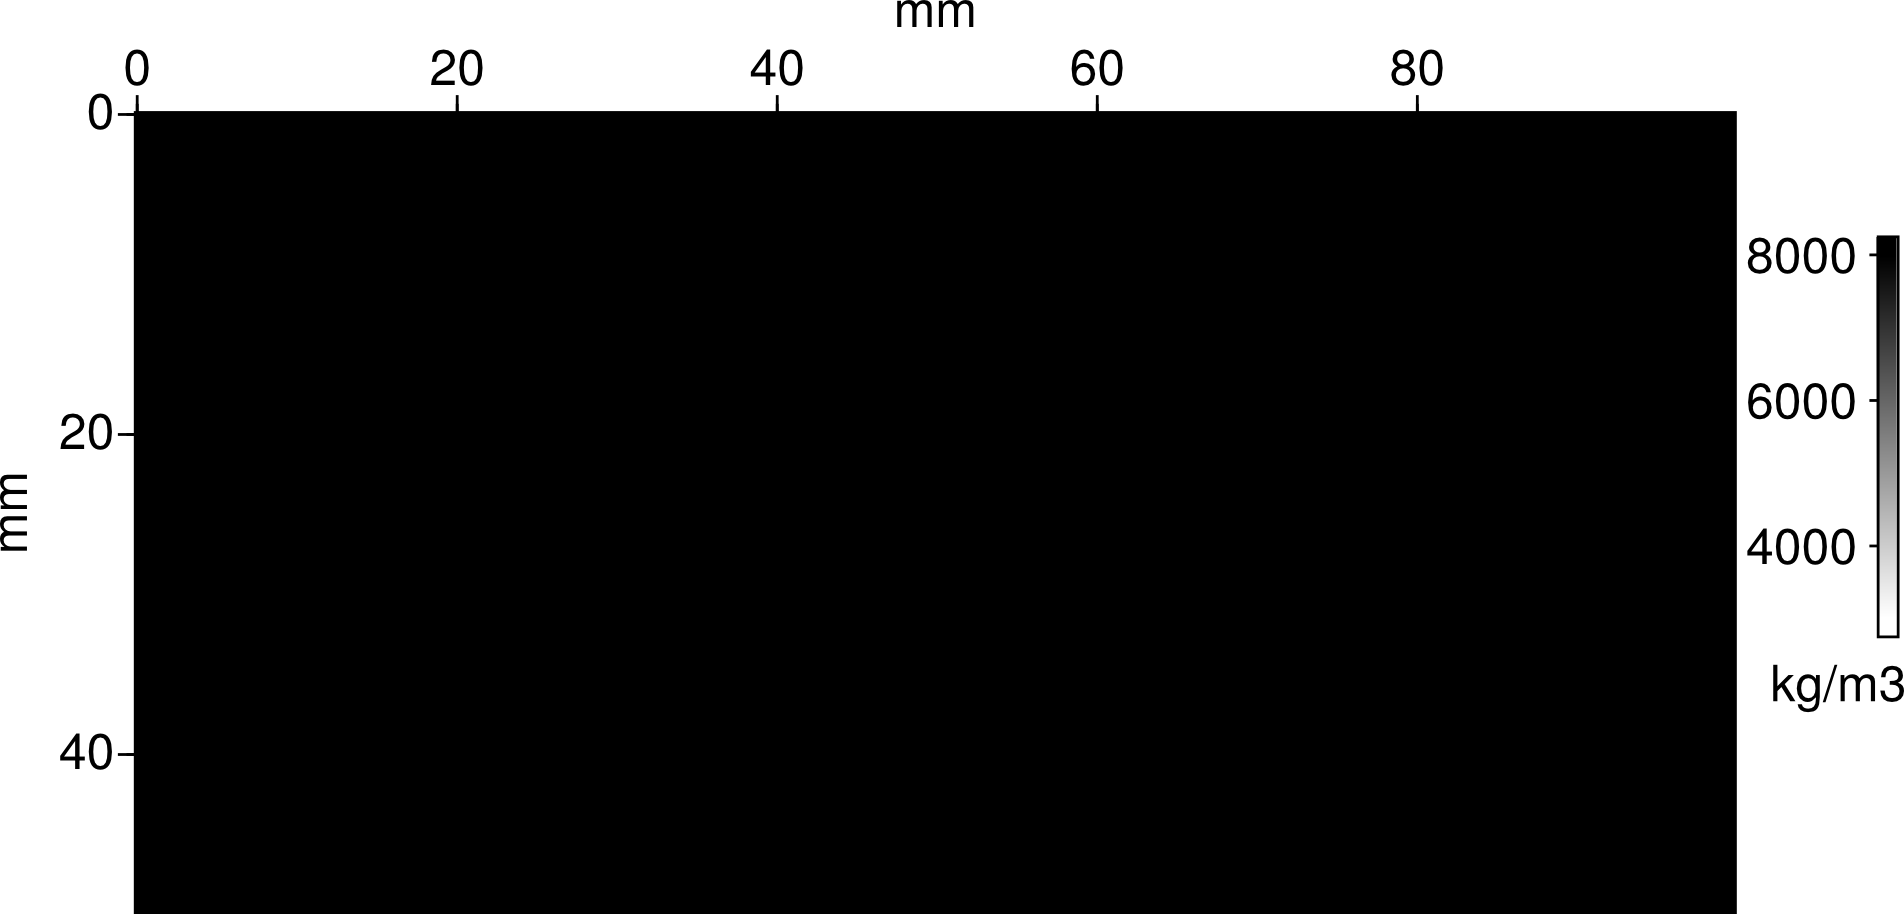
\includegraphics[height=1.9cm]{img/rho_mono/rho_init.png}		
%		\column{0.3\textwidth}
%		\centering
%		\scriptsize{Inversions monoparamètres}
%		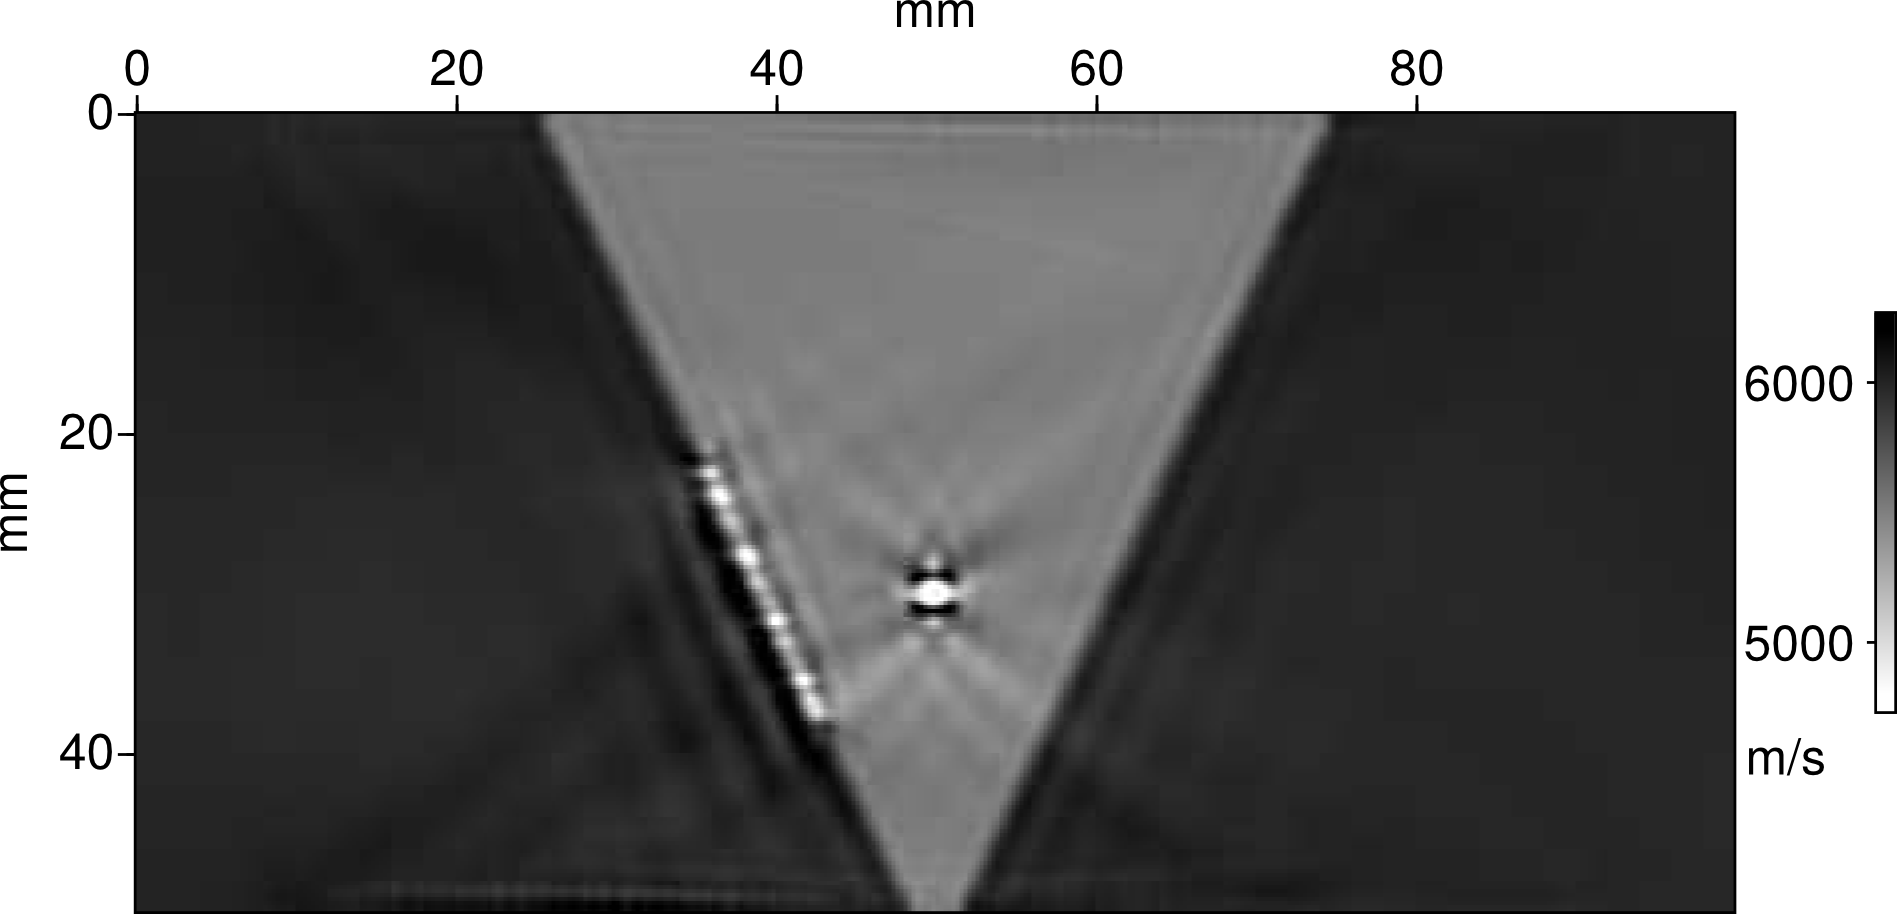
\includegraphics[height=1.9cm]{img/vp_mono_uni/vp_3300k.png}\\
%		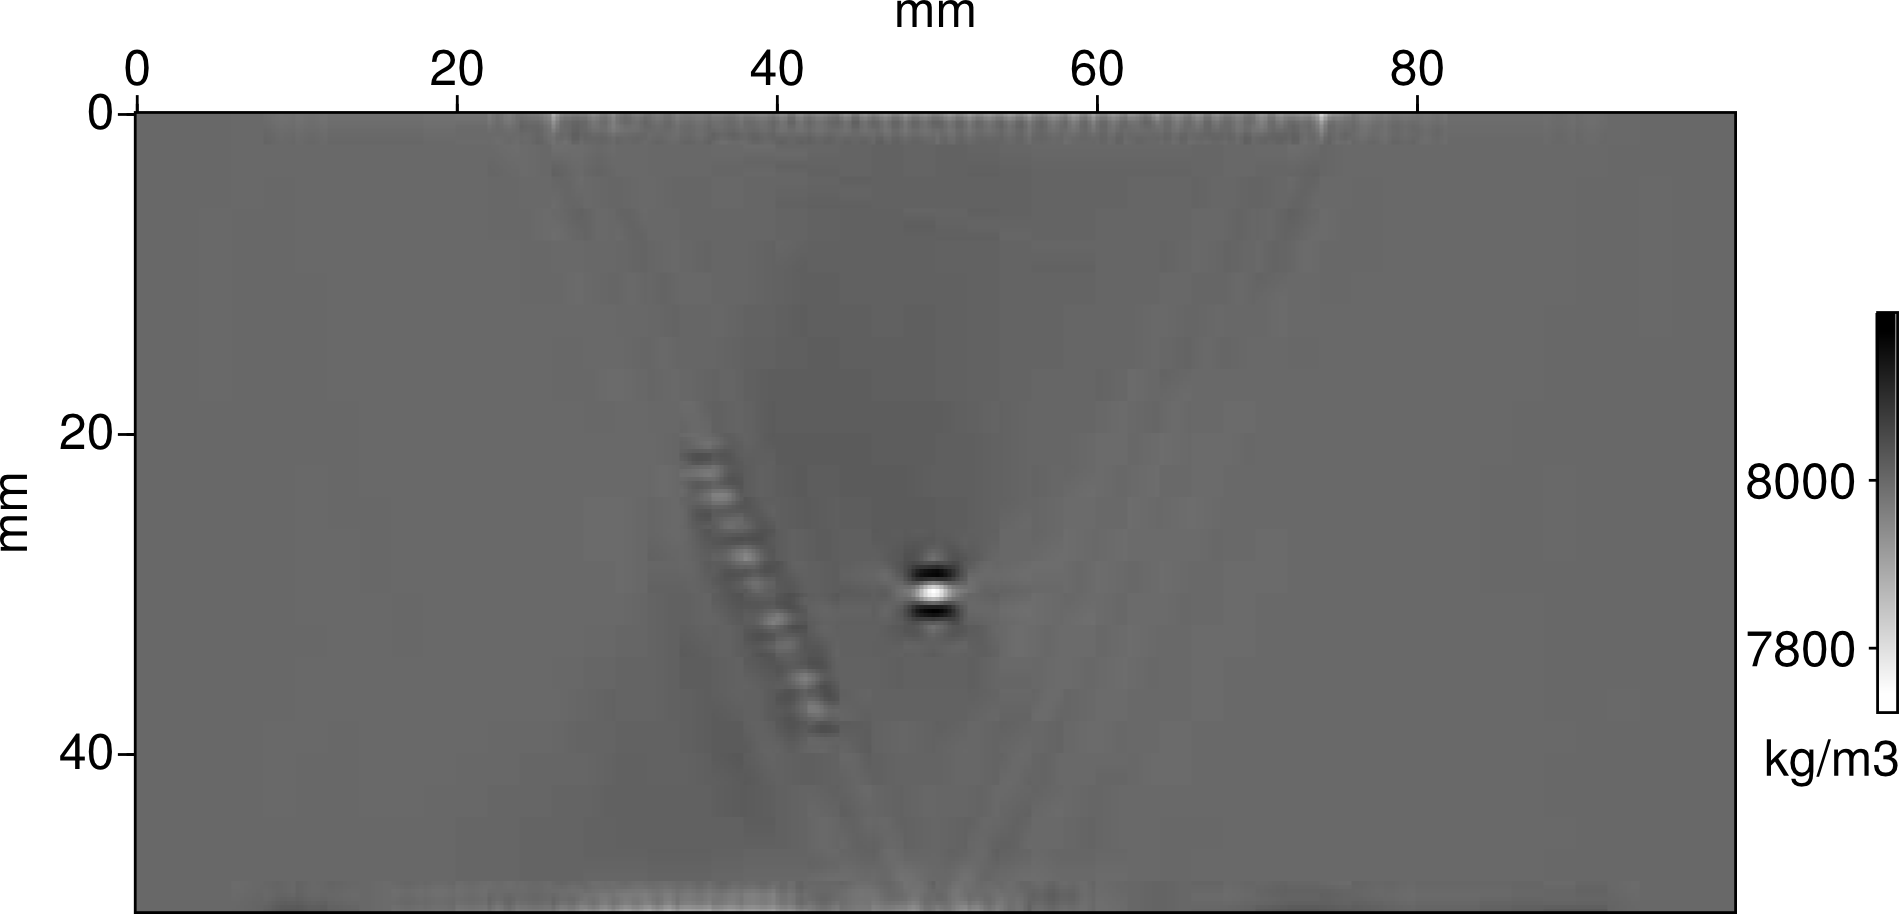
\includegraphics[height=1.9cm]{img/rho_mono/rho_mono.png}		
%		\column{0.3\textwidth}
%		\centering
%		\scriptsize{Inversion multiparamètre}
%		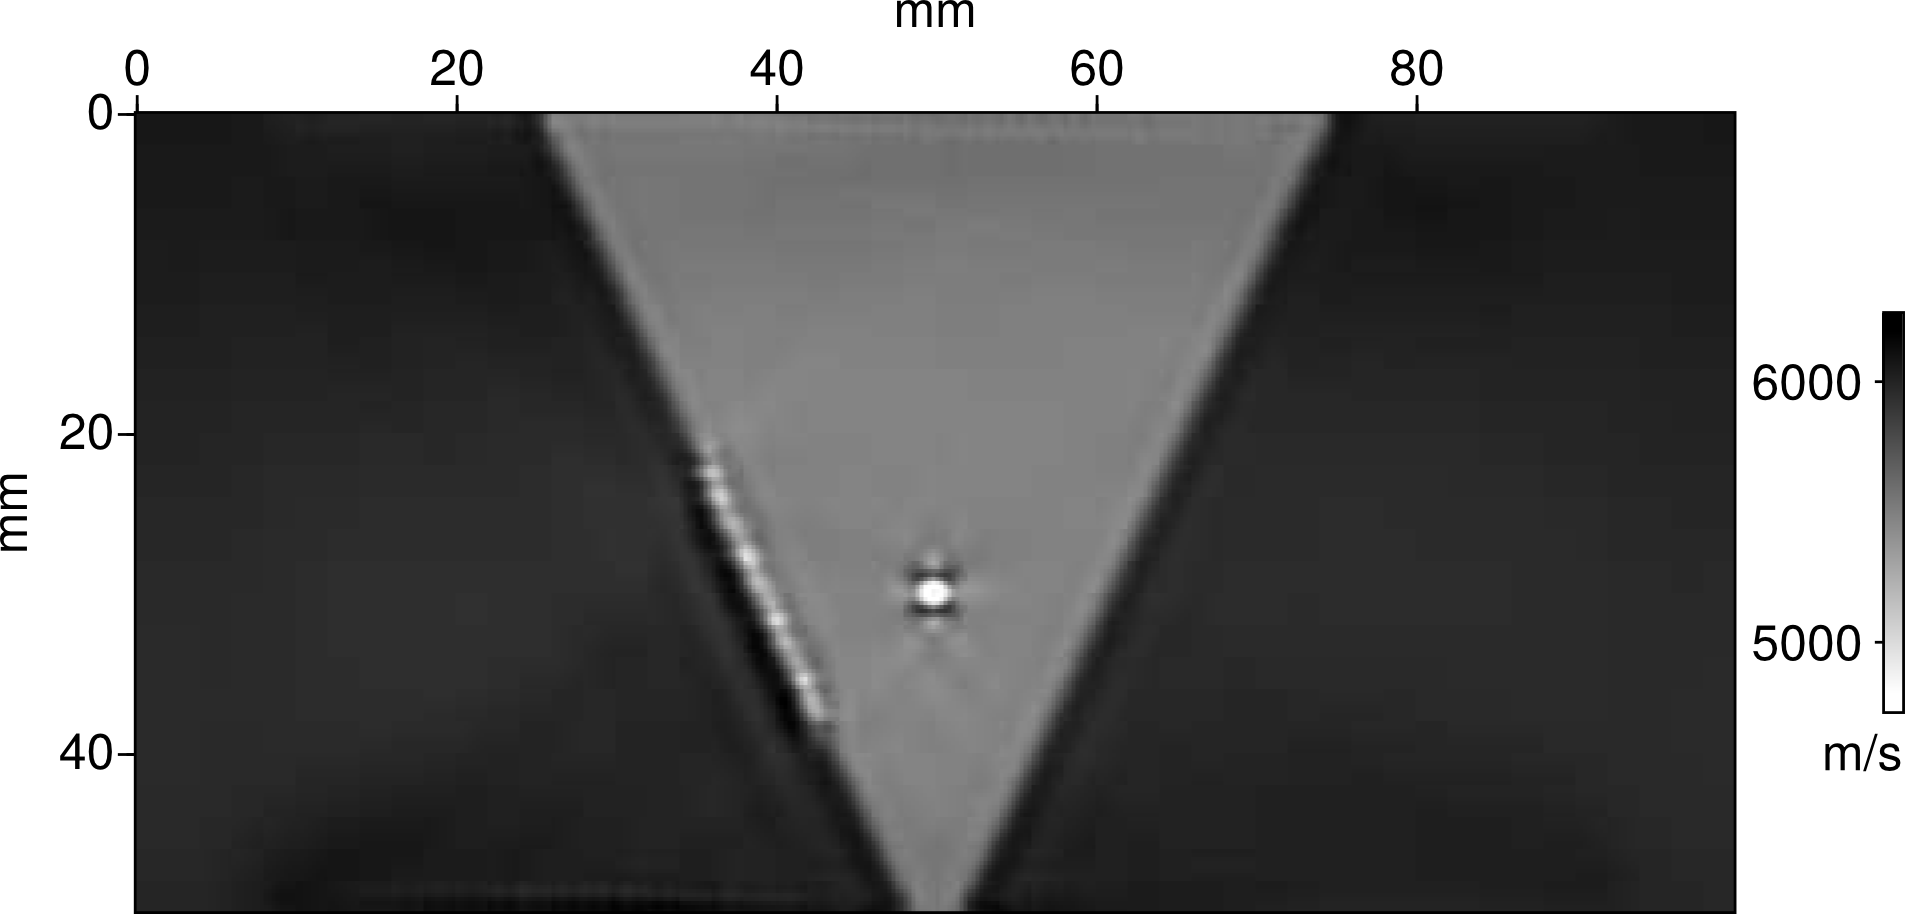
\includegraphics[height=1.9cm]{img/multi/vp_multi_6000k.png}\\		
%		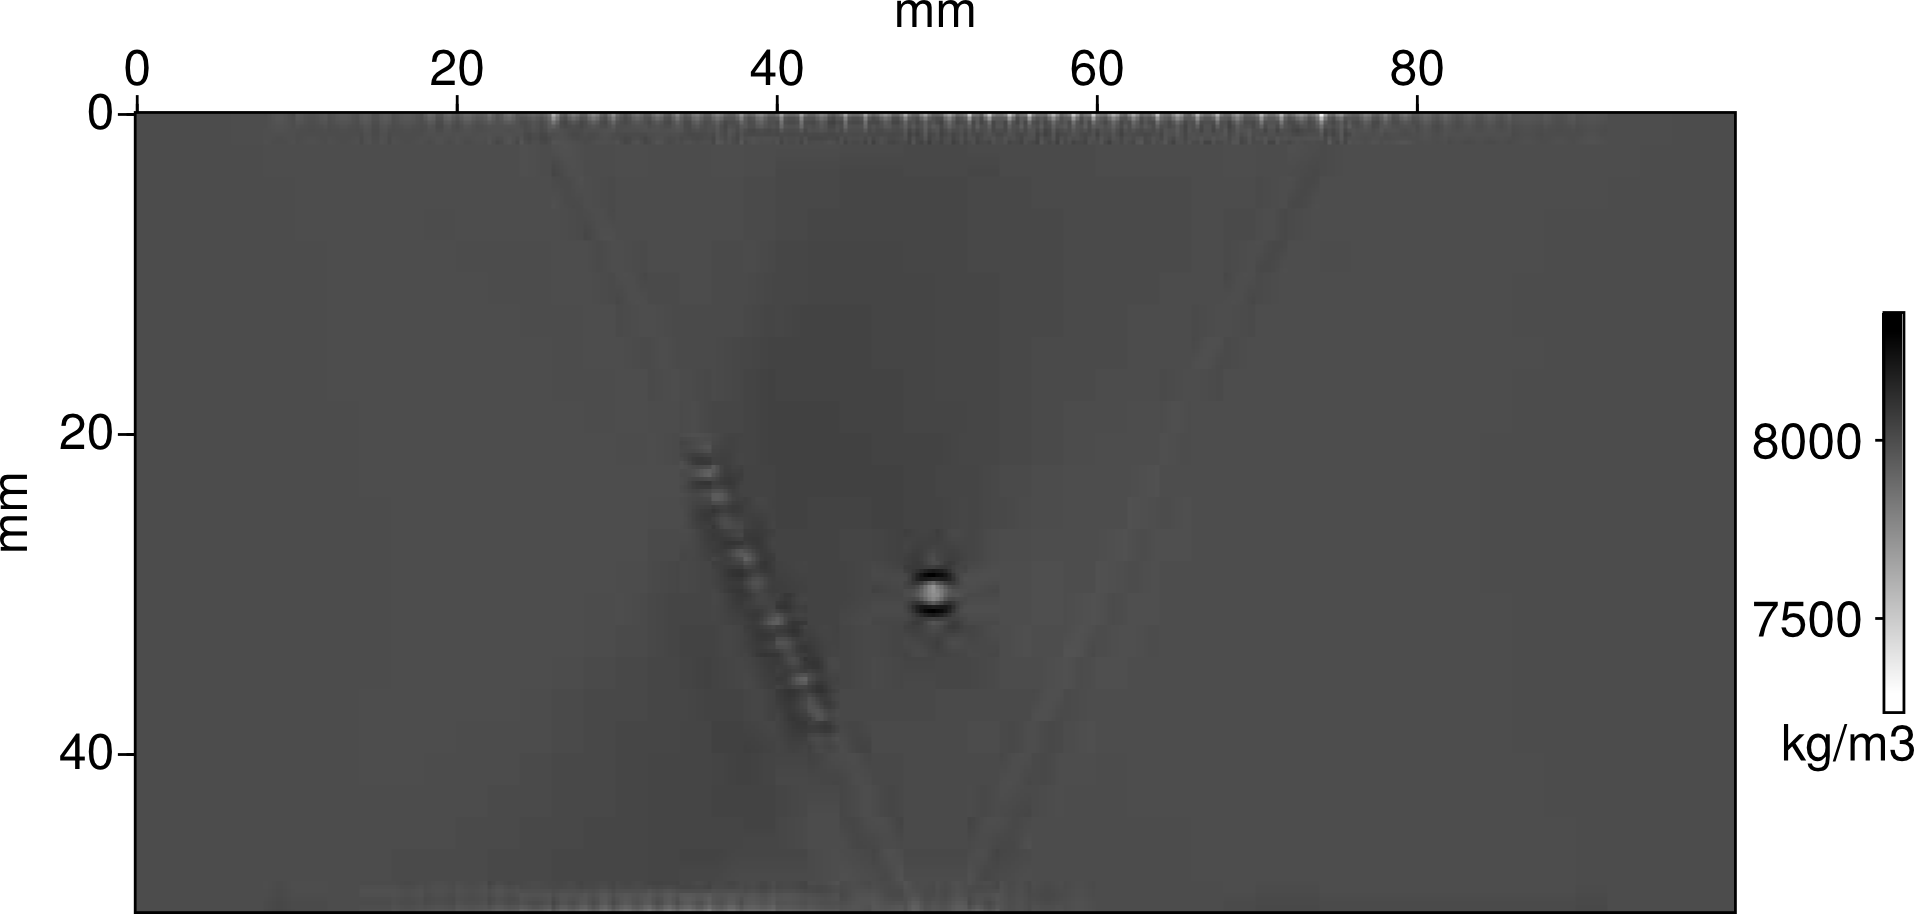
\includegraphics[height=1.9cm]{img/multi/rho_6000k.png}\\		
%	\end{columns}
%	\vspace{0.5cm}
%	\onslide<2->{
%		\begin{columns}
%			\column{0.6\textwidth}
%			\small{
%			\begin{itemize}
%				\item Comparaison avec le beamformign\\[0.3cm]
%			\end{itemize}
%			 \centering
%			\begin{equation*}
%				I(\bm{r})= \displaystyle\sum_{r} \displaystyle\sum_{e} s_{r,e}\left( T_{\bm{r}\bm{r}_{r}+T_{\bm{r}\bm{r}_{e}}} \right)
%			\end{equation*}
%			}
%			\column{0.4\textwidth}
%			\centering
%			\includegraphics[height=2.5cm]{img/tfm_retouche.png}
%		\end{columns}
%	}
%\end{frame}




\section{Conclusions, perspectives}

\begin{frame}{Conclusion}

%	\begin{wrapfigure}{r}{3.5cm}
%		\centering
%		\vspace{-1.2cm}\includegraphics[width=3.7cm]{img/data_3D/data_2freesurf.png}\\
%		\tiny{En bleu : réflexions OS sur PML (plan (xz))\\
%		En rouge : réflexion P et S de l'onde P sur l'inclusion\\
%		En vert : réflexion OS sur PML gauche  (plan (zy))}
%		\vspace{-5.3cm}
%	\end{wrapfigure}~
	\begin{itemize}
		\item<1-> Inversion multiparamètre : corrige les artefacts\\
		 \item<2-> Régularisation empirique hiérarchique : 
		\begin{itemize}
			\item Gamme fréquentielle
			\item Paramétrisation
			\item Sources et récepteurs
			\item Filtrage temporel
		\end{itemize}~\\
		\item<3-> Temps de calcul (2D) : \\
		9 fréq. x 20 perturbations = 180 inversions\\
		5 min/inversion $\rightarrow$ 15h\\
		VS beamforming : 10 min sur pc\\~\\~\\		
				
	\end{itemize}
\end{frame}

\begin{frame}{Perspectives}
\setlength{\leftmargin}{-1cm}
\setlength{\rightmargin}{-1cm}

	\begin{itemize}

		\item<1-> Prise en compte de l'anisotropie, 3D : $6 \times C_{ij}$
		\begin{figure}[!h]
		    \centering
		    \hspace{-1cm}\begin{subfigure}[b]{0.25\textwidth}
		    	\centering
		 		\includegraphics[height=2cm]{img/ogilvy_model.png}
		 		\vspace{0.2cm}\caption{\centering \scriptsize Modèle d'orientation des grains}
			\end{subfigure}
			\begin{subfigure}[b]{0.7\textwidth}
				\centering
		 		\includegraphics[height=2cm]{img/ogilvy_ray1.png}
		 		\includegraphics[height=2cm]{img/ogilvy_ray2.png}\\
		 		\raggedright{\vspace{-0.25cm}\tiny{\itshape Images extraites de~Ogilvy, 1986}}
		 		\caption{\scriptsize Courbure des rayons (ondes de compressions) \\~}
			\end{subfigure}\\
				
		\end{figure}	
		\item<2-> Élaboration d'un modèle initial fiable 
		\item<3-> Application à des données expérimentales
%		\item<5-> Prise en compte de la propagation 3D
%	\end{itemize}
%	\begin{picture}(0,0)(0,0)\put(240,0){
%		\only<5->{
%		\begin{tikzpicture}
%			\node (a) at (0,0) {\includegraphics[width=2.5cm]{img/linear_array.png}};
%			\node (b) [below=-0.2cm of a] {\tiny \itshape Image Olympus};
%		\end{tikzpicture}
%		}
%	}\end{picture}
	\end{itemize}
	
\end{frame}




\begin{frame}
	 	Codes ouverts (FORTRAN 90) : \url{ http://seiscope2.osug.fr}\\
		 $\hookrightarrow$optimization toolbox + codes pb direct/inverse\\~\\
		Transport optimal (norme de Kantorovich-Rubinstein), Métivier 2016\\
		Prior informations, Asnaashari 2013\\

\end{frame}

